% ======================================================================
%DIF LATEXDIFF DIFFERENCE FILE
%DIF DEL /home/qermez/Desktop/Coev_balance_PLOS_ONE/revision/resubmission/source_support/original_main_for_diff.tex   Tue Oct 27 09:27:32 2026
%DIF ADD /home/qermez/Desktop/Coev_balance_PLOS_ONE/revision/resubmission/source_support/revision_main_for_diff.tex   Thu Nov  5 12:39:56 2026
% PLOS ONE submission -- prepared from the official PLOS LaTeX template
% (Version 3.8, April 2026). Bibliography style: plos2025.bst
% ======================================================================
\documentclass[10pt,letterpaper]{article}
\usepackage[top=0.85in,left=2.75in,footskip=0.75in]{geometry}
\usepackage{tabularx}
\usepackage{seqsplit}
\usepackage{booktabs}
\usepackage{amsmath,amssymb}
\usepackage{changepage}
\usepackage{textcomp,marvosym}
\usepackage{cite}
\usepackage{nameref,hyperref}
%DIF 15a15
\hypersetup{hidelinks} %DIF > 
%DIF -------
\usepackage[right]{lineno}
\usepackage[nopatch=eqnum]{microtype}
\microtypesetup{expansion=false}
\DisableLigatures[f]{encoding = *, family = * }
\usepackage[table]{xcolor}
\usepackage{array}

% --- packages required by this manuscript's tables/figures ---
\usepackage[T1]{fontenc}
\usepackage{float}
\usepackage{multirow}
\usepackage{booktabs}

% create "+" rule type for thick vertical lines
\newcolumntype{+}{!{\vrule width 2pt}}
\newlength\savedwidth
\newcommand\thickcline[1]{%
  \noalign{\global\savedwidth\arrayrulewidth\global\arrayrulewidth 2pt}%
  \cline{#1}%
  \noalign{\vskip\arrayrulewidth}%
  \noalign{\global\arrayrulewidth\savedwidth}%
}
\newcommand\thickhline{\noalign{\global\savedwidth\arrayrulewidth\global\arrayrulewidth 2pt}%
\hline
\noalign{\global\arrayrulewidth\savedwidth}}

% Remove comment for double spacing
\usepackage{setspace}
\doublespacing

% Text layout
\raggedright
\setlength{\parindent}{0.5cm}
\textwidth 5.25in
\textheight 8.75in

% Bold 'Fig #' in caption, period separator, left justified
\usepackage[aboveskip=1pt,labelfont=bf,labelsep=period,justification=raggedright,singlelinecheck=off]{caption}
\renewcommand{\figurename}{Fig}

% Please use the included `plos2025.bst` as the BibTeX style
\bibliographystyle{../../plos2025}

% Remove brackets from numbering in List of References
\makeatletter
\renewcommand{\@biblabel}[1]{\quad#1.}
\makeatother

% Header and Footer with logo
\usepackage{lastpage,fancyhdr,graphicx}
\usepackage{epstopdf}
\pagestyle{fancy}
\fancyhf{}
\rfoot{\thepage/\pageref{LastPage}}
\renewcommand{\headrulewidth}{0pt}
\renewcommand{\footrule}{\hrule height 2pt \vspace{2mm}}
\fancyheadoffset[L]{2.25in}
\fancyfootoffset[L]{2.25in}
\lfoot{\today}
 %DIF > 
 %DIF > 
\def\SubmissionVersion{1} %DIF > 
\newif\ifillustrated %DIF > 
\ifdefined\SubmissionVersion\illustratedfalse\else\illustratedtrue\fi %DIF > 
\newcommand{\paperfigure}[4]{% %DIF > 
  \par\begin{center}\begin{minipage}{\linewidth}\centering %DIF > 
  \ifillustrated\includegraphics[width=\linewidth,height=.60\textheight,keepaspectratio]{figures/#1.pdf}\par\fi %DIF > 
  \captionof{figure}{\textbf{#2.} #3}\label{#4} %DIF > 
  \end{minipage}\end{center}\par %DIF > 
} %DIF > 
%DIF PREAMBLE EXTENSION ADDED BY LATEXDIFF
%DIF UNDERLINE PREAMBLE %DIF PREAMBLE
\RequirePackage[normalem]{ulem} %DIF PREAMBLE
\RequirePackage{color}\definecolor{RED}{rgb}{1,0,0}\definecolor{BLUE}{rgb}{0,0,1} %DIF PREAMBLE
\providecommand{\DIFaddtex}[1]{{\protect\color{blue}\uwave{#1}}} %DIF PREAMBLE
\providecommand{\DIFdeltex}[1]{{\protect\color{red}\sout{#1}}}                      %DIF PREAMBLE
%DIF SAFE PREAMBLE %DIF PREAMBLE
\providecommand{\DIFaddbegin}{} %DIF PREAMBLE
\providecommand{\DIFaddend}{} %DIF PREAMBLE
\providecommand{\DIFdelbegin}{} %DIF PREAMBLE
\providecommand{\DIFdelend}{} %DIF PREAMBLE
\providecommand{\DIFmodbegin}{} %DIF PREAMBLE
\providecommand{\DIFmodend}{} %DIF PREAMBLE
%DIF FLOATSAFE PREAMBLE %DIF PREAMBLE
\providecommand{\DIFaddFL}[1]{\DIFadd{#1}} %DIF PREAMBLE
\providecommand{\DIFdelFL}[1]{\DIFdel{#1}} %DIF PREAMBLE
\providecommand{\DIFaddbeginFL}{} %DIF PREAMBLE
\providecommand{\DIFaddendFL}{} %DIF PREAMBLE
\providecommand{\DIFdelbeginFL}{} %DIF PREAMBLE
\providecommand{\DIFdelendFL}{} %DIF PREAMBLE
%DIF HYPERREF PREAMBLE %DIF PREAMBLE
\providecommand{\DIFadd}[1]{\texorpdfstring{\DIFaddtex{#1}}{#1}} %DIF PREAMBLE
\providecommand{\DIFdel}[1]{\texorpdfstring{\DIFdeltex{#1}}{}} %DIF PREAMBLE
\newcommand{\DIFscaledelfig}{0.5}
%DIF HIGHLIGHTGRAPHICS PREAMBLE %DIF PREAMBLE
\RequirePackage{settobox} %DIF PREAMBLE
\RequirePackage{letltxmacro} %DIF PREAMBLE
\newsavebox{\DIFdelgraphicsbox} %DIF PREAMBLE
\newlength{\DIFdelgraphicswidth} %DIF PREAMBLE
\newlength{\DIFdelgraphicsheight} %DIF PREAMBLE
% store original definition of \includegraphics %DIF PREAMBLE
\LetLtxMacro{\DIFOincludegraphics}{\includegraphics} %DIF PREAMBLE
\newcommand{\DIFaddincludegraphics}[2][]{{\color{blue}\fbox{\DIFOincludegraphics[#1]{#2}}}} %DIF PREAMBLE
\newcommand{\DIFdelincludegraphics}[2][]{% %DIF PREAMBLE
\sbox{\DIFdelgraphicsbox}{\DIFOincludegraphics[#1]{#2}}% %DIF PREAMBLE
\settoboxwidth{\DIFdelgraphicswidth}{\DIFdelgraphicsbox} %DIF PREAMBLE
\settoboxtotalheight{\DIFdelgraphicsheight}{\DIFdelgraphicsbox} %DIF PREAMBLE
\scalebox{\DIFscaledelfig}{% %DIF PREAMBLE
\parbox[b]{\DIFdelgraphicswidth}{\usebox{\DIFdelgraphicsbox}\\[-\baselineskip] \rule{\DIFdelgraphicswidth}{0em}}\llap{\resizebox{\DIFdelgraphicswidth}{\DIFdelgraphicsheight}{% %DIF PREAMBLE
\setlength{\unitlength}{\DIFdelgraphicswidth}% %DIF PREAMBLE
\begin{picture}(1,1)% %DIF PREAMBLE
\thicklines\linethickness{2pt} %DIF PREAMBLE
{\color[rgb]{1,0,0}\put(0,0){\framebox(1,1){}}}% %DIF PREAMBLE
{\color[rgb]{1,0,0}\put(0,0){\line( 1,1){1}}}% %DIF PREAMBLE
{\color[rgb]{1,0,0}\put(0,1){\line(1,-1){1}}}% %DIF PREAMBLE
\end{picture}% %DIF PREAMBLE
}\hspace*{3pt}}} %DIF PREAMBLE
} %DIF PREAMBLE
\LetLtxMacro{\DIFOaddbegin}{\DIFaddbegin} %DIF PREAMBLE
\LetLtxMacro{\DIFOaddend}{\DIFaddend} %DIF PREAMBLE
\LetLtxMacro{\DIFOdelbegin}{\DIFdelbegin} %DIF PREAMBLE
\LetLtxMacro{\DIFOdelend}{\DIFdelend} %DIF PREAMBLE
\DeclareRobustCommand{\DIFaddbegin}{\DIFOaddbegin \let\includegraphics\DIFaddincludegraphics} %DIF PREAMBLE
\DeclareRobustCommand{\DIFaddend}{\DIFOaddend \let\includegraphics\DIFOincludegraphics} %DIF PREAMBLE
\DeclareRobustCommand{\DIFdelbegin}{\DIFOdelbegin \let\includegraphics\DIFdelincludegraphics} %DIF PREAMBLE
\DeclareRobustCommand{\DIFdelend}{\DIFOaddend \let\includegraphics\DIFOincludegraphics} %DIF PREAMBLE
\LetLtxMacro{\DIFOaddbeginFL}{\DIFaddbeginFL} %DIF PREAMBLE
\LetLtxMacro{\DIFOaddendFL}{\DIFaddendFL} %DIF PREAMBLE
\LetLtxMacro{\DIFOdelbeginFL}{\DIFdelbeginFL} %DIF PREAMBLE
\LetLtxMacro{\DIFOdelendFL}{\DIFdelendFL} %DIF PREAMBLE
\DeclareRobustCommand{\DIFaddbeginFL}{\DIFOaddbeginFL \let\includegraphics\DIFaddincludegraphics} %DIF PREAMBLE
\DeclareRobustCommand{\DIFaddendFL}{\DIFOaddendFL \let\includegraphics\DIFOincludegraphics} %DIF PREAMBLE
\DeclareRobustCommand{\DIFdelbeginFL}{\DIFOdelbeginFL \let\includegraphics\DIFdelincludegraphics} %DIF PREAMBLE
\DeclareRobustCommand{\DIFdelendFL}{\DIFOaddendFL \let\includegraphics\DIFOincludegraphics} %DIF PREAMBLE
%DIF COLORLISTINGS PREAMBLE %DIF PREAMBLE
\RequirePackage{listings} %DIF PREAMBLE
\RequirePackage{color} %DIF PREAMBLE
\lstdefinelanguage{DIFcode}{ %DIF PREAMBLE
%DIF DIFCODE_UNDERLINE %DIF PREAMBLE
  moredelim=[il][\color{red}\sout]{\%DIF\ <\ }, %DIF PREAMBLE
  moredelim=[il][\color{blue}\uwave]{\%DIF\ >\ } %DIF PREAMBLE
} %DIF PREAMBLE
\lstdefinestyle{DIFverbatimstyle}{ %DIF PREAMBLE
	language=DIFcode, %DIF PREAMBLE
	basicstyle=\ttfamily, %DIF PREAMBLE
	columns=fullflexible, %DIF PREAMBLE
	keepspaces=true %DIF PREAMBLE
} %DIF PREAMBLE
\lstnewenvironment{DIFverbatim}{\lstset{style=DIFverbatimstyle}}{} %DIF PREAMBLE
\lstnewenvironment{DIFverbatim*}{\lstset{style=DIFverbatimstyle,showspaces=true}}{} %DIF PREAMBLE
%DIF END PREAMBLE EXTENSION ADDED BY LATEXDIFF

\AtBeginDocument{%
\newlabel{eq:bipolarity}{{2}{34}{Signed motif proportions and bipolarity}{equation.0.2}{}}
\newlabel{eq:hamiltonian}{{1}{33}{Coevolutionary Balance Theory}{equation.0.1}{}}
\newlabel{fig:enter-label}{{2}{9}{Whole-brain coevolutionary metrics for autistic (ASD) and typically developing (TD) adults after ComBat harmonization. Each panel shows the distribution of a global measure derived from the signed functional network: (top row, from left to right) total coevolutionary energy, the proportion of imbalanced-same links, and the proportion of agreement links; (bottom row, from left to right) the proportion of disagreement links and the proportion of imbalanced-opposite links. Boxplots display the median (central line), interquartile range (box), and 1.5~$\times $~IQR whiskers, with individual participants overlaid as jittered points (magenta/pink for ASD, green for controls). Raw and FDR-corrected $p$-values are shown above each panel. The panels shown are the whole-brain metrics with the smallest group-comparison $p$-values (proportion of agreement and imbalanced-same links); both showed only weak, uncorrected trends in ASD (more agreement and fewer imbalanced-same links) that did not survive FDR correction ($p_{\mathrm {FDR}} > 0.05$). Consistent with Table~\ref {tab:assumptions_and_tests}, no whole-brain coevolutionary metric differed significantly between groups after harmonization}{figure.caption.10}{}}
\newlabel{fig:flowchart}{{1}{5}{Overview of the analytical workflow used in this study. Resting state fMRI datasets from the ABIDE I repository were first preprocessed using the CPAC pipeline, including standard steps such as motion correction, spatial normalization, and temporal filtering. The preprocessed volumes were then parcellated into 200 regions of interest using the CC200 atlas, yielding a regional time series for each participant. For every region, the fractional amplitude of low frequency fluctuations (fALFF) was computed, and these values were binarized to define nodal activity states distinguishing relatively high from relatively low intrinsic activity. Pairwise functional connectivity between regions was estimated from the regional BOLD time series and converted into a signed adjacency matrix that captures the sign of the interaction between each pair of regions. Nodal states and signed links were combined within the coevolutionary balance framework to compute coevolutionary energy at different scales. Global and local graph efficiency were computed from the absolute-value weighted FC matrix. To mitigate multi-site batch effects, ComBat harmonization was applied to the derived network features prior to statistical analysis. Null networks were generated by randomizing nodal states or link signs while preserving the underlying graph topology, and group comparisons between ASD and TD adults were carried out on the resulting measures. Energy-derived features were subsequently used as input to machine learning classifiers. All analyses were repeated using both GSR-based and no-GSR (CompCor) preprocessing pipelines}{figure.caption.3}{}}
\newlabel{fig:hamil_correlates}{{9}{21}{Top 20 network metrics most strongly correlated with whole-brain coevolutionary energy ($H$) within the ASD group (no-GSR pipeline). Red bars indicate positive correlations (EnergyBlock features, which are negatively signed relatives of AvgFalffW and share the same information); blue bars indicate negative correlations. Note that AvgWeight features (pure FC magnitude, no fALFF-weighting) are also present among the strongest correlates, confirming that the Hamiltonian captures information beyond average connectivity. The two blue bars at the lower end of the ranking correspond to global and local graph efficiency; the global Hamiltonian is most directly compared with global efficiency, and the local efficiency measure provides the corresponding local-scale comparison. Their negative correlation with $H$ within ASD (FDR $p = 0.006$) indicates that more coevolutionarily stable networks tend to be less efficiently integrated}{figure.caption.34}{}}
\newlabel{fig:ml_confusion_roc}{{5}{16}{Receiver operating characteristic (ROC) curves for ASD versus TD classification on the held-out test set, GSR pipeline, after ComBat harmonization. The diagonal grey line indicates chance. Curves lie near the diagonal (best cross-validated accuracy $\approx 0.59$), indicating near-chance discrimination from the harmonized coevolutionary and connectivity features}{figure.caption.25}{}}
\newlabel{fig:ml_selected_features}{{7}{18}{Random-forest feature-importance ranking for ASD--TD classification (GSR pipeline, harmonized features). Because the classifiers performed at or near chance (Table~\ref {tab:ml_summary_full}), this ranking is exploratory and does not establish diagnostic relevance of any feature}{figure.caption.28}{}}
\newlabel{fig:noGSR_inter}{{11}{23}{Inter-network average connectivity metrics with the smallest $p$-values in the no-GSR sensitivity analysis. None survived FDR correction (all $p_{\mathrm {FDR}} > 0.35$). Effects are generally weaker and fewer than in the GSR-based analysis}{figure.caption.38}{}}
\newlabel{fig:noGSR_intra}{{10}{22}{Intra-network metric showing the largest uncorrected group difference in the no-GSR analysis: Dorsal Attention network average connectivity ($p = 0.039$, $p_{\mathrm {FDR}} = 0.32$). This did not survive FDR correction}{figure.caption.36}{}}
\newlabel{fig:noGSR_ml}{{12}{24}{ROC curves for ASD versus TD classification in the no-GSR sensitivity analysis (CompCor preprocessing, harmonized features). Curves lie near the chance diagonal; the best held-out test accuracy was $0.59$ (Gaussian Naive Bayes), again indicating near-chance discrimination, as in the GSR pipeline (Fig~\ref {fig:ml_confusion_roc})}{figure.caption.42}{}}
\newlabel{tab:GSR_comparison}{{11}{25}{Comparison of key results across pipelines after correct site harmonization, and the effect of harmonization itself. All group comparisons are FDR-corrected within their feature family. ``Pre-harm.'' denotes the earlier analysis in which ComBat had failed silently and raw features were used}{table.caption.44}{}}
\newlabel{tab:assumptions_and_tests}{{2}{8}{Summary of statistical procedures and group comparison tests for whole-brain coevolutionary metrics. The upper panel lists the main analysis steps and their purpose. The lower panel reports group comparison statistics (Mann--Whitney $U$ tests and independent $t$-tests where appropriate, selected based on Shapiro--Wilk normality tests and Levene's homogeneity test applied independently to each feature), raw $p$-values, and FDR-corrected $p$-values for ASD versus TD after ComBat harmonization (GSR pipeline, $n = 78$ ASD, $86$ TD). No whole-brain feature survived FDR correction}{table.caption.9}{}}
\newlabel{tab:behaviour_corr_expanded}{{6}{14}{Strongest associations between network metrics and clinical scores under the harmonized GSR pipeline. The table reports the strongest associations (by uncorrected Pearson $p$-value) from the full analysis of 92 features $\times $ 5 clinical scores (460 tests), together with the whole-brain Hamiltonian for reference. None survived FDR correction at $q < 0.05$ (all $p_{\mathrm {FDR}} > 0.59$). The number of nominally significant associations ($\approx 21$) is close to the chance expectation}{table.caption.20}{}}
\newlabel{tab:internetwork_new}{{4}{11}{Inter-network differences in average connectivity (AvgWeight), fALFF-aligned connectivity (AvgFalffW), and coevolutionary energy (EnergyBlock) between canonical resting-state networks. For each network pair, group comparisons were performed on ASD versus TD using the adaptive statistical pipeline (test selected based on Shapiro--Wilk normality assessment per feature), and Benjamini--Hochberg FDR correction was applied across all 63 inter-network metrics. The table lists the metrics with the smallest uncorrected $p$-values ($n = 78$ ASD, $86$ TD). No inter-network metric survived FDR correction at $\alpha = 0.05$; the SomatoMotor--Frontoparietal effect ($p_{\mathrm {FDR}} = 0.069$) is the closest and is treated as exploratory}{table.caption.15}{}}
\newlabel{tab:ml_best_model_metrics}{{8}{16}{Detailed metrics for the Gaussian Naive Bayes classifier (the model originally highlighted) on the held-out test set ($n = 34$) after ComBat harmonization. Performance is near chance. Precision, recall, and F1-score refer to the ASD class as the positive class; ROC AUC was computed from the predicted ASD class probabilities}{table.caption.24}{}}
\newlabel{tab:ml_summary_full}{{7}{16}{Performance of supervised classifiers for ASD versus TD classification using the selected coevolutionary and connectivity features after ComBat harmonization (GSR pipeline). CV accuracy was obtained from stratified 5-fold cross-validation on the training set (80\% of participants); test metrics were computed on the held-out 20\% test set ($n = 34$), which was not used at any stage of feature selection or hyperparameter tuning. No model exceeded chance in cross-validation}{table.caption.23}{}}
\newlabel{tab:network_results}{{3}{10}{Largest intra-network trends within the seven canonical Yeo resting-state networks under the harmonized GSR pipeline ($n = 78$ ASD, $86$ TD). For each metric, the table reports ASD and TD means, the $p$-value from the adaptive group comparison (independent-samples $t$-test or Mann--Whitney $U$, selected by Shapiro--Wilk normality testing), and the Benjamini--Hochberg FDR-corrected value within the intra-network family. \emph {No intra-network metric reached even nominal significance} ($p < 0.05$) after harmonization; values are listed for completeness}{table.caption.12}{}}
\newlabel{tab:noGSR_ml}{{10}{24}{Classification performance in the no-GSR sensitivity analysis (CompCor preprocessing) after ComBat harmonization. All models performed at or near chance (cross-validated accuracy $0.46$--$0.57$; held-out test accuracy $\leq 0.59$), consistent with the absence of FDR-significant univariate group differences}{table.caption.41}{}}
\newlabel{tab:noGSR_whole}{{9}{19}{Whole-brain coevolutionary metrics in the no-GSR sensitivity analysis (CompCor-based preprocessing). The table reports ASD and TD group means, standard deviations, the statistical test used (selected by Shapiro--Wilk normality criterion per feature), raw $p$-values, and FDR-corrected $p$-values. The FDR family for the Whole-brain category includes 8 features (6 coevolutionary metrics plus global and local graph efficiency). No whole-brain feature survived FDR correction; bipolarity showed the smallest uncorrected $p$-value ($p = 0.026$, $p_{\mathrm {FDR}} = 0.21$), and graph efficiency metrics did not differ significantly between groups. Compare with Table~\ref {tab:assumptions_and_tests} for the GSR-based primary analysis}{table.caption.31}{}}
\newlabel{tab:null_model_validation}{{1}{6}{Null-model validation statistics for whole-brain coevolutionary energy. After unified outlier removal, 78 ASD and 86 TD participants remained. For each subject, empirical energy was compared to the mean energy from topology-preserving null networks in which node states and edge signs were randomly permuted. Shapiro--Wilk tests confirmed normality of the difference distributions, justifying the use of paired $t$-tests alongside Wilcoxon signed-rank tests}{table.caption.6}{}}
\newlabel{tab:pls_results}{{5}{14}{Partial Least Squares regression cross-validation results (harmonized GSR pipeline). For each clinical score, the table reports the number of ASD subjects with valid data and the mean cross-validated $R^2$ for the single-component model. All values are negative, indicating that the models do not predict behavioral scores above chance---consistent with the univariate result that no feature--clinical score association survives FDR correction at $q < 0.05$, and with the underdetermined nature of the problem (90 features, $n = 29$--59)}{table.caption.19}{}}
\newlabel{tab:supp_corr_full}{{S6}{47}{\textbf {Summary statistics for the comprehensive correlation analysis.} Overview of the feature--clinical score correlation analysis, including sample sizes, number of tests, and significance thresholds}{table.caption.93}{}}
\newlabel{tab:supp_corr_sig}{{S5}{46}{\textbf {Full list of nominally significant feature--clinical score correlations (uncorrected $p < 0.05$).} The comprehensive analysis tested 460 correlations (92 features $\times $ 8 clinical scores). This table lists all 64 pairs that reached uncorrected significance for either Pearson or Spearman tests. None survived FDR correction. Sample sizes vary due to missing clinical data. The sign of $r$ is provided explicitly to allow unambiguous directional interpretation. A negative $r$ for Whole\_Energy\_global means more negative $H$ (more stable) is associated with higher ADOS (more severe); see main text for full directional interpretation}{table.caption.92}{}}
\newlabel{tab:supp_normality}{{S1}{39}{\textbf {Normality test summary per feature category.} For each of the 92 features tested (90 coevolutionary/connectivity features plus global and local graph efficiency), Shapiro--Wilk normality tests were conducted for the ASD and TD distributions independently. The decision rule was applied per feature: if both groups passed ($p > 0.05$), a standard $t$-test was used (or Welch's if Levene indicated unequal variances); if either group failed, Mann--Whitney $U$ was applied. The table summarizes the normality outcome by feature category. The predominance of non-parametric testing (87\% of features) reflects the empirical data distributions, not a post-hoc methodological choice}{table.caption.75}{}}
}
\begin{document}
\vspace*{0.2in}

% Title must be 250 characters or less.
\begin{flushleft}
{\Large
\textbf{Coevolutionary balance of resting-state brain networks in autism}
}
\newline
\\
S. Rezaei Afshar\textsuperscript{1},
G. R. Jafari\textsuperscript{2,*}
\\
\bigskip
\textbf{1} Institute for Cognitive and Brain Sciences, Shahid Beheshti University, Evin, Tehran, Iran
\\
\textbf{2} Department of Physics, Shahid Beheshti University, Evin, Tehran, Iran
\\
\bigskip

* Corresponding author: gjafari@gmail.com

\DIFaddbegin \medskip
\textbf{\DIFadd{Short title:}} \DIFadd{Coevolutionary balance in adult male autism
}

\DIFaddend \end{flushleft}

%DIF <  Please keep the abstract below 300 words
\DIFaddbegin \clearpage
\newgeometry{top=0.85in,left=1in,right=1in,footskip=0.75in}
\DIFaddend \section*{Abstract}
\DIFdelbegin \DIFdel{Autism spectrum disorder (ASD) involves atypical brain organization, yet the large-scale functional principles underlying these alterations remain incompletely understood. Here we examine whether
coevolutionary balance---a network-level energy measure derived from signed interactions and nodal
activity states---captures disruptions in resting-state functional connectivity in autistic adults. Using ABIDE I}\DIFdelend \DIFaddbegin \DIFadd{Signed functional connectivity and regional low-frequency BOLD fluctuations offer
complementary descriptions of }\DIFaddend resting-state \DIFdelbegin \DIFdel{fMRI data, we constructed whole-brain networks by combining binarized
fALFF activity with signed functional correlations and quantified their coevolutionary energy,
applying ComBat harmonization (after excluding single-participant sites) to mitigate multi-site
batch effects. Analyses were run under two preprocessing pipelines: }\DIFdelend \DIFaddbegin \DIFadd{organization. We examined their joint
alignment using a static Hamiltonian inspired by coevolutionary balance in a
male-only adult sample from ABIDE I. Downloaded preprocessed regional time series
and fALFF maps were analyzed with and without }\DIFaddend global signal regression (GSR\DIFdelbegin \DIFdel{,
primary) and CompCor-based denoising without GSR (sensitivity).
After harmonization and Benjamini--Hochberg correction, no whole-brain, intra-network, or inter-network feature differed
significantly between groups in either pipeline. The strongest nominal (uncorrected)whole-brain
trends were pipeline-dependent: with GSR, the ASD group showed marginally more negative global
coevolutionary energy ($-139.7$ vs. \ $-118.8$; uncorrected $p = 0.048$, $p_{\mathrm{FDR}} = 0.19$),
whereas without GSR, ASD showed marginally higher bipolarity (uncorrected $p = 0.026$,
$p_{\mathrm{FDR}} = 0.21$);
neither survived correction. Behavioral correlations, partial
least squares regression, }\DIFdelend \DIFaddbegin \DIFadd{).
Age and IQ eligibility yielded 140 participants (69 autistic participants and
71 controls). Measurement coverage defined a fixed common set of 106 regions;
site-adjusted group models included 136 participants. In a separate male-control
baseline, mean empirical Hamiltonian values were lower than their null expectations
under unrestricted and network/hemisphere-blocked state permutations. Hamiltonian values did not
show a detectable diagnosis effect after adjustment for site, age, full-scale IQ,
}\DIFaddend and \DIFdelbegin \DIFdel{partial least squares correlation analyses revealed no significant or
cross-validated brain--behavior structure. Within the ASD group, however,
global coevolutionary
energy was robustly associated with graph efficiency and with mean connectivity (e.g., }\DIFdelend \DIFaddbegin \DIFadd{mean framewise displacement (GSR: coefficient 1.43, 95\% CI $-17.17$ to 20.04;
}\DIFaddend no-GSR\DIFdelbegin \DIFdel{global
efficiency: $r = -0.33$, $p_{\mathrm{FDR}} = 0.005$), indicating that the framework behaves
coherently as a description of signed network organization even where group contrasts are absent.
We emphasize a methodological finding of independent value: an apparently significant whole-brain
energy difference that was present before site harmonization did not survive correct harmonization, illustrating how strongly multi-site variance can masquerade as an ASD--control effect in
signed-network analyses of ABIDE. Coevolutionary balance is therefore a coherent and interpretable
framework for signed brain networks, but in this adult ABIDE sample it did not reveal site-robust
group differences; we report this as a rigorous, transparent result. }\DIFdelend \DIFaddbegin \DIFadd{: 2.06, 95\% CI $-12.39$ to 16.50; both Holm-adjusted $p=1.00$).
ComBat, pooled energy-trimming, and larger-node-set sensitivities did not identify
a corrected diagnosis effect. Equivalence tests were inconclusive. Exploratory
site-held-out classification yielded balanced accuracies of 0.457--0.558, with
all conditional confidence intervals including 0.5.
A broader exploratory selection-method search did not establish a reliable performance gain. Clinical analyses and
motion- and mean-connectivity-adjusted efficiency analyses provided no corrected
evidence of an association. These results do not establish group equivalence,
diagnostic utility, or an autism-specific energy--efficiency relationship.
Interpretation is restricted to the selected adult males, the coverage-limited
network, and the documented limits of the downloaded derivatives.
}\DIFaddend 

\clearpage
\newgeometry{top=0.85in,left=1in,right=1in,footskip=0.75in}
\linenumbers

\section*{Introduction}\DIFdelbegin %DIFDELCMD < 

%DIFDELCMD < %%%
\DIFdel{Autism spectrum disorder (ASD) is a heterogeneous neurodevelopmental condition marked by persistent
differences in social communication and the presence of restricted or repetitive patterns of behavior, interests, or activities }%DIFDELCMD < \cite{APA:2022ds}%%%
\DIFdel{.
The clinical presentation spans a broad range
of intellectual and
language abilities, from individuals with minimal spoken language and co-occurring intellectual disability to those with average or above average cognitive skills. Many
autistic individuals also show additional conditions such as attention difficulties, anxiety, sleep
problems,
and epilepsy, which can complicate both diagnosis and management.
Recent epidemiological
data indicate that the prevalence of ASD has continued to rise, with an estimated 2.76 percent of
eight year old children in the United States meeting diagnostic criteria in 2020 }%DIFDELCMD < \cite{Maenner:2023pr}%%%
\DIFdel{.
This combination of clinical heterogeneity, high prevalence, and complex etiological mechanisms
underscores the need for quantitative, biologically interpretable measures that capture how brain
organization differs in ASD.
}%DIFDELCMD < 

%DIFDELCMD < %%%
\DIFdel{Resting state functional MRI (rs-fMRI) has become a central tool for probing large scale functional
organizationin vivo.
By measuring spontaneous blood oxygenation level dependent (BOLD) fluctuations
in the absence of explicit task demands, rs-fMRI provides access to intrinsic activity patterns that
are thought to reflect ongoing coordination within and between distributed neural systems. Amplitude
based measures such as the amplitude of low frequency fluctuations
(ALFF) and the fractional ALFF
(fALFF) summarize the strength of BOLD oscillations in the 0.01 to 0.08 Hz range, with fALFF
quantifying the proportion of power within this band relative to the full detectable spectrum }%DIFDELCMD < \cite{Zang:2007al,Zou:2008fa}%%%
\DIFdel{. Functional connectivity (FC), typically estimated as the correlation
between regional BOLD time series, captures statistical coupling between brain regions }%DIFDELCMD < \cite{Smith:2013fc}%%%
\DIFdel{. Together, these measures allow one to view the brain as a network in which nodes are regional activity
profiles and edges represent the strength and sign of their temporal relationships}\DIFdelend \DIFaddbegin \linelabel{lin:introduction}
\DIFadd{Resting-state functional MRI provides several descriptions of brain organization}\DIFaddend .
\DIFdelbegin %DIFDELCMD < 

%DIFDELCMD < %%%
\DIFdel{A large body of graph-theoretic work has used such rs-fMRI networks to study ASD. Across multiple
cohorts and analytic choices, studies have reported alterations in both network segregation and
network integration in autistic individuals }%DIFDELCMD < \cite{assaf2010abnormal,10.3389/fnhum.2013.00458,Uddin2013,Smith:2013fc}%%%
\DIFdel{. Reported findings include reduced or atypical clustering, changes in modular structure,
altered
small-world properties, and differences in
path length and global efficiency within and across
large-scale systems such as the default mode network, salience network, and attention networks
}%DIFDELCMD < \cite{assaf2010abnormal,10.3389/fnhum.2013.00458}%%%
\DIFdel{.
Despite important methodological differences
between studies , these results converge on the idea that ASD involves altered large-scale functional
organization rather than focal abnormalities confined to isolated regions. However, in most of these
approaches, nodal activity measures (for example, fALFF) and edge weights (for example, }\DIFdelend \DIFaddbegin \DIFadd{Functional connectivity (FC) measures statistical dependence between regional
BOLD time series, whereas fractional amplitude of low-frequency fluctuations
(fALFF) describes the relative contribution of low-frequency fluctuations to the
sampled spectrum }\cite{Zou:2008fa}\DIFadd{. Neither quantity directly measures neuronal
firing rate. Regional fALFF differences have been reported in adult autism
}\cite{Itahashi2015revision}\DIFadd{, but such regional effects need not produce a difference
in a scalar summary combining fALFF ranks and }\DIFaddend FC\DIFdelbegin \DIFdel{strength
and
sign) are treated as separate ingredients, and descriptive summaries are computed on either the
connectivity structure or the activity pattern alone.
This separation makes it difficult to capture
emergent properties that depend on how activity and connectivity jointly align.
}\DIFdelend \DIFaddbegin \DIFadd{.
}\DIFaddend 

\DIFdelbegin \DIFdel{Several lines of neurobiological evidence point to the importance of such joint alignment. Intrinsic
activity and connectivity patterns are thought to be shaped by underlying }\DIFdelend \DIFaddbegin \DIFadd{Signed networks retain positive and negative associations, whose treatment can
materially affect network summaries }\cite{RubinovSporns2011}\DIFadd{. Structural balance
theory describes consistency among signed relationships }\cite{Heider:1946ac,cartwright1956}\DIFadd{.
Coevolutionary models introduce nodal states as well as signed interactions
}\cite{Kargaran:2021he,GhanbarzadehNoudehi2022}\DIFadd{. Here, these ideas motivate a static
alignment statistic. We do not estimate a dynamical coevolutionary process,
metabolic energy, or }\DIFaddend excitation--inhibition \DIFdelbegin \DIFdel{balance, synaptic homeostasis, and plasticity mechanisms }%DIFDELCMD < \cite{Yizhar2011,Dinstein2011}%%%
\DIFdel{.
Perturbations in these processes can alter both the amplitude of spontaneous activity and the pattern
of long-range coupling }%DIFDELCMD < \cite{Yizhar2011,Dinstein2011}%%%
\DIFdel{. In ASD, converging work from animal models,
electrophysiology, and human imaging suggests deviations from typical excitation-inhibition balance
at the circuit level, with consequences for the
stability and coordination of large-scale networks
}%DIFDELCMD < \cite{Uddin2013}%%%
\DIFdel{. From this perspective, a description of brain organization that can jointly
incorporate nodal activity states and the sign of their interactions may be better positioned to capture the kinds of network-level dysregulation that arise in ASD than approaches that consider
only one of these ingredients at a
time. }\DIFdelend \DIFaddbegin \DIFadd{balance from BOLD data.
}\DIFaddend 

\DIFdelbegin \DIFdel{Coevolutionary balance theory offers such a joint description. It builds on classic structural balance
theory from social psychology,
which was originally formulated by Heider and later formalized by
Cartwright and Harary to describe the stability of signed networks }%DIFDELCMD < \cite{Heider:1946ac,cartwright1956}%%%
\DIFdel{.
In structural balance theory, edges between nodes carry positive or negative signs, and triads of
nodes are classified as balanced or unbalanced depending on whether they satisfy simple consistency
rules. The global state of the network can then be summarized by an energy-like quantity that counts
the proportion of unbalanced triads, with lower energy corresponding to more harmonious
configurations. Coevolutionary extensions of this framework introduce nodal states in addition to
signed links and allow both to evolve together according to simple update rules. These models have
been used to study how patterns of activity and interaction co-adapt over time and to analyze phase
transitions in the stability of complex networks }%DIFDELCMD < \cite{Kargaran:2021he,GhanbarzadehNoudehi2022}%%%
\DIFdel{. }\DIFdelend \DIFaddbegin \DIFadd{Our earlier ABIDE structural-balance analysis studied triadic relationships in
children and adolescents aged 6--18 without GSR }\cite{Moradimanesh2021}\DIFadd{. Its
statistic and developmental population differ from the present adult nodal-state
Hamiltonian. Likewise, energy-landscape analyses of autism model time-varying
state occupancy and transitions }\cite{Watanabe2017revision}\DIFadd{; a static alignment
statistic cannot reproduce or refute a finding about those transitions.
}\DIFaddend 

\DIFdelbegin \DIFdel{In the present work, we adapt the coevolutionary balance framework to
resting-state brain networks
by linking regional intrinsic activity to the polarity of functional interactions. Conceptually,
the framework quantifies how well high- }\DIFdelend \DIFaddbegin \DIFadd{Multisite FC studies show substantial heterogeneity and limited generalization
across acquisition sites }\cite{King2019revision}\DIFadd{. Site adjustment and harmonization
therefore require explicit treatment, particularly when diagnosis and site are
unbalanced. Protecting diagnosis in a harmonization model does not guarantee
unbiased downstream inference }\cite{Nygaard2016revision}\DIFadd{. We use raw adjusted
features for primary inference and treat ComBat as a sensitivity analysis.
}

\DIFadd{We ask whether a coverage-defined alignment statistic differs by
diagnosis in adult males with observed full-scale IQ (FIQ) above 80. We compare
GSR and no-GSR derivatives, quantify uncertainty, examine the role of mean FC }\DIFaddend and
\DIFdelbegin \DIFdel{low-activity regions align with the sign structure of
functional connectivity, yielding a scalar energy that reflects the degree of large-scale balance.
Lower energies indicate more internally consistent configurations, whereas higher energies indicate
misalignment. The full mathematical formulation is provided in the Methods section.
}\DIFdelend \DIFaddbegin \DIFadd{motion in efficiency associations, and assess exploratory site-held-out prediction.
The node and participant definitions were fixed using demographic criteria
and measurement QC before corrected group-effect testing; they are revision-stage
choices, not an original preregistration.
}\DIFaddend 

\DIFdelbegin \DIFdel{Applying this perspective to ASD raises several questions. First, do autistic adults show
systematically different coevolutionary energy compared with matched typically developing adults
(TD) at the whole-brain level? Second, are certain canonical resting-state networks more strongly
affected than others? Third, do interactions between networks show specific patterns of imbalance?
Fourth,
are individual differences in coevolutionary energy related to clinical variation? Finally,
do coevolutionary energy-based features improve the ability of machine learning models to distinguish
ASD from typical development?
}\DIFdelend \DIFaddbegin \DIFadd{The joint statistic addresses a question that neither regional amplitude nor FC
alone answers: whether the ordering of regional fluctuations agrees with the
sign and strength of pairwise coupling. A negative connection between opposite
relative states contributes in the same favorable direction as a positive
connection between matching states. This symmetry is central to the mathematical
construction; it should not be confused with a physiological claim that a
negative BOLD correlation implements inhibition. Retaining signed magnitudes also
means that a few strong connections can outweigh many weak connections. Thus,
configuration counts and their weighted Hamiltonian provide related but distinct
descriptions of network organization.
}\DIFaddend 

\DIFdelbegin \DIFdel{To address these questions, we use resting-state fMRI data from the ABIDE I repository
}%DIFDELCMD < \cite{DiMartino:2014abide}%%%
\DIFdel{, focusing on young adult males to reduce variability related to sex and developmental stage. All datasets were preprocessed using the
CPAC pipeline and parcellated into
200 regions based on the CC200 atlas. For each participant, we constructed whole-brain signed
networks combining binarized fALFF-derived nodal states and signed FC links.
We then computed
coevolutionary energy at multiple scales: whole-brain, within canonical resting-state networks, and
inter-network interactions. To mitigate multi-site batch effects, ComBat harmonization was applied
to these derived network features (see Methods for details). Additionally,
we computed global and local graph efficiency as established measures of network integration and segregation, both to
contextualize the coevolutionary findings and to examine their relationship with the Hamiltonian.
The overall analytical workflow is summarized in Fig~\ref{fig:flowchart}}\DIFdelend \DIFaddbegin \DIFadd{Autism-related connectivity findings are not uniformly absent or uniformly
reproducible across datasets. Large-cohort work has identified reproducible
connectivity alterations while also documenting substantial overlap between
individuals with and without autism }\cite{Holiga2019revision}\DIFadd{. Other multisite
analyses emphasize variation across sites and analytic choices
}\cite{King2019revision}\DIFadd{. These findings motivate an explicit separation of group
inference from prediction: a population association is not automatically an
individual diagnostic marker, and unsuccessful classification does not disprove
all regional abnormalities. A global alignment summary may be insensitive to
heterogeneous regional effects that cancel when aggregated}\DIFaddend .

\DIFdelbegin %DIFDELCMD < \begin{figure}[H]
%DIFDELCMD <  \centering
%DIFDELCMD <  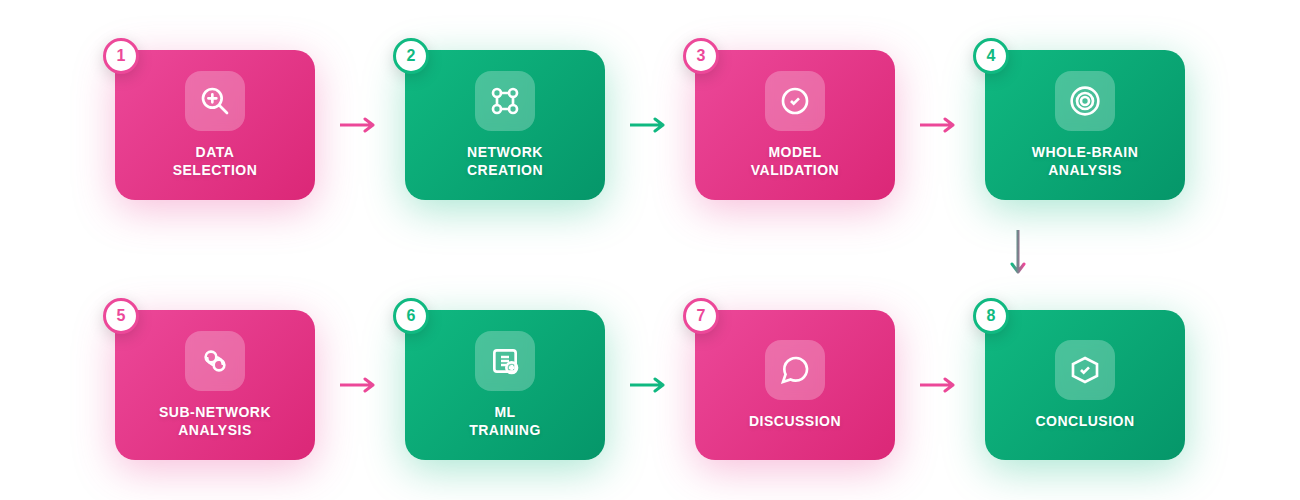
\includegraphics[width=0.83\linewidth]{../../Images/figure1_final.png}
%DIFDELCMD <  %%%
%DIFDELCMD < \caption{%
{%DIFAUXCMD
\DIFdelFL{Overview of the analytical workflow used in this study. Resting state fMRI datasets from
 the ABIDE I repository were first preprocessed using the CPAC pipeline, including standard steps
 such as motion correction, spatial normalization, and temporal filtering. The preprocessed volumes
 were then parcellated into 200 regions of interest using the CC200 atlas, yielding a regional time
 series for each participant. For every region, the fractional amplitude of low frequency fluctuations
 (fALFF) was computed, and these values were binarized to define nodal activity states distinguishing
 relatively high from relatively low intrinsic activity. Pairwise functional connectivity between
 regions was estimated from the regional BOLD time series and converted into a signed adjacency
 matrix that captures the sign of the interaction between each pair of regions. Nodal states and
 signed links were combined within the coevolutionary balance framework to compute coevolutionary
 energy at different scales. Global and local graph efficiency were computed from the absolute-value
 weighted FC matrix. To mitigate multi-site batch effects, ComBat harmonization was applied to the
 derived network features prior to statistical analysis. Null networks were generated by randomizing
 nodal states or link signs while preserving the underlying graph topology, and group comparisons
 between ASD and TD adults were carried out on the resulting measures. Energy-derived features were
 subsequently used as input to machine learning classifiers. All analyses were repeated using both
 GSR-based and no-GSR (CompCor) preprocessing pipelines.}}
 %DIFAUXCMD
%DIFDELCMD < \label{fig:flowchart}
%DIFDELCMD < \end{figure}
%DIFDELCMD < %%%
\DIFdelend \DIFaddbegin \DIFadd{We retain the original hierarchy of questions: alignment against randomized
states, whole-network configuration and energy comparisons, intra- and
inter-network comparisons, relationships with complementary network measures,
clinical correlations and partial least squares, and classification. GSR/no-GSR
comparisons are carried through each level. The revised analysis changes the
measurement and validation definitions where the original records required
clarification, while retaining these scientific questions rather than replacing
them with a different study.
}\DIFaddend 

\section*{Results}
\DIFaddbegin \subsection*{\DIFadd{Participant and measurement scope}}\linelabel{lin:participants}
\DIFadd{Figure~\ref{fig:workflow} separates demographic eligibility, feature availability, and
site-adjusted inference. Table~\ref{tab:demographics} distinguishes the 140 eligible participants from the 136 modeled
participants. The nine-site model includes an ASD-only site, CALTECH ($n=9$);
its diagnosis effect is identified through the remaining mixed-diagnosis sites,
under the common-effect regression assumption. Broader-181 and full-200 designs
have 101 (47/54) and 64 (30/34) adjusted-model participants, respectively.
}\DIFaddend 

\DIFdelbegin \subsection*{\DIFdel{Null-model validation of coevolutionary energy}}
%DIFAUXCMD
\DIFdelend \DIFaddbegin \paperfigure{Fig1}{Participant flow and derivative-based analysis}{The requested pool contains 182 adult-source participants. Age and observed IQ eligibility yields 140 male participants; all share 106 coverage-qualified nodes. Raw adjusted group models include 136 participants after excluding sites with fewer than three retained participants. Classification and individual null analyses retain all 140. MRI preprocessing and voxelwise fALFF computation occurred upstream.}{fig:workflow}
\DIFaddend 


\DIFdelbegin \DIFdel{We first asked whether the empirical coevolutionary energies observed in ASD and TD networks reflect
non-trivial alignment between binarized fALFF states and signed functional connectivity}\DIFdelend \DIFaddbegin \begin{table}[H]
\centering\small
\caption{\textbf{Participant characteristics in the two primary analysis samples.}}\label{tab:demographics}
\begin{tabular}{llrlll}
\toprule
Sample & Group & N & Age, years & FIQ & Mean FD, mm \\
\midrule
Eligible & ASD & 69 & 22.23 (3.42) & 111.23 (12.85) & 0.083 (0.045) \\
Eligible & Control & 71 & 23.00 (3.35) & 115.63 (10.98) & 0.074 (0.032) \\
Adjusted model & ASD & 67 & 22.16 (3.42) & 111.22 (12.77) & 0.081 (0.044) \\
Adjusted model & Control & 69 & 22.86 (3.30) & 115.66 (11.14) & 0.073 (0.032) \\
\bottomrule
\end{tabular}
\begin{flushleft}\footnotesize
Continuous values are mean (SD). All participants were recorded male. Eligibility is age 18--30 inclusive and observed FIQ $>80$. No handedness restriction or missing-IQ imputation is applied. The adjusted-model subset excludes four participants at sites with fewer than three eligible participants.
\end{flushleft}
\end{table}


\subsection*{\DIFadd{Null-model comparisons of coevolutionary alignment}}\linelabel{lin:results_null}
\paragraph*{\DIFadd{Male-control baseline.}}
\DIFadd{We first examined the 71 eligible male controls as a separate non-autistic
baseline}\DIFaddend , rather than \DIFdelbegin \DIFdel{arising from incidental combinations of activity and connectivity. After unified outlier removal
based on Tukey's interquartile range (IQR) applied to whole-brain coevolutionary energy (see
Methods), 78 ASDand 86 TD participants remained for null-model analyses. }%DIFDELCMD < 

%DIFDELCMD < %%%
\DIFdel{For each subject,we generated a topology-preserving null ensemble by repeatedly randomizing node
states and edge signs while keeping the underlying weighted adjacency matrix fixed. We then computed
the difference between the empirical whole-brain energy and the mean null energy for that subject. The distributions of these difference scores did not deviate from normality in either group
(Shapiro--Wilk: ASD $W = 0.992$, $p = 0.87$; TD $W = 0.989$, $p = 0.81$), supporting the use
of paired $t$-tests for this specific comparison}\DIFdelend \DIFaddbegin \DIFadd{pooling them with ASD}\DIFaddend . \DIFdelbegin %DIFDELCMD < 

%DIFDELCMD < %%%
\DIFdel{Paired-sample comparisons showed that empirical networks had substantially more negative
coevolutionary energy than their corresponding null ensembles in both groups (ASD: $t(89) = -4.12$, $p = 7.5 \times 10^{-5}$; TD: $t(91) = -3.98$, $p = 1.2 \times 10^{-4}$) . Wilcoxon signed-rank
tests yielded convergent results (ASD: $W = 1024$, $p = 9.1 \times 10^{-5}$; TD: $W = 1008$,
$p = 1.6 \times 10^{-4}$; Table~\ref{tab:null_model_validation}).
These findings confirm that the
observed coevolutionary energies capture genuine large-scale organization beyond what would be
expected from random combinations of binarized fALFF states and signed connectivity.}%DIFDELCMD < 

%DIFDELCMD < %%%
\subsection*{\DIFdel{Whole-brain coevolutionary energy and motif composition}}
%DIFAUXCMD
%DIFDELCMD < 

%DIFDELCMD < %%%
\paragraph*{\DIFdel{Adaptive statistical approach.}}
%DIFAUXCMD
\DIFdel{For each of the 92 features tested across all analyses (whole-brain, intra-network, }\DIFdelend \DIFaddbegin \DIFadd{Each control contributes 1,000
state permutations per pipeline and null scheme. Mean empirical $H$ is $-91.39$
with GSR and $-66.62$ without GSR. The corresponding unrestricted null means
are 1.49 }\DIFaddend and \DIFdelbegin \DIFdel{inter-network
metrics, including global and local graph efficiency), we conducted Shapiro--Wilk normality tests
for the
ASD and TD distributions separately, and Levene's test for homogeneity of variance. The
decision rule was pre-specified: if both groups passed Shapiro--Wilk ($p > 0.05$), an
independent-samples $t$-test was applied; if either group failed, Mann--Whitney $U$ was used; and
if both groups were normal but Levene's test indicated unequal variances, Welch's $t$-test was
applied.
The normality criterion was evaluated for each feature before group differences were
inspected, so that test selection was determined by the distributional properties of the data rather
than by the resulting $p$-values}\DIFdelend \DIFaddbegin \DIFadd{17.11; mean empirical-minus-null differences are $-92.88$ and
$-83.73$, with descriptive site-bootstrap 95\% intervals of $-103.90$ to
$-79.89$ and $-89.79$ to $-77.66$, respectively}\DIFaddend .

\DIFdelbegin \DIFdel{The normality results, summarized in Supplementary Table~\ref{tab:supp_normality}, show that the vast majority of features violate normality in at least one group: all 8 whole-brain features and all 21 intra-network features were non-normal in both groups (Shapiro--Wilk $p < 0.05$), and 51
of the 63 inter-network features were non-normal in at least one group. Across all 92 features,
Mann--Whitney $U$ was the appropriate test for the large majority (about 87\%), standard $t$-tests for 10 (11\%), }\DIFdelend \DIFaddbegin \DIFadd{With network/hemisphere-constrained states, the null means are $-41.35$ }\DIFaddend and
\DIFdelbegin \DIFdel{Welch's $t$-test for 2 }\DIFdelend \DIFaddbegin \DIFadd{$-18.85$, and the empirical-minus-null differences are $-50.04$ }\DIFaddend (\DIFdelbegin \DIFdel{2\%). This distribution reflects the heavy-tailed and skewed character of
energy-based and connectivity measures after ComBat harmonization, and accounts for the
predominance of non-parametric testing throughout the analyses. }%DIFDELCMD < 

%DIFDELCMD < %%%
\DIFdel{We compared whole-brain coevolutionary metrics between ASD }\DIFdelend \DIFaddbegin \DIFadd{95\% interval
$-54.14$ to $-44.03$) }\DIFaddend and \DIFdelbegin \DIFdel{TD adults using the cleaned sample
obtained after IQR-based outlier removal on whole-brain energy (see Table~\ref{tab:demographics}
for final group sizes).
In this binarized formulation, }\DIFdelend \DIFaddbegin \DIFadd{$-47.76$ ($-53.11$ to $-42.16$).
Table~\ref{tab:nulls} and Fig.~\ref{fig:null} show these comparisons;
individual null $z$-scores are plotted in S1 Appendix.
All 71 controls in each pipeline have empirical $H$ below their unrestricted
null mean. Under the blocked null, this holds for 69/71 with GSR and 67/71
without GSR. After exploratory BH correction over all 560 individual participant/pipeline/null
comparisons, the numbers with lower-tail $q<.05$ are 61/71 and 64/71 for the
unrestricted null and 36/71 and 50/71 for the blocked null (GSR/no-GSR).
}

\paperfigure{Fig2}{Empirical alignment relative to individual null means}{Each point is empirical H minus the participant-specific mean of 1,000 permutations. Panels separate pipelines and unrestricted versus network/hemisphere-blocked reassignment. ASD is magenta and controls dark green. FC is fixed; these are state permutations, not topology-rewired graphs. Negative values indicate lower empirical H than the specified null expectation.}{fig:null}


\DIFadd{Thus empirical control state assignments tend to align with their own FC more
strongly than }\DIFaddend the \DIFdelbegin \DIFdel{global Hamiltonian $H(G)$, the fraction
of links whose sign agrees with the product of nodal states (Agreement),
and the fractions of links
falling into different imbalance categories (Imbalanced Same, Imbalanced Opposite)jointly
characterize how nodal fALFF states co-align with signed functional connectivity. All analyses were
performed on ComBat-harmonized features (see Methods).
}\DIFdelend \DIFaddbegin \DIFadd{randomized assignments under both specified nulls, with
substantial dependence on the constraints. This is evidence about the chosen
alignment statistic and randomizations, not proof of dynamical equilibrium,
a comparison with topology-rewired graphs, or an autism-specific effect.
}\DIFaddend 

\DIFdelbegin \DIFdel{At the level of the global Hamiltonian, ASD networks showed nominally more negative whole-brain
energy than TD participants (ASD: $-139.7 \pm 78.7$; TD: $-118.8 \pm 76.2$), in the direction of a
stronger alignment between nodal activity states and signed connectivity.
This difference, however,
did not survive FDR correction across the eight whole-brain features (Mann--Whitney $U$, uncorrected
$p = 0.048$, $p_{\mathrm{FDR}} = 0.19$; Table~\ref{tab:assumptions_and_tests}). }\DIFdelend \DIFaddbegin \begin{table}[H]
\centering\small
\caption{\textbf{Empirical alignment against state-permutation null configurations.}}\label{tab:nulls}
\begin{tabular}{lllrrrrr}
\toprule
Group & Pipeline & Null & N & Mean H & Mean null H & Mean z & q<.05 count \\
\midrule
ASD & GSR & B & 69 & -93.173 & -43.546 & -2.331 & 40 \\
ASD & GSR & U & 69 & -93.173 & 1.611 & -4.705 & 61 \\
ASD & noGSR & B & 69 & -64.250 & -20.849 & -2.591 & 46 \\
ASD & noGSR & U & 69 & -64.250 & 16.297 & -4.917 & 60 \\
Control & GSR & B & 71 & -91.392 & -41.354 & -2.313 & 36 \\
Control & GSR & U & 71 & -91.392 & 1.486 & -4.690 & 61 \\
Control & noGSR & B & 71 & -66.618 & -18.854 & -2.760 & 50 \\
Control & noGSR & U & 71 & -66.618 & 17.109 & -5.159 & 64 \\
\bottomrule
\end{tabular}
\begin{flushleft}\footnotesize
U: unrestricted state permutations; B: network/hemisphere-blocked permutations. Each person has 1,000 permutations under each scheme. BH correction here spans all 560 person/pipeline/null comparisons; the counts do not test an ASD--control difference.
\end{flushleft}
\end{table}

\DIFaddend 

\DIFdelbegin \DIFdel{Motif-based measures showed the same directional pattern but likewise did not survive correction.
The proportion of imbalanced-same links was nominally lower in ASD (ASD: $0.256$; TD: $0.258$;
$t$-test, $p = 0.047$, $p_{\mathrm{FDR}} = 0.19$) and the proportion of agreement links nominally
higher (ASD: $0.241$; TD: $0.240$; $t$-test}\DIFdelend \DIFaddbegin \paragraph*{\DIFadd{ASD and across-diagnosis summaries.}}
\DIFadd{All 140 participants per pipeline have finite null scores under both randomizations.
Within ASD alone ($n=69$), mean unrestricted $z$ is $-4.705$/$-4.917$
(GSR/no-GSR)}\DIFaddend , \DIFdelbegin \DIFdel{$p = 0.070$, $p_{\mathrm{FDR}} = 0.19$). Disagreement
and imbalanced-opposite proportions did not differ between groups ($p = 0.68$ }\DIFdelend and \DIFdelbegin \DIFdel{$p = 0.82$).
Whole-brain bipolarity ($0.626$ vs.\ $0.627$; $p = 0.53$)
}\DIFdelend \DIFaddbegin \DIFadd{blocked mean $z$ is $-2.331$/$-2.591$. With exploratory
BH across all 560 participant/pipeline/null comparisons, the ASD lower-tail
$q<.05$ counts are 61/69 and 60/69 for unrestricted states, and 40/69 }\DIFaddend and
\DIFdelbegin \DIFdel{global and local graph efficiency
(both $p > 0.99$) showed no group difference.
}\DIFdelend \DIFaddbegin \DIFadd{46/69 for blocked states. These complements retain the original ASD as well
as control null question and do not test diagnosis differences.
The corresponding across-diagnosis summaries are retained for completeness.
Mean unrestricted $z$ is $-4.70$/$-5.04$ (GSR/no-GSR), compared with
$-2.32$/$-2.68$ under network/hemisphere blocks. These values show dependence on
the randomization scheme, not diagnosis discrimination or preservation of full
spatial structure. Individual scores and probabilities are in S2 Data.
}\DIFaddend 



\DIFdelbegin \DIFdel{Together, the harmonized GSRdata reveal consistent but weak, uncorrected trends---more negative
energy and a modest redistribution of motifs toward agreement and away from imbalanced-same links in
ASD---but no whole-brain feature reaches FDR significance. The direction of these trends matches that
seen before harmonization, while their magnitude and significance are substantially reduced (see
``Effect of site harmonization'' below). Quantitative values for all whole-brain metrics are provided
in Supplementary Table~}\DIFdelend \DIFaddbegin \subsection*{\DIFadd{Whole-network coevolutionary energy and motif composition}}
\DIFadd{Primary adjusted coefficients are 1.432 with GSR (95\% CI $-17.173$ to 20.038,
$p=.879$) and 2.056 without GSR (95\% CI $-12.387$ to 16.499, $p=.779$);
both Holm-adjusted $p=1.000$ (Table~\ref{tab:primary}, Fig.~\ref{fig:global}).
No valid secondary group test survives its specified correction in any raw or
ComBat design. The trimming sensitivities likewise do not identify a corrected
$H$ difference. Larger-node results are in }\DIFaddend S1 \DIFdelbegin \DIFdel{, and their distributions are illustrated in Fig~\ref{fig:enter-label}.
}\DIFdelend \DIFaddbegin \DIFadd{Appendix.
}\DIFaddend 

\DIFdelbegin %DIFDELCMD < \begin{figure}[H]
%DIFDELCMD <     \centering
%DIFDELCMD <     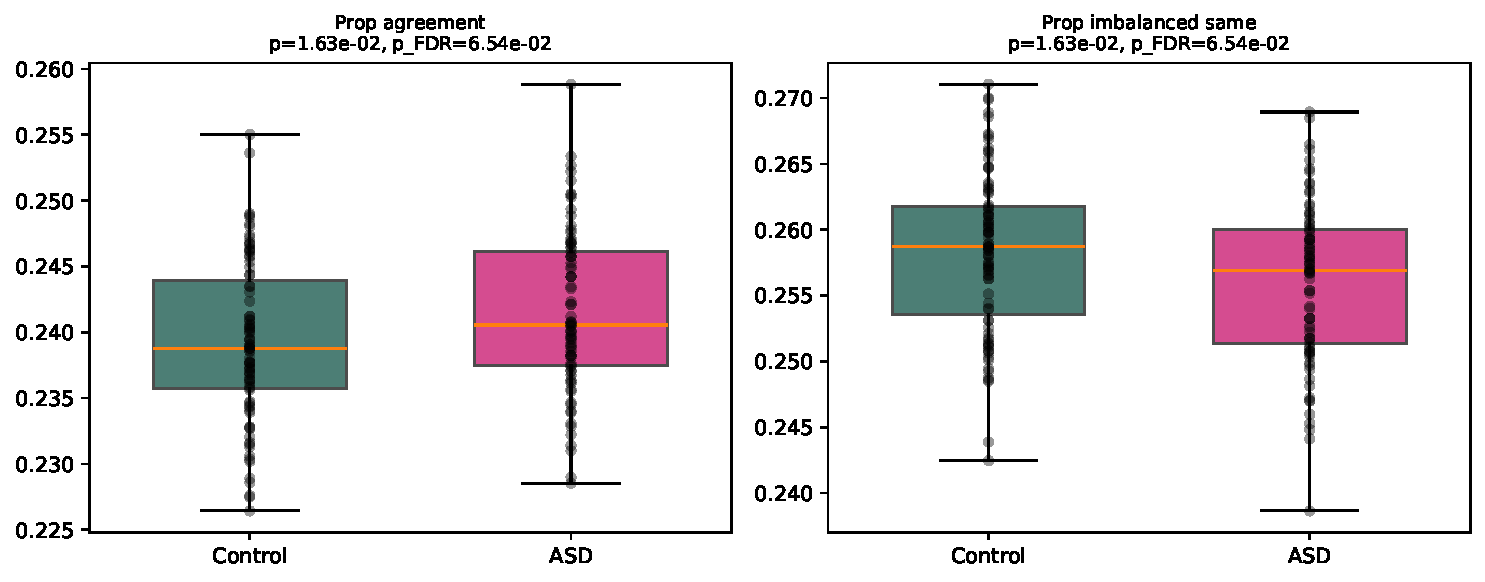
\includegraphics[width=0.75\linewidth]{../../Images/Whole_significant_GSR.pdf}
%DIFDELCMD <     %%%
%DIFDELCMD < \caption{%
{%DIFAUXCMD
\DIFdelFL{Whole-brain coevolutionary metrics for autistic (ASD) and typically developing (TD)
    adults after ComBat harmonization. Each panel shows the distribution of a global measure derived
    from the signed functional network: (top row, from left to right) total coevolutionary energy,
    the proportion of imbalanced-same links, and the proportion of agreement links; (bottom row,
    from left to right) the proportion of disagreement links and the proportion of
    imbalanced-opposite links. Boxplots display the median (central line), interquartile range
    (box), and 1.5~$\times$~IQR whiskers, with individual participants overlaid as jittered points
    (magenta/pink for ASD, green for controls). Raw and FDR-corrected $p$-values are shown above
    each panel. The panels shown are the whole-brain metrics with the smallest group-comparison
    $p$-values (proportion of agreement and imbalanced-same links); both showed only weak,
    uncorrected trends in ASD (more agreement and fewer imbalanced-same links) that did not survive
    FDR correction ($p_{\mathrm{FDR}} > 0.05$). Consistent with Table~\ref{tab:assumptions_and_tests},
    no whole-brain coevolutionary metric differed significantly between groups after harmonization.}}
    %DIFAUXCMD
%DIFDELCMD < \label{fig:enter-label}
%DIFDELCMD < \end{figure}
%DIFDELCMD < %%%
\DIFdelend \DIFaddbegin \paperfigure{Fig3}{Global feature distributions in both processing pipelines}{Points and boxes describe the untrimmed 140-person feature cohort: 69 ASD and 71 controls. ASD is magenta and controls dark green. Seven available global quantities include H, four pairwise configuration proportions and two absolute-weight efficiencies. Adjusted inference uses 136 participants; distribution overlap is not an equivalence test.}{fig:global}
\DIFaddend 


\DIFdelbegin \subsection*{\DIFdel{Network-specific coevolutionary metrics}}
%DIFAUXCMD
%DIFDELCMD < 

%DIFDELCMD < %%%
\DIFdel{We next asked whether coevolutionary balance differs between ASD and TD within canonical large-scale
networks. Using the Yeo 7-network parcellation }%DIFDELCMD < \cite{Yeo2011}%%%
\DIFdel{, each CC200 parcel was assigned to
the network with maximal Dice overlap, and for every subject we summarized edges confined to a given
network $u$ in three intra-network metrics: (i) the mean Fisher-$z$ transformed functional
connectivity (AvgWeight$_u$), (ii) the mean fALFF-aligned connectivity (AvgFalffW$_u = \langle
w_{ij} s_i s_j \rangle$ over $i,j \in u$),
and (iii) the intra-network coevolutionary energy
contribution $E_u$, computed as the Hamiltonian (see Methods, Eq.~\ref{eq:hamiltonian}) restricted
to edges within network $u$.
}\DIFdelend \DIFaddbegin \begin{table}[H]
\centering\small
\caption{\textbf{Adjusted diagnosis coefficients for primary-network H.}}\label{tab:primary}
\begin{tabular}{llrrlrr}
\toprule
Pipeline & Model & N & Coefficient & 95\% CI & p & Holm p \\
\midrule
GSR & Raw adjusted & 136 & 1.432 & -17.17, 20.04 & 0.879 & 1.000 \\
GSR & ComBat & 136 & 1.139 & -17.15, 19.42 & 0.902 & 1.000 \\
GSR & Pooled trim & 135 & -2.613 & -19.56, 14.34 & 0.761 & 1.000 \\
noGSR & Raw adjusted & 136 & 2.056 & -12.39, 16.50 & 0.779 & 1.000 \\
noGSR & ComBat & 136 & 2.247 & -11.81, 16.30 & 0.752 & 1.000 \\
noGSR & Pooled trim & 135 & 3.500 & -10.77, 17.77 & 0.628 & 1.000 \\
\bottomrule
\end{tabular}
\begin{flushleft}\footnotesize
Coefficients compare ASD with controls, adjusting for site, age, FIQ and mean FD. HC3 intervals use a t reference. Holm correction covers the two pipelines within each model version. ComBat and pooled trimming are exploratory sensitivities.
\end{flushleft}
\end{table}

\DIFaddend 

\DIFdelbegin \DIFdel{All intra-network comparisons used the unified outlier-cleaned and ComBat-harmonized sample (see
Methods) and the same adaptive statistical pipelineas for the whole-brain metrics. Table~\ref{tab:network_results} summarizes group means and $p$-values for the intra-network metrics.}\DIFdelend \DIFaddbegin \DIFadd{Figure~\ref{fig:global} displays all seven valid global quantities for
the untrimmed 140-person feature cohort. Within- and between-network
effect heatmaps below show all prespecified cortical blocks rather than selecting
nominally significant examples.
}\DIFaddend 

\DIFdelbegin \DIFdel{None of the intra-network metrics reached significance after FDR correction, and---unlike the
pre-harmonization analysis---none reached even nominal (uncorrected) significance.
The smallest
$p$-value was for Salience}\DIFdelend \DIFaddbegin \DIFadd{All six ComBat design}\DIFaddend /\DIFdelbegin \DIFdel{Ventral Attention average connectivity (ASD lower than TD; $t$-test}\DIFdelend \DIFaddbegin \DIFadd{pipeline pairs complete with finite, changed feature values.
Primary descriptive site partial $R^2$ decreases from .056 to .004 with GSR and
from .047 to .005 without GSR. Maximum primary leverage is .352; maximum Cook's
distance is .080 or smaller across these four raw/ComBat fits. These checks do
not establish perfect harmonization or independence of participants within sites.
Excluding CALTECH yields 127 participants (58 ASD}\DIFaddend , \DIFdelbegin \DIFdel{$p = 0.064$}\DIFdelend \DIFaddbegin \DIFadd{69 controls) at eight sites;
raw adjusted coefficients remain imprecise (GSR: 1.115}\DIFaddend , \DIFdelbegin \DIFdel{$p_{\mathrm{FDR}} = 0.57$), followed by SomatoMotor and Limbic intra-network energy
(both $p > 0.10$). In the harmonized data, therefore,
the intra-network analyses provide no evidence
for spatially circumscribed shifts in coevolutionary energy within individual Yeo networks. The few
intra-network differences that appeared nominally significant before harmonization (e.g.\ the Visual
network)did not persist once site effects were removed, }\DIFdelend \DIFaddbegin \DIFadd{95\% CI $-17.531$ to
19.762; no-GSR: 1.660, 95\% CI $-12.775$ to 16.096; both Holm $p=1.000$).
}

\DIFadd{Primary unadjusted Hedges' $g$ is $-.024$ (bootstrap 95\% CI $-.384$ to .315)
with GSR and .072 ($-.268$ to .412) without GSR. Approximate two-sample 80\%-power
minimum detectable $d$ is .484 at $\alpha=.05$, or .534 at $\alpha=.025$.
Equivalence tests are inconclusive ($p=.193$ }\DIFaddend and \DIFdelbegin \DIFdel{the largest remaining trends are summarized in Table~\ref{tab:network_results} for completeness}\DIFdelend \DIFaddbegin \DIFadd{.223). Nonsignificant contrasts
therefore do not demonstrate absence of a meaningful diagnosis effect}\DIFaddend .

\DIFdelbegin %DIFDELCMD < \begin{figure}[H]
%DIFDELCMD <  \centering
%DIFDELCMD <  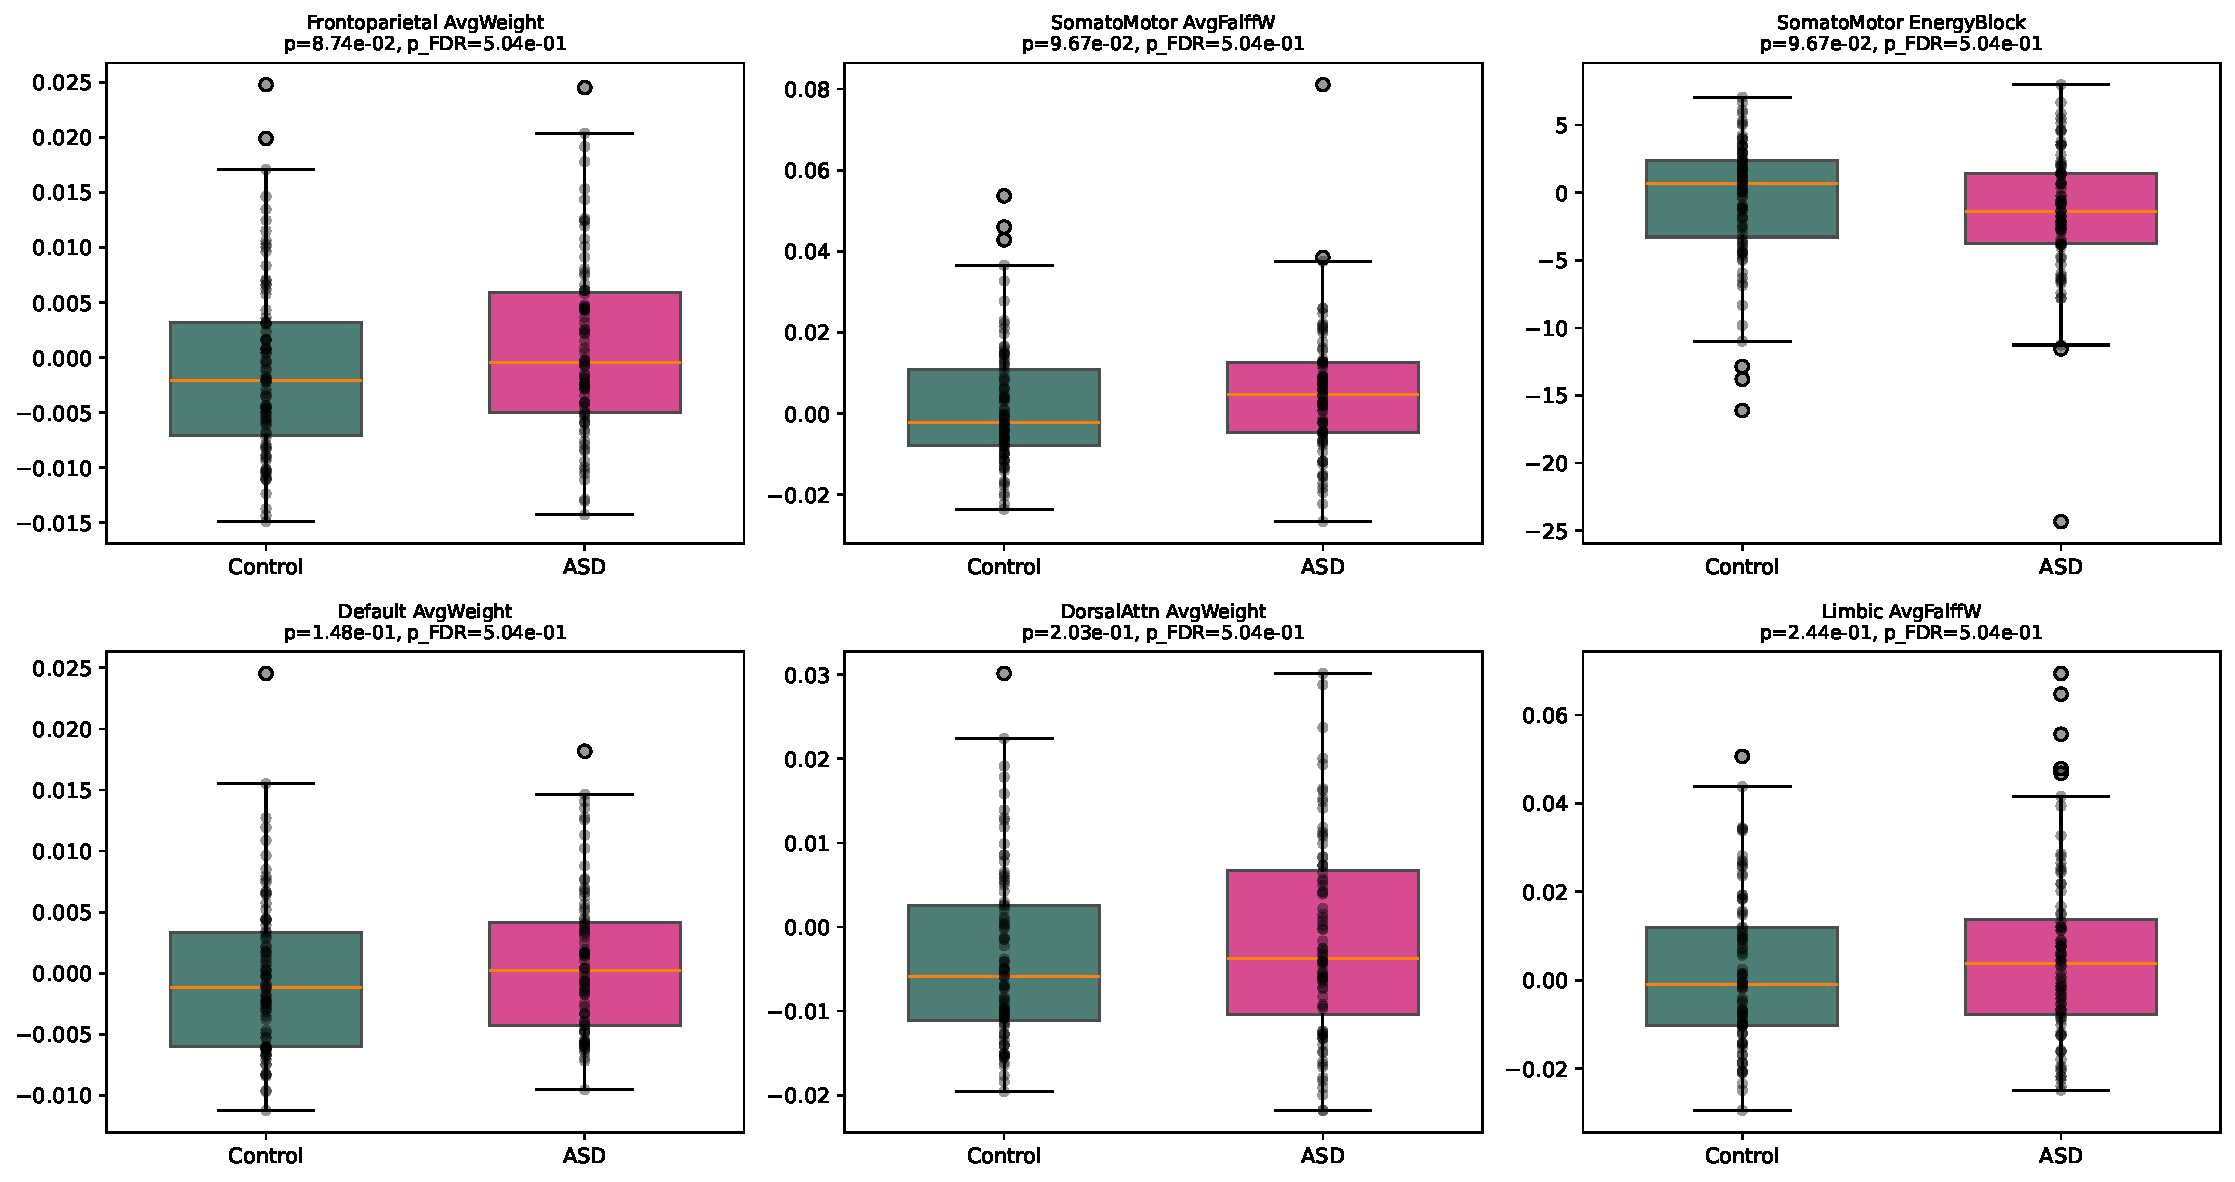
\includegraphics[width=0.85\linewidth]{../../Images/Intra_significant_GSR.pdf}
%DIFDELCMD <  %%%
%DIFDELCMD < \caption{%
{%DIFAUXCMD
\DIFdelFL{Distributions of the largest intra-network trends between ASD and TD adults under the
 harmonized GSR pipeline. Boxplots display the metrics with the smallest group-comparison
 $p$-values (Table~\ref{tab:network_results}). None reached nominal or FDR-corrected significance
 after harmonization; panels are shown for completeness.}}
 %DIFAUXCMD
%DIFDELCMD < \label{fig:subnetworks_FDR-raw}
%DIFDELCMD < \end{figure}
%DIFDELCMD < 

%DIFDELCMD < %%%
\subsection*{\DIFdel{Inter-network connectivity and energy}}
%DIFAUXCMD
%DIFDELCMD < 

%DIFDELCMD < %%%
\DIFdel{To extend the intra-network analyses, we next examined how coevolutionary balance and connectivity
are organized between large-scale systems. Interactions were quantified for each unordered pair
$(u,v)$ of the seven Yeo resting-state networks }%DIFDELCMD < \cite{Yeo2011}%%%
\DIFdel{, yielding 21 distinct network pairs .
After unified outlier removal and harmonization (see Methods), 78 autistic
and 86 TD participants remained for this analysis.
}%DIFDELCMD < 

%DIFDELCMD < %%%
\DIFdel{For every network pair $(u,v)$ we computed three complementary quantities that capture different
aspects of between-network coupling: average functional connectivity ($\mathrm{AvgWeight}_{uv}$),
fALFF-aligned connectivity ($\mathrm{AvgFalffW}_{uv}$), and inter-network coevolutionary energy
($E_{uv}$),
as defined in the Methods. Group differences in each metric were assessed using the
adaptive statistical pipeline(Shapiro--Wilk-guided $t$-test or Mann--Whitney $U$) applied
separately to every network pair and measure. To control for multiple comparisons across the 63
inter-network metrics (21 pairs $\times$ 3 measures),
we applied Benjamini--Hochberg FDR correction. }%DIFDELCMD < 

%DIFDELCMD < %%%
\DIFdel{No inter-network metric survived FDR correction at $\alpha = 0.05$. The strongest effect was for
SomatoMotor--Frontoparietal average connectivity, which was higher in ASD than TD (ASD $0.0037$, TD
$0.0008$; $t$-test}\DIFdelend \DIFaddbegin \subsection*{\DIFadd{Network-specific coevolutionary metrics}}\linelabel{lin:results_intra}
\DIFadd{Table~\ref{tab:intra} reports block-energy contrasts. We retain the original within-network question: whether ASD and control
participants differ in mean FC (AvgWeight)}\DIFaddend , \DIFdelbegin \DIFdel{$p = 0.0011$}\DIFdelend \DIFaddbegin \DIFadd{mean state-weighted FC (AvgFalffW)}\DIFaddend ,
\DIFdelbegin \DIFdel{$p_{\mathrm{FDR}} = 0.069$). Additional uncorrected effects
involved average connectivity between attention, control, and somatomotor systems: SomatoMotor--
Salience}\DIFdelend \DIFaddbegin \DIFadd{or block Hamiltonian contribution (EnergyBlock) within each of the seven Yeo
systems. The primary graph permits 18 tests per pipeline; three within-limbic
quantities are unavailable because only one limbic node remains. All available
blocks are shown in Fig.~\ref{fig:intra}, with complete estimates in S2.
No comparison survives BH across the 36 pipeline}\DIFaddend /\DIFdelbegin \DIFdel{VentAttn ($p = 0.003$}\DIFdelend \DIFaddbegin \DIFadd{within-network tests. In GSR,
the smallest raw probability is .073. Without GSR, somatomotor mean FC is
nominally lower in ASD (coefficient $-.0683$}\DIFaddend , \DIFdelbegin \DIFdel{$p_{\mathrm{FDR}} = 0.095$), DorsalAttn--Salience/VentAttn
($p = 0.008$}\DIFdelend \DIFaddbegin \DIFadd{$p=.0371$)}\DIFaddend , \DIFdelbegin \DIFdel{$p_{\mathrm{FDR}} = 0.16$), and DorsalAttn--Frontoparietal ($p = 0.015$}\DIFdelend \DIFaddbegin \DIFadd{as is default-network
mean FC ($-.0519$}\DIFaddend , \DIFdelbegin \DIFdel{$p_{\mathrm{FDR}} = 0.24$), all showing higher inter-network connectivity in ASD, together with
Visual--Default inter-network energy ($p = 0.047$,
$p_{\mathrm{FDR}} = 0.59$). Table~\ref{tab:internetwork_new} lists the inter-network metrics with the smallest
$p$-values. }%DIFDELCMD < 

%DIFDELCMD < %%%
\DIFdel{These trends suggest that, although no effect reaches the FDR threshold, the most consistent
direction in the harmonized data is one of mildly increased between-system connectivity in ASD,
particularly among somatomotor, attention, and frontoparietal control networks. As none survives
correction, they should be regarded as hypotheses for larger samples rather than established
findings}\DIFdelend \DIFaddbegin \DIFadd{$p=.0432$); both become $q=.392$ and are not corrected findings}\DIFaddend .

\DIFdelbegin %DIFDELCMD < \begin{figure}[H]
%DIFDELCMD <  \centering
%DIFDELCMD <  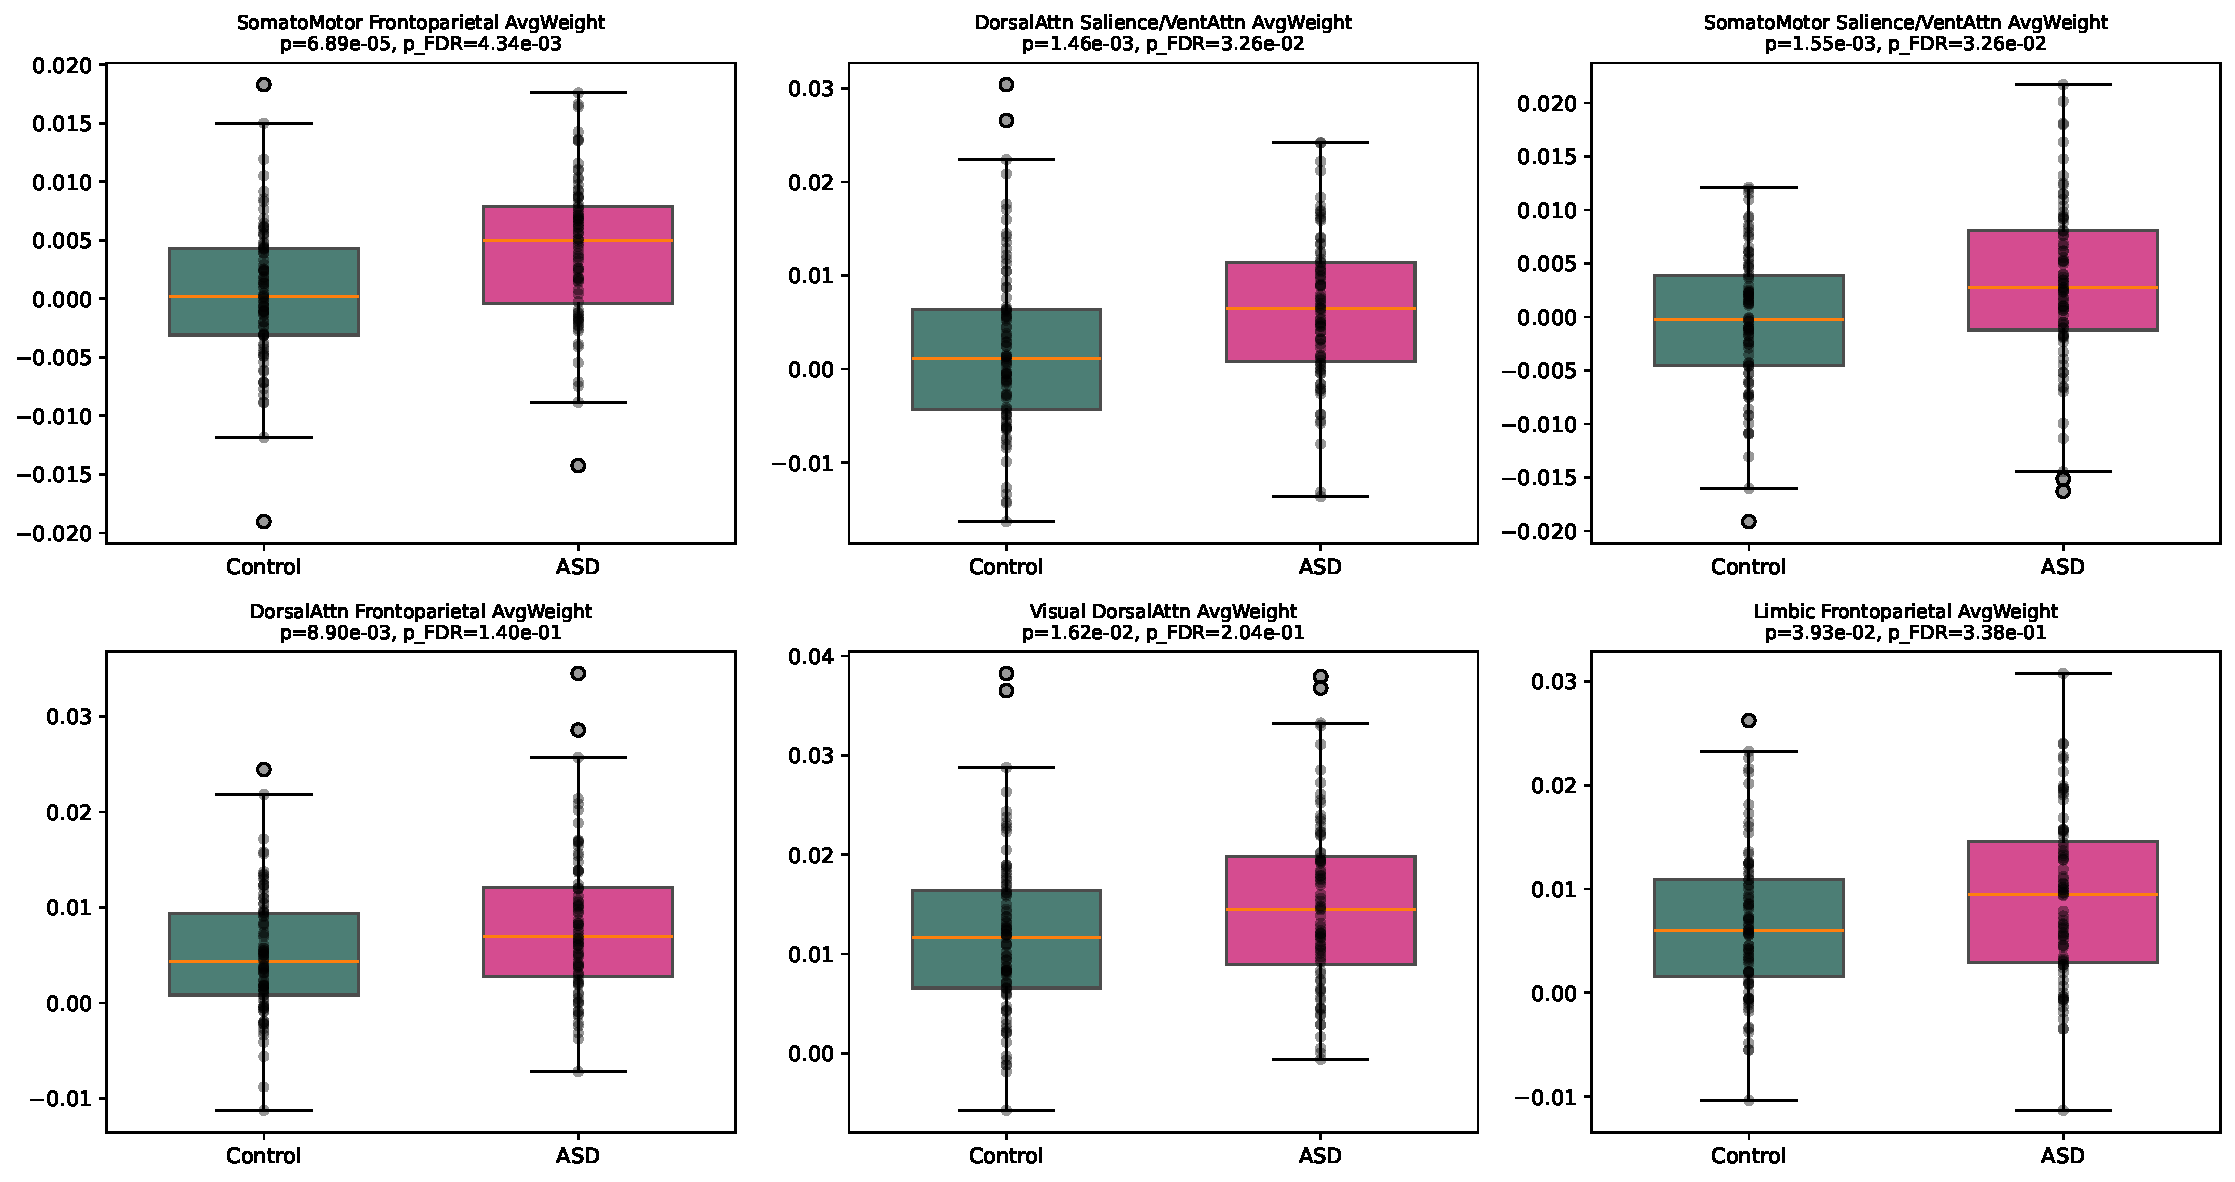
\includegraphics[width=0.95\linewidth]{../../Images/Inter_significant_GSR.pdf}
%DIFDELCMD <  %%%
%DIFDELCMD < \caption{%
{%DIFAUXCMD
\DIFdelFL{Distributions of the inter-network metrics with the smallest group-comparison $p$-values
 between ASD and TD adults under the harmonized GSR pipeline (Table~\ref{tab:internetwork_new}). The
 strongest effect is SomatoMotor--Frontoparietal average connectivity ($p_{\mathrm{FDR}} = 0.069$).
 None survived FDR correction; effects are exploratory.}}
 %DIFAUXCMD
%DIFDELCMD < \label{fig:inter_network}
%DIFDELCMD < \end{figure}
%DIFDELCMD < %%%
\DIFdelend \DIFaddbegin \begin{table}[H]
\centering\small
\caption{\textbf{Within-network energy diagnosis coefficients.}}\label{tab:intra}
\begin{tabular}{lllllll}
\toprule
Network & GSR beta & GSR 95\% CI & GSR q & No-GSR beta & No-GSR 95\% CI & No-GSR q \\
\midrule
VIS & 3.451 & -0.51, 7.41 & 0.392 & 6.746 & -0.27, 13.76 & 0.392 \\
SM & -2.877 & -6.74, 0.99 & 0.469 & -2.712 & -8.88, 3.46 & 0.830 \\
DA & 0.584 & -0.83, 2.00 & 0.830 & 0.782 & -1.47, 3.03 & 0.875 \\
SV & -0.301 & -2.37, 1.77 & 0.875 & -0.496 & -3.38, 2.39 & 0.875 \\
LIM & -- & -- & -- & -- & -- & -- \\
FP & -0.620 & -2.64, 1.40 & 0.875 & -0.399 & -3.88, 3.08 & 0.875 \\
DMN & 0.182 & -1.46, 1.82 & 0.875 & 0.473 & -2.16, 3.10 & 0.875 \\
\bottomrule
\end{tabular}
\begin{flushleft}\footnotesize
Raw adjusted models use 136 participants. BH spans both pipelines and all available within-network measures (36 tests). Limbic energy is unavailable because only one node is assigned. VIS: visual; SM: somatomotor; DA: dorsal attention; SV: salience/ventral attention; LIM: limbic; FP: frontoparietal; DMN: default mode. Other block measures are shown in Fig.~\ref{fig:intra} and S2 Data.
\end{flushleft}
\end{table}

\DIFaddend 


\DIFdelbegin \subsection*{\DIFdel{Correlation analysis of network metrics with behavioral scores}}
%DIFAUXCMD
\DIFdelend \DIFaddbegin \paperfigure{Fig4}{Within-network diagnosis comparisons}{Cells show the raw adjusted diagnosis coefficient divided by its HC3 standard error for mean FC, mean state-weighted FC and block energy. Both pipelines use 136 participants. Gray within-limbic cells are unavailable because only one limbic node remains. None of the 36 valid tests survives BH correction. Color encodes signed t statistics, not significance.}{fig:intra}
\DIFaddend 


\DIFdelbegin \DIFdel{We next examined how whole-brain, subnetwork, and }\DIFdelend \DIFaddbegin \subsection*{\DIFadd{Inter-network connectivity and energy}}\linelabel{lin:results_inter}
\DIFadd{Table~\ref{tab:inter} reports all mean-FC contrasts. We also retain all 21 unordered network pairs and all three original measures,
yielding 63 tests per pipeline. Fig.~\ref{fig:inter} shows every block,
including nonsignificant ones. No comparison survives BH across the 126
pipeline/}\DIFaddend inter-network \DIFdelbegin \DIFdel{coevolutionary metrics relate to
clinical variation in the autistic group. Building on our initial exploratory correlations, we conducted a comprehensive analysis correlating all 92 ComBat-harmonized network features against the
five ADI-R and ADOS subscales with sufficient data: ADI-R Social Total A, ADI-R Verbal Total BV,
ADI-R Onset Total D, ADOS Total, and ADOS Communication.
Correlations were computed only in ASD participants with valid clinical scores drawn from the same
harmonized, outlier-cleaned cohort (Table~\ref{tab:demographics}); sample sizes varied by clinical
measure due to missing values (range: $n = 29$--59 per analysis). }%DIFDELCMD < 

%DIFDELCMD < %%%
\DIFdel{For each of the 460 feature--clinical score combinations (92 features $\times$ 5 clinical scores),
we estimated both Pearson 's product--moment correlation coefficient ($r$) and Spearman's rank
correlation coefficient ($\rho$), together with their exact two-tailed $p$-values. To control for
multiple comparisons, we applied Benjamini--Hochberg false discovery rate (FDR) correction
separately for the Pearson and Spearman $p$-values across all 460 }\DIFdelend tests. \DIFaddbegin \DIFadd{GSR salience/ventral-attention--limbic state-weighted
FC and its corresponding block energy are nominally different ($p=.0315$,
$q=.756$). They are proportional descriptions of the same block, not two
independent effects. No no-GSR inter-network test reaches $p<.05$; its smallest
raw probability is .0508. These results address spatially specific diagnosis
effects separately from the global Hamiltonian and the within-group associations.
}\DIFaddend 

\DIFdelbegin \DIFdel{At the uncorrected threshold of $p < 0.05$}\DIFdelend \DIFaddbegin \begin{table}[H]
\centering\small
\caption{\textbf{Between-network mean-FC diagnosis coefficients.}}\label{tab:inter}
\begin{tabular}{llrrlrr}
\toprule
Pair & GSR beta & GSR p & GSR q & No-GSR beta & No-GSR p & No-GSR q \\
\midrule
VIS--SM & -0.0059 & 0.738 & 0.893 & -0.0523 & 0.082 & 0.756 \\
VIS--DA & -0.0060 & 0.715 & 0.893 & -0.0573 & 0.051 & 0.756 \\
VIS--SV & 0.0093 & 0.466 & 0.874 & -0.0459 & 0.098 & 0.756 \\
VIS--LIM & 0.0289 & 0.228 & 0.835 & -0.0388 & 0.318 & 0.835 \\
VIS--FP & 0.0117 & 0.288 & 0.835 & -0.0381 & 0.143 & 0.756 \\
VIS--DMN & -0.0052 & 0.684 & 0.877 & -0.0531 & 0.053 & 0.756 \\
SM--DA & -0.0115 & 0.506 & 0.877 & -0.0486 & 0.139 & 0.756 \\
SM--SV & 0.0040 & 0.781 & 0.922 & -0.0324 & 0.257 & 0.835 \\
SM--LIM & -0.0110 & 0.666 & 0.877 & -0.0592 & 0.098 & 0.756 \\
SM--FP & 0.0104 & 0.472 & 0.874 & -0.0233 & 0.443 & 0.874 \\
SM--DMN & 0.0195 & 0.143 & 0.756 & -0.0243 & 0.386 & 0.859 \\
DA--SV & -0.0006 & 0.968 & 0.987 & -0.0424 & 0.168 & 0.756 \\
DA--LIM & -0.0284 & 0.307 & 0.835 & -0.0678 & 0.097 & 0.756 \\
DA--FP & -0.0010 & 0.940 & 0.987 & -0.0365 & 0.186 & 0.780 \\
DA--DMN & -0.0027 & 0.876 & 0.968 & -0.0443 & 0.155 & 0.756 \\
SV--LIM & -0.0132 & 0.587 & 0.877 & -0.0603 & 0.078 & 0.756 \\
SV--FP & -0.0123 & 0.244 & 0.835 & -0.0450 & 0.115 & 0.756 \\
SV--DMN & 0.0139 & 0.258 & 0.835 & -0.0322 & 0.273 & 0.835 \\
LIM--FP & -0.0323 & 0.186 & 0.780 & -0.0548 & 0.136 & 0.756 \\
LIM--DMN & 0.0251 & 0.335 & 0.835 & -0.0146 & 0.689 & 0.877 \\
FP--DMN & 0.0039 & 0.783 & 0.922 & -0.0294 & 0.289 & 0.835 \\
\bottomrule
\end{tabular}
\begin{flushleft}\footnotesize
Raw adjusted models use 136 participants. BH spans all three between-network measures in both pipelines (126 tests); q values therefore refer to the full family, not just this mean-FC table. Network abbreviations follow Table~\ref{tab:intra}. State-weighted FC and energy are included in Fig.~\ref{fig:inter} and S2 Data.
\end{flushleft}
\end{table}



\paperfigure{Fig5}{Between-network diagnosis comparisons}{All 21 cortical network pairs and all three block measures are shown in both pipelines. Cells show HC3 t statistics from raw adjusted models. No test survives BH across the 126 valid comparisons. Mean state-weighted FC and block energy are proportional for a fixed block and do not provide independent effects.}{fig:inter}


\subsection*{\DIFadd{Relationships between H and other network metrics}}\linelabel{lin:Hcorrelations}
\DIFadd{To preserve the original descriptive analysis, we correlate $H$ with all 87 other
available nonlegacy features within ASD and controls separately, in both pipelines.
All eligible participants are included (69 ASD/71 controls). Under the original
per-group Pearson BH convention, 26 GSR-ASD}\DIFaddend , 21 \DIFdelbegin \DIFdel{feature--clinical score pairs showed nominally
significant associations---close to the number expected by chance. None survived FDR correction at
$q < 0.05$.
The full correlation matrix is provided in Supplementary Table~\ref{tab:supp_corr_full}, and the
complete list of nominally significant associations is available in Supplementary
Table~\ref{tab:supp_corr_sig}.
}\DIFdelend \DIFaddbegin \DIFadd{GSR-control, and 12 no-GSR-ASD
associations survive $q<.05$; none survives in no-GSR controls
(Table~\ref{tab:Hcounts}). Figure~\ref{fig:Hcorrelations} restores the
original top-20 presentation, while S2 contains every test, not just ranked results.
}\DIFaddend 

\DIFdelbegin \DIFdel{Despite testing 460 feature--score pairs (92 features $\times$ 5 clinical scores with sufficient
data), no association survived FDR correction, and only 21 reached uncorrected $p < 0.05$---close to
the number expected by chance alone. Crucially, the whole-brain Hamiltonian was not associated with
symptom severity in the harmonized data (ADOS Total: $r = -0.10$, $p = 0.47$, $n = 59$; ADI-R Social:
$r = -0.05$, $p = 0.79$}\DIFdelend \DIFaddbegin \paperfigure{Fig6}{Descriptive relationships between H and other network metrics}{The top 20 absolute Pearson correlations among all 87 other available features are shown for each diagnosis and pipeline. Stars indicate BH q below .05 within the 87-test panel. Red and blue bars denote positive and negative correlations; panel headings retain diagnosis colors. W denotes mean FC, F state-weighted FC, and E block energy. Shared terms and proportional F/E pairs create mathematical dependence. These are within-group associations, not diagnosis contrasts.}{fig:Hcorrelations}


\DIFadd{Examples include GSR-ASD $H$ versus somatomotor--default block energy
($r=.434$, $q=.00472$) and no-GSR-ASD $H$ versus frontoparietal--default block
energy ($r=.473$, $q=.000890$). EnergyBlock and AvgFalffW are proportional within
a fixed block, and both share the state-weighted terms entering $H$; these
associations are therefore not independent validation. Among mean-FC features,
GSR controls show an association with somatomotor--default AvgWeight
($r=-.315$}\DIFaddend , \DIFdelbegin \DIFdel{$n = 32$). This contrasts with the
pre-harmonization analysis, in which an
apparent negative }\DIFdelend \DIFaddbegin \DIFadd{$q=.0346$), still derived from the same FC matrix. Significance in
one group alone does not establish a group difference in correlation.
}

\DIFadd{The descriptive raw }\DIFaddend $H$\DIFdelbegin \DIFdel{--ADOS correlation ($r = -0.26$, $p = 0.017$) was present; that association did
not survive site harmonization.
The strongest uncorrected associations involved connectivity rather
than energy---for example, SomatoMotor intra-network connectivity with ADOS Total ($r = +0.37$, $p = 0.004$) and Visual--Salience}\DIFdelend \DIFaddbegin \DIFadd{--global-efficiency correlations are .022 in GSR-ASD and
.109 in no-GSR-ASD, neither significant; corresponding control correlations are
.100 and .140. The adjusted analysis below addresses the additional question of
association conditional on mean FC, motion, age, IQ, and site. Matched-participant
raw}\DIFaddend /\DIFdelbegin \DIFdel{Ventral Attention inter-network energy with ADI-R Social
($r = -0.49$, $p = 0.005$)---but with FDR-corrected $p \geq 0.60$ none can be interpreted as reliable
(Table~\ref{tab:behaviour_corr_expanded}). We therefore find no robust brain--behavior relationship
for any coevolutionary or connectivity metric in this sample.
}\DIFdelend \DIFaddbegin \DIFadd{ComBat comparisons and alternative pooled corrections are retained in S2,
without selecting the version with the most significant associations.
}\DIFaddend 

\DIFdelbegin \paragraph*{\DIFdel{Multivariate analysis: Partial Least Squares.}}
%DIFAUXCMD
\DIFdel{To examine the joint relationship between all network features and clinical scores in a single
multivariate model, and to complement the univariate tests, we applied Partial Least Squares (PLS)
regression }%DIFDELCMD < \cite{Krishnan2011} %%%
\DIFdel{between the full set of 90 ComBat-harmonized features and each of
the five clinical scores with sufficient data ($n \geq 20$). PLS was applied with up to three
components and evaluated using stratified five-fold cross-validation ($R^2$ as scoring metric).
All 90 features were standardized prior to PLS.
}\DIFdelend \DIFaddbegin \begin{table}[H]
\centering\small
\caption{\textbf{Within-group associations between H and the other network metrics.}}\label{tab:Hcounts}
\begin{tabular}{llrrrr}
\toprule
Pipeline & Group & N & Tests & Pearson q<.05 & Spearman q<.05 \\
\midrule
GSR & ASD & 69 & 87 & 26 & 16 \\
GSR & Control & 71 & 87 & 21 & 18 \\
noGSR & ASD & 69 & 87 & 12 & 14 \\
noGSR & Control & 71 & 87 & 0 & 6 \\
\bottomrule
\end{tabular}
\begin{flushleft}\footnotesize
BH is applied separately over 87 features per pipeline/diagnosis/estimator, following the original descriptive Pearson convention. These counts include algebraically related features and are not independent biological discoveries or group contrasts. All coefficients and alternative pooled corrections are in S2 Data.
\end{flushleft}
\end{table}

\DIFaddend 

\DIFdelbegin \DIFdel{The cross-validated $R^2$ was negative for all clinical scores (range $-0.97$ to $-0.40$ for the
single-component models; Table~\ref{tab:pls_results}), indicating that PLS did not predict
behavioral scores above chance in this dataset. This outcome is unsurprising given that the
analysis involves 90 predictors for sample sizes of
$n = 29$--59, a severely underdetermined
problem. In this regime, cross-validated $R^2 < 0$ reflects overfitting rather than absence of
any signal, and PLS cannot be expected to produce valid latent components. The negative cross-validated
$R^2$ values are consistent with the univariate finding that no association survives FDR correction.
As a descriptive multivariate complement consistent with the bivariate correlations , we also ran a
Partial Least Squares Correlation (PLSC)analysis }%DIFDELCMD < \cite{Krishnan2011} %%%
\DIFdel{(singular value decomposition
of the brain--behavior cross-correlation matrix, assessed by 5}%DIFDELCMD < {%%%
\DIFdel{,}%DIFDELCMD < }%%%
\DIFdel{000 permutations). No latent
variable was significant: for the ADOS block the first latent variable explained most of the
cross-covariance but did not exceed the permutation null (permutation $p = 0.73$ under GSR ,
$p = 0.26$ without GSR ), and the full five-score block likewise yielded no significant latent
variable.
Both PLSR and PLSC therefore indicate no detectable multivariate brain--behavior structure
in this sample.
}%DIFDELCMD < 

%DIFDELCMD < %%%
\DIFdel{The strongest (uncorrected) associations are listed in Table~\ref{tab:behaviour_corr_expanded}.
}\DIFdelend \DIFaddbegin \subsection*{\DIFadd{H--efficiency relationships after nuisance adjustment}}\linelabel{lin:efficiency}
\DIFaddend 

\DIFdelbegin \DIFdel{It is important to emphasize that these correlation analyses remain hypothesis-generating given that
no associations survived FDR correction, and the number of nominally significant pairs is close to the chance expectation. Replication in larger, independent cohorts would be needed before drawing
any conclusions about brain--behavior relationships}\DIFdelend \DIFaddbegin \DIFadd{ASD partial $H$--global-efficiency correlations are .017 with GSR and .077 without
GSR ($n=66$); neither is significant after correction. Diagnosis-by-efficiency
interactions are also nonsignificant (Holm $p=.635$ and .940), providing no
support for an ASD-specific trade-off. Figure~\ref{fig:efficiency} displays the residualized global-efficiency relationships.
Control partial correlations are .186 with GSR and $-.122$ without GSR ($n=69$).
The eight global/local efficiency tests yield no BH-corrected association.
The GSR interaction coefficient is $-8.58$ (95\% CI $-25.49$ to 8.34);
the no-GSR coefficient is $-.65$ ($-17.78$ to 16.48). These intervals allow
effects in either direction and do not support a diagnosis-specific relationship}\DIFaddend .

\DIFdelbegin \subsection*{\DIFdel{Machine learning classification of ASD versus TD}}
%DIFAUXCMD
%DIFDELCMD < 

%DIFDELCMD < %%%
\DIFdel{To test whether the coevolutionary and connectivity features contain discriminative information
about diagnostic status, we trained supervised classifiers to distinguish ASD from TD on the ABIDE I
adult male subsample with complete feature data (Table~\ref{tab:demographics}). The analysis was
explicitly designed to avoid information leakage and to provide an unbiased estimate of held-out
performance.}\DIFdelend \DIFaddbegin \paperfigure{Fig7}{H and global efficiency after nuisance adjustment}{Residuals adjust for mean Fisher FC, mean FD, age, IQ and site separately within diagnosis and pipeline. Within-group singleton sites are omitted, leaving 66 ASD and 69 controls. Panel probabilities use BH across all eight global/local efficiency tests. No adjusted association survives. A significant association in one group alone would not establish a difference between groups.}{fig:efficiency}
\DIFaddend 


\DIFdelbegin \paragraph*{\DIFdel{Leakage-safe pipeline and evaluation.}}
%DIFAUXCMD
\DIFdel{All machine-learning analyseswere implemented in Python using }\texttt{\DIFdel{scikit-learn}} %DIFAUXCMD
\DIFdel{and
}\texttt{\DIFdel{XGBoost}}%DIFAUXCMD
\DIFdel{.
First, the full dataset (participants $\times$ features) was randomly split into
an 80\% training set and a 20\% held-out test set using a stratified split, preserving the ASD}\DIFdelend \DIFaddbegin \subsection*{\DIFadd{Correlation analysis of network metrics with behavioral scores}}
\DIFadd{Table~\ref{tab:clinical} and Fig.~\ref{fig:clinical} summarize the clinical analyses.
All five original ADI-R}\DIFaddend /\DIFdelbegin \DIFdel{TD
ratio in both partitions. The test set was }\emph{\DIFdel{never}} %DIFAUXCMD
\DIFdel{used for feature selection, hyperparameter
tuning, model comparison, or preprocessing decisions}\DIFdelend \DIFaddbegin \DIFadd{ADOS outcomes are retained with score-specific missingness
and a common 88-feature schema across pipelines. Pearson and Spearman analyses
are both reported. No clinical feature correlation survives
FDR; adjusted ADOS-total correlations with $H$ are .008 and .061 ($n=50$)}\DIFaddend .

\DIFdelbegin \DIFdel{Within the training set, we used a nested pipeline in which all preprocessing steps were estimated
strictly inside the cross-validation folds.
Each model was wrapped in a }\texttt{\DIFdel{Pipeline}} %DIFAUXCMD
\DIFdel{that
first applied feature-wise standardization (}\texttt{\DIFdel{StandardScaler}}%DIFAUXCMD
\DIFdel{) and
then fitted the classifier. For each split of a stratified five-fold cross-validation, the scaler was fitted }\emph{\DIFdel{only}} %DIFAUXCMD
\DIFdel{on
that fold's training portion and then applied to the corresponding validation portion. Hyperparameters
were tuned with }\texttt{\DIFdel{GridSearchCV}} %DIFAUXCMD
\DIFdel{using the same five-fold stratified scheme and accuracy as the primary scoring metric.
The best hyperparameters for eachmodel were selected based solely on
mean cross-validated accuracy }\emph{\DIFdel{within the training set}}%DIFAUXCMD
\DIFdel{. After tuning, }\DIFdelend \DIFaddbegin \begin{table}[H]
\centering\small
\caption{\textbf{Adjusted H associations and clinical prediction.}}\label{tab:clinical}
\begin{tabular}{llrrrrr}
\toprule
Pipeline & Score & N & Partial r & BH q & OOF R2 & MSE ratio \\
\midrule
GSR & ADI R Social & 30 & 0.078 & 0.961 & -0.416 & 1.360 \\
GSR & ADI R Verbal & 30 & 0.203 & 0.961 & -0.130 & 1.099 \\
GSR & ADI R Onset & 28 & -0.026 & 0.961 & -0.928 & 1.741 \\
GSR & ADOS Total & 50 & 0.008 & 0.961 & -0.029 & 1.011 \\
GSR & ADOS Communication & 43 & 0.009 & 0.961 & -0.047 & 1.012 \\
noGSR & ADI R Social & 30 & 0.354 & 0.528 & -0.381 & 1.325 \\
noGSR & ADI R Verbal & 30 & 0.420 & 0.514 & -0.370 & 1.332 \\
noGSR & ADI R Onset & 28 & 0.153 & 0.961 & -0.348 & 1.217 \\
noGSR & ADOS Total & 50 & 0.061 & 0.961 & -0.105 & 1.085 \\
noGSR & ADOS Communication & 43 & 0.059 & 0.961 & -0.305 & 1.262 \\
\bottomrule
\end{tabular}
\begin{flushleft}\footnotesize
The partial correlation controls age, FIQ, mean FD and site; BH covers the ten score/pipeline tests. PLSR uses the common 88-feature set and nested site-held-out validation. MSE ratio compares PLSR with the corresponding outer-training-mean predictor; ratios above one favor that baseline.
\end{flushleft}
\end{table}



\paperfigure{Fig8}{Clinical associations and held-out score prediction}{Left: adjusted H partial correlations with five clinical outcomes; no BH-corrected association is present. Right: nested site-held-out PLS regression R-squared for the common 88-feature schema. All R-squared values are negative. Both panels concern ASD participants; magenta therefore denotes ASD throughout, with filled/open symbols or hatching distinguishing GSR/no-GSR.}{fig:clinical}


\paragraph*{\DIFadd{Multivariate analysis: Partial Least Squares.}}
\DIFadd{PLSR and PLSC remain distinct complements, as in }\DIFaddend the \DIFdelbegin \DIFdel{best configuration
of each classifier was refitted on the entire training set and then evaluated exactly once on the
untouched test set, yielding a single unbiased estimate of held-out performance. }\DIFdelend \DIFaddbegin \DIFadd{original paper.
Score-specific PLSR samples range from 28 to 50; every OOF $R^2$ is negative and
every MSE exceeds its training-mean baseline. No PLSC test survives BH correction;
a nominal no-GSR five-score LV3 probability of .007 becomes $q=.098$ and is not
presented as a confirmed latent association.
}\DIFaddend 

\DIFdelbegin \DIFdel{We considered five classifiers: support vector machine (SVM, radial basis function kernel), XGBoost
gradient boosting, }\DIFdelend \DIFaddbegin \subsection*{\DIFadd{Machine learning classification of ASD versus controls}}\linelabel{lin:results_ML}
%DIF >  CLASSIFICATION_RESULTS_BEGIN
\DIFadd{The 10 completed classifier/pipeline pairs have 140 unique OOF predictions
each, using the same frozen site-disjoint splits. Completed algorithms are
}\DIFaddend logistic regression, \DIFdelbegin \DIFdel{Gaussian Naive Bayes, and $k$-nearest neighbors (KNN).
Hyperparameter grids spanned regularization strengths, kernel parameters, tree depths, and neighbor
counts in ranges commonly used for small-to-moderate neuroimaging datasets (see Methods for details).
Table~\ref{tab:ml_summary_full} summarizes the cross-validated accuracy on the training set, final
test accuracy, balanced accuracy }\DIFdelend \DIFaddbegin \DIFadd{RBF SVM, Gaussian naive Bayes, KNN}\DIFaddend , \DIFdelbegin \DIFdel{F1-score, and ROC AUC for all models, computed on the harmonized
features.
}%DIFDELCMD < 

%DIFDELCMD < %%%
\DIFdel{Across all five classifiers, cross-validated accuracy was at or near chance (range $0.56$--$0.59$). Held-out test accuracies (test set $n = 34$) ranged from $50\%$ }\DIFdelend \DIFaddbegin \DIFadd{XGBoost. Balanced accuracy ranges from
0.457 }\DIFaddend to \DIFdelbegin \DIFdel{$65\%$, with the wide spread
reflecting the small test set rather than reliable discrimination; balanced accuracies were
correspondingly close to $0.5$.
The single highest test-set AUC (XGBoost, $0.74$) coincided with a
cross-validated accuracy of only $0.58$ and should not be over-interpreted. Overall,
classification
of ASD versus TD from the harmonized coevolutionary and connectivity features did not exceed chance
in a manner that would indicate a reliable diagnostic signal, consistent with the absence of any
FDR-significant univariate group difference.
}\DIFdelend \DIFaddbegin \DIFadd{0.558 (Table~\ref{tab:classification}, Fig.~\ref{fig:ROC}).
Every conditional interval includes .5. No final classifier is selected from outer-fold performance.
The conditional intervals do not include all training or QC-selection uncertainty.
%DIF >  CLASSIFICATION_RESULTS_END
}\DIFaddend 




\DIFdelbegin \DIFdel{For transparency, Table~\ref{tab:ml_best_model_metrics} reports the detailed metrics for the model
originally highlighted (Gaussian Naive Bayes); on the harmonized data its performance is near chance
(test accuracy $0.588$, AUC $0.604$).
}\DIFdelend \DIFaddbegin \paperfigure{Fig9}{Site-held-out ROC curves for all five classifier families}{Curves use complete pooled out-of-fold scores for 140 participants per pipeline. Model colors are consistent across panels and follow the original classifier palette. The dashed diagonal indicates nondiscrimination. Each participant is scored by a model trained without that participant or acquisition site; the upstream node mask remains conditional on cohort-wide QC.}{fig:ROC}
\DIFaddend 

\DIFdelbegin \DIFdel{Fig~\ref{fig:ml_confusion_roc} shows the ROC curve for the harmonized GSR classification. The
curves lie close to
the chance diagonal, consistent with the near-chance accuracies in
Table~\ref{tab:ml_summary_full} and with the absence of FDR-significant univariate differences. }\DIFdelend \DIFaddbegin \DIFadd{Figure~\ref{fig:classifiers} summarizes balanced accuracy and its conditional uncertainty.
}\DIFaddend 

\DIFdelbegin %DIFDELCMD < \begin{figure}[H]
%DIFDELCMD <   \centering
%DIFDELCMD <   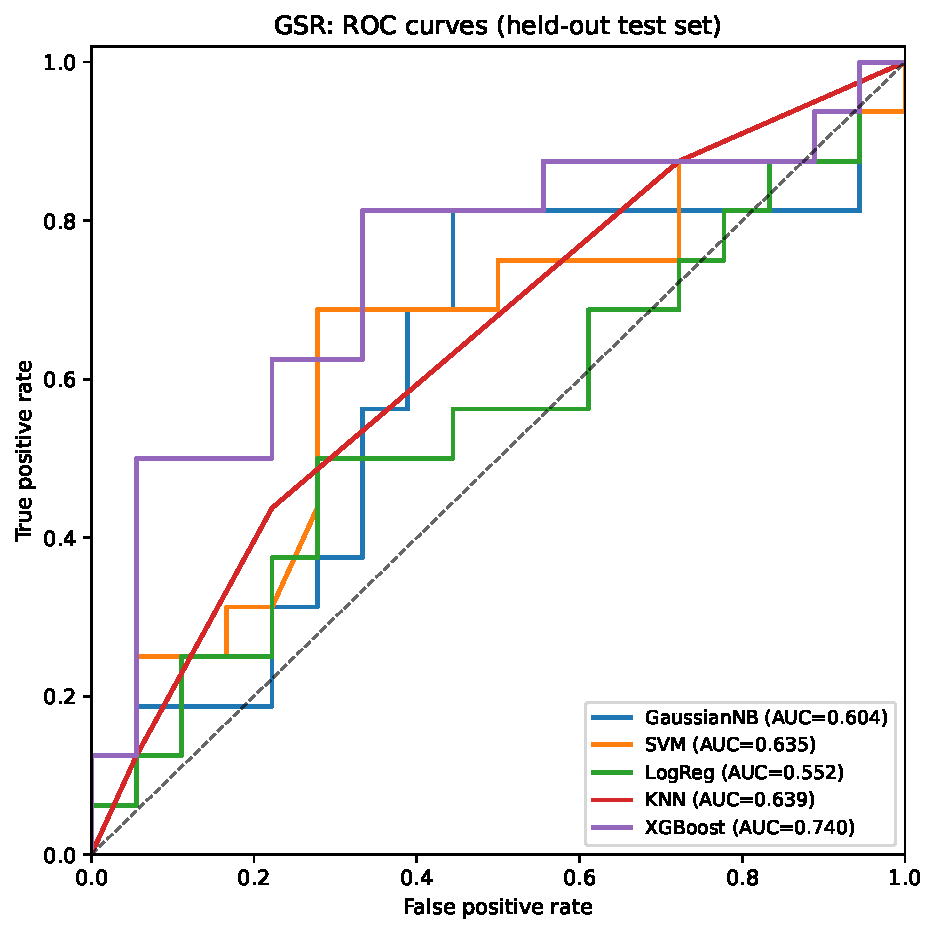
\includegraphics[width=0.6\linewidth]{../../Images/GSR_roc.pdf}
%DIFDELCMD <   %%%
%DIFDELCMD < \caption{%
{%DIFAUXCMD
\DIFdelFL{Receiver operating characteristic (ROC) curves for ASD versus TD classification on the
  held-out test set, GSR pipeline, after ComBat harmonization. The diagonal grey line indicates
  chance. Curves lie near the diagonal (best cross-validated accuracy $\approx 0.59$), indicating
  near-chance discrimination from the harmonized coevolutionary and connectivity features.}}
  %DIFAUXCMD
%DIFDELCMD < \label{fig:ml_confusion_roc}
%DIFDELCMD < \end{figure}
%DIFDELCMD < %%%
\DIFdelend \DIFaddbegin \paperfigure{Fig10}{Balanced accuracy and conditional uncertainty}{Each classifier has complete out-of-fold predictions for all 140 participants. Symbols distinguish GSR and no-GSR; colors identify model families. Intervals are 95 percentiles from 1,000 site-bootstrap replicates conditional on the saved predictions and omit full retraining and upstream QC uncertainty. Every interval includes .5. No final model is selected from these outer results.}{fig:classifiers}
\DIFaddend 


\DIFdelbegin %DIFDELCMD < \begin{figure}[H]
%DIFDELCMD <   \centering
%DIFDELCMD <   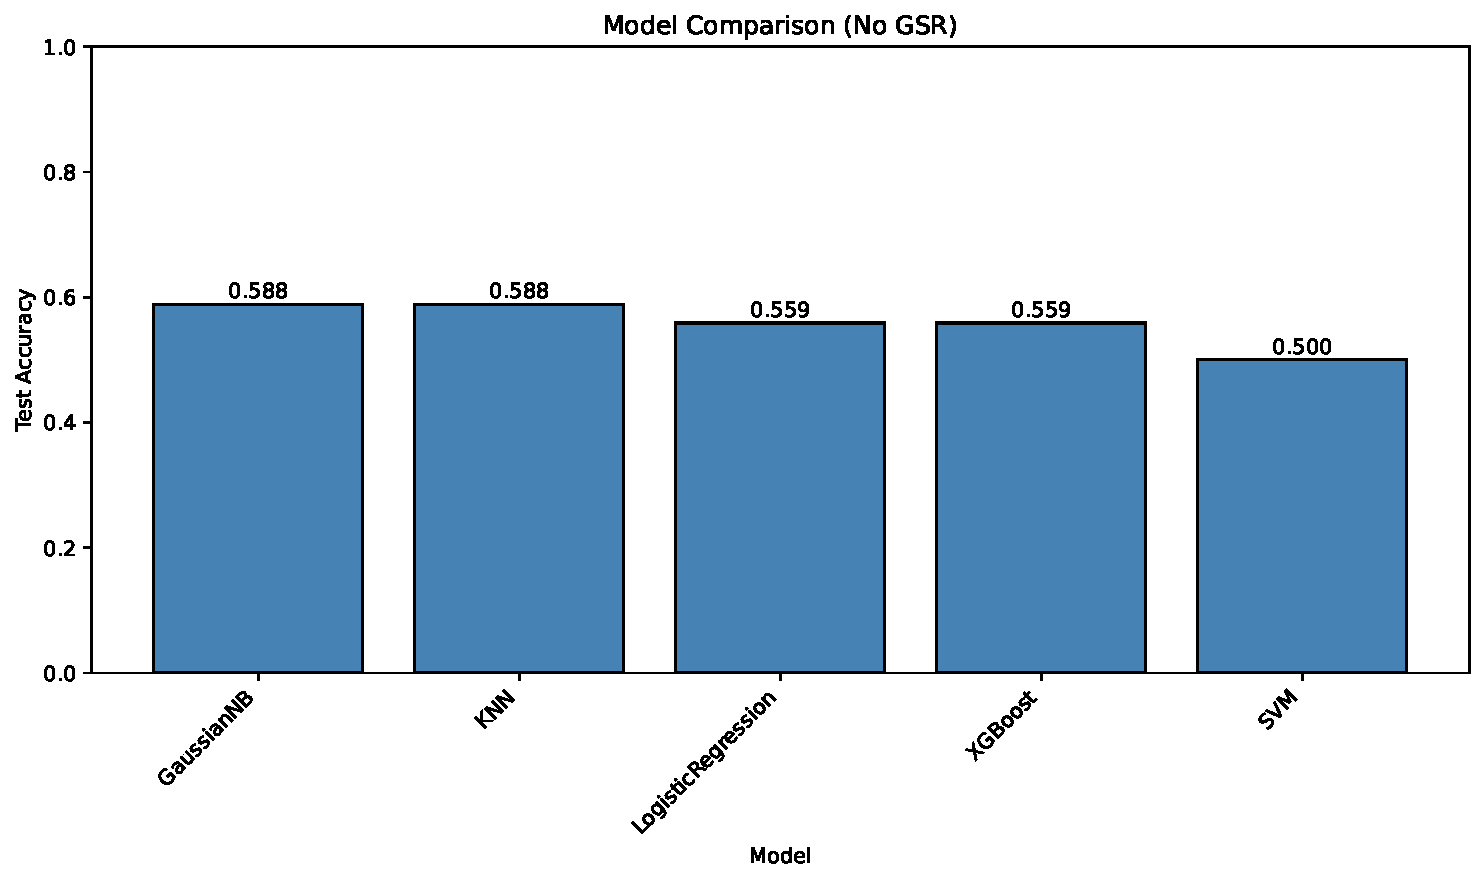
\includegraphics[width=0.7\linewidth]{../../Images/model_comparison_GSR.pdf}
%DIFDELCMD <   %%%
%DIFDELCMD < \caption{%
{%DIFAUXCMD
\DIFdelFL{Summary of classifier performance (GSR pipeline, harmonized features). Cross-validated
  accuracy was at or near chance ($0.56$--$0.59$) across all five models; held-out test accuracies
  varied between $50\%$ and $65\%$ on the small test set ($n = 34$) and do not indicate reliable
  discrimination.}}
  %DIFAUXCMD
%DIFDELCMD < \label{fig:ml_barplot}
%DIFDELCMD < \end{figure}
%DIFDELCMD < %%%
\DIFdelend \DIFaddbegin \begin{table}[H]
\centering\small
\caption{\textbf{Complete site-held-out classification results.}}\label{tab:classification}
\begin{tabular}{llrrlrr}
\toprule
Pipeline & Model & Accuracy & BA & BA 95\% CI & F1 & AUC \\
\midrule
GSR & GNB & 0.500 & 0.498 & 0.428, 0.583 & 0.435 & 0.513 \\
GSR & KNN & 0.521 & 0.518 & 0.455, 0.581 & 0.385 & 0.505 \\
GSR & LR & 0.536 & 0.534 & 0.469, 0.613 & 0.488 & 0.535 \\
GSR & SVM & 0.557 & 0.558 & 0.464, 0.653 & 0.569 & 0.573 \\
GSR & XGB & 0.457 & 0.457 & 0.390, 0.531 & 0.441 & 0.485 \\
noGSR & GNB & 0.514 & 0.515 & 0.401, 0.633 & 0.528 & 0.499 \\
noGSR & KNN & 0.543 & 0.542 & 0.470, 0.627 & 0.522 & 0.518 \\
noGSR & LR & 0.486 & 0.485 & 0.428, 0.559 & 0.463 & 0.451 \\
noGSR & SVM & 0.486 & 0.485 & 0.385, 0.591 & 0.471 & 0.512 \\
noGSR & XGB & 0.507 & 0.507 & 0.439, 0.615 & 0.481 & 0.536 \\
\bottomrule
\end{tabular}
\begin{flushleft}\footnotesize
Every row uses 140 OOF predictions (69 ASD/71 controls). BA: balanced accuracy; F1 treats ASD as positive. Intervals bootstrap sites conditional on fixed predictions and omit part of training uncertainty. LR: logistic regression; SVM: radial-basis support vector machine; GNB: Gaussian naive Bayes; KNN: k-nearest neighbors; XGB: XGBoost. All models are reported without an outer-test winner.
\end{flushleft}
\end{table}

\DIFaddend 

\DIFdelbegin \paragraph*{\DIFdel{Feature selection and importance-ranked feature set.}}
%DIFAUXCMD
\DIFdel{To reduce dimensionality and focus the classifiers on the most informative descriptors, we performed
a single feature selection step }\emph{\DIFdel{before}} %DIFAUXCMD
\DIFdel{model-specific training and tuning. This feature
selection step used a Random Forest classifier , applied only to the training data, to rank features
by mean decrease in impurity. Starting from the full set of 90 graph-based features (whole-brain
coevolutionary metrics, intra-network energies, }\DIFdelend %DIF >  ML_SELECTION_RESULTS_BEGIN
\DIFaddbegin \paragraph*{\DIFadd{Feature-selection audit and exploratory extension.}}
\DIFadd{Feature selection was already nested in the five-model analysis above. Reconstructing
all 50 outer-training fits reproduces every saved prediction: ANOVA retained 22
features in 11 fits, 44 in 17, and all 88 in 22. We subsequently compared broader
selection methods in a separate exploratory analysis, retaining the same known
outer site folds rather than treating them as a fresh independent test.
Training-fold near-exact redundancy pruning left 59 distinct columns, }\DIFaddend and \DIFdelbegin \DIFdel{inter-network connectivity and energy terms), we fitted a random forest classifier on the training set only and extracted the importance for each
feature . Features were then ranked by importance, and we retained the top 25\% (23 features) as
the final input feature set for all subsequent classifiers}\DIFdelend \DIFaddbegin \DIFadd{inner
CV chose all 59 in seven fits, ANOVA top-K in 16, mutual-information top-K in 17,
and L1-ranked top-K in ten. Additional selection retained 5, 10 or 20 features}\DIFaddend .

\DIFdelbegin \DIFdel{The full importance ranking from the harmonized GSR pipeline is shown in
Fig~\ref{fig:ml_selected_features}. Because classification accuracy is at or near chance after
harmonization, this ranking should be interpreted cautiously: with no reliable group-discriminative
signal, the random forest is ranking features that contribute little above chance,
}\DIFdelend \DIFaddbegin \DIFadd{Four of the ten model/pipeline point estimates increased and six decreased
(Table~\ref{tab:selection}). No-GSR logistic regression changed from .485 to
.544, no-GSR SVM from .485 to .536, }\DIFaddend and \DIFdelbegin \DIFdel{the ordering
is not stable evidence of diagnostic relevance. The highest-ranked descriptors are predominantly
inter-network average-connectivity terms (involving SomatoMotor, attention, frontoparietal,
}\DIFdelend \DIFaddbegin \DIFadd{no-GSR KNN from .542 to .557. GSR XGBoost
changed from .457 to .492. Every paired conditional interval for change includes
zero, }\DIFaddend and \DIFdelbegin \DIFdel{default-mode systems) together with whole-brain motif proportions, broadly echoing the directions of
the (non-significant) univariate trends.
}%DIFDELCMD < 

%DIFDELCMD < \begin{figure}[H]
%DIFDELCMD < \centering
%DIFDELCMD < 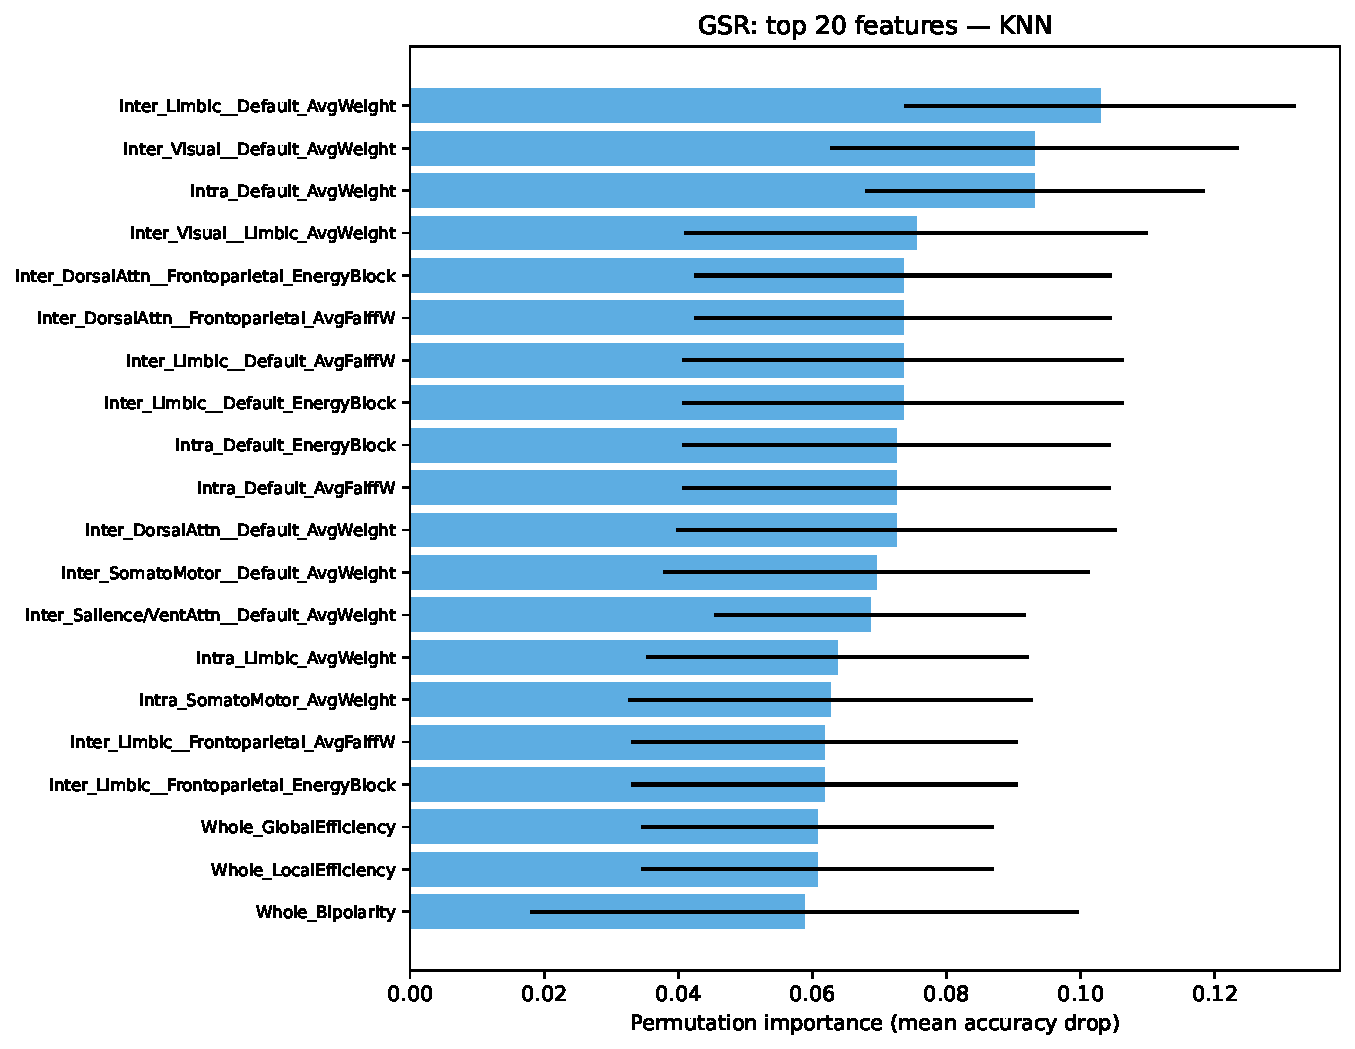
\includegraphics[width=0.8\linewidth]{../../Images/GSR_feature_importance.pdf}
%DIFDELCMD < %%%
%DIFDELCMD < \caption{%
{%DIFAUXCMD
\DIFdelFL{Random-forest feature-importance ranking for ASD--TD classification (GSR pipeline,
harmonized features). Because the classifiers performed at or near chance
(Table~\ref{tab:ml_summary_full}), this ranking is exploratory and does not establish
diagnostic relevance of any feature.}}
%DIFAUXCMD
%DIFDELCMD < \label{fig:ml_selected_features}
%DIFDELCMD < \end{figure}
%DIFDELCMD < 

%DIFDELCMD < %%%
\DIFdel{Overall, the classificationanalysis reinforces the main univariate finding: after site
harmonization, the coevolutionary and signed-connectivity features do not reliably distinguish ASD
from TD in this sample.
}\DIFdelend \DIFaddbegin \DIFadd{all follow-up balanced-accuracy intervals include .5. }\DIFaddend The \DIFdelbegin \DIFdel{feature-importance ranking is provided for completeness and as a
hypothesis-generating description rather than as evidence of a diagnostic signature.
}%DIFDELCMD < 

%DIFDELCMD < %%%
\subsection*{\DIFdel{Sensitivity analysis: results without global signal regression}}
%DIFAUXCMD
%DIFDELCMD < 

%DIFDELCMD < %%%
\DIFdel{Because GSR can introduce artifactual negative correlations }%DIFDELCMD < \cite{Murphy2009,Fox2009,Chang2009}
%DIFDELCMD < %%%
\DIFdel{and the sign of functional links is a key parameter in the coevolutionary framework, we repeated
all primary analyses on data preprocessed without GSR}\DIFdelend \DIFaddbegin \DIFadd{follow-up
therefore does not establish a reliable performance gain or justify selecting a
new final classifier from the outer results. Full ROC, confusion, performance
and selected-feature frequency heatmaps are in S1 Appendix; all
feature names, inner candidates, and test predictions are in S2}\DIFaddend .
\DIFdelbegin \DIFdel{This alternative pipeline used CompCor-based
denoising (anatomical noise components from white matter and CSF }%DIFDELCMD < \cite{Behzadi2007}%%%
\DIFdel{), retaining all
other preprocessing steps (motion regression,
bandpass filtering, ComBat harmonization, parcellation)
identically to the primary analysis. The no-GSR sensitivity results reported here therefore
correspond to a CompCor-only denoising strategy.
After identical quality control and Tukey IQR-based
outlier removal, the no-GSR sample comprised 78 ASD and 87 TD participants.
}\DIFdelend 

\DIFdelbegin \paragraph*{\DIFdel{Whole-brain metrics.}}
%DIFAUXCMD
\DIFdel{As in the GSR-based analysis , global coevolutionary energy did not differ significantly
between groups in the
no-GSR pipeline (ASD: $-285.4 \pm 146.1$; TD: $-308.3 \pm 155.7$;
Mann--Whitney $U$, $p = 0.305$). The proportions of agreement, disagreement, imbalanced-same, and imbalanced-opposite links also did not reach significance after FDR correction
(all $p_{\mathrm{FDR}} > 0.23$; Table~\ref{tab:noGSR_whole}). Whole-brain bipolarity showed the
strongest nominal whole-brain difference (ASD: $0.591 \pm 0.043$; TD: $0.577 \pm 0.045$;
Mann--Whitney $U$, uncorrected $p = 0.026$), with the
ASD group exhibiting slightly higher bipolarity, in the direction of a stronger two-block organization of the signed network when negative
correlations are not induced by GSR (Eq.~\ref{eq:bipolarity}). After FDR correction across the eight
whole-brain features, however, this effect was not significant ($p_{\mathrm{FDR}} = 0.21$).
Because
bipolarity does not differ between groups under GSR ($p = 0.53$), even this nominal trend is
pipeline-dependent and
should be regarded as hypothesis-generating rather than confirmatory.
}\DIFdelend \DIFaddbegin \begin{table}[H]
\centering\small
\caption{\textbf{Exploratory feature-selection comparison on the same known outer folds.}}\label{tab:selection}
\begin{tabular}{llrrrl}
\toprule
Pipeline & Model & Baseline BA & Follow-up BA & Change & Change 95\% CI \\
\midrule
GSR & GNB & 0.498 & 0.491 & -0.008 & -0.092, 0.074 \\
GSR & KNN & 0.518 & 0.442 & -0.076 & -0.193, 0.024 \\
GSR & LR & 0.534 & 0.521 & -0.013 & -0.107, 0.036 \\
GSR & SVM & 0.558 & 0.534 & -0.023 & -0.097, 0.068 \\
GSR & XGB & 0.457 & 0.492 & 0.036 & -0.031, 0.103 \\
noGSR & GNB & 0.515 & 0.493 & -0.022 & -0.086, 0.038 \\
noGSR & KNN & 0.542 & 0.557 & 0.014 & -0.098, 0.108 \\
noGSR & LR & 0.485 & 0.544 & 0.059 & -0.015, 0.109 \\
noGSR & SVM & 0.485 & 0.536 & 0.051 & -0.038, 0.148 \\
noGSR & XGB & 0.507 & 0.500 & -0.006 & -0.149, 0.078 \\
\bottomrule
\end{tabular}
\begin{flushleft}\footnotesize
Paired change intervals resample sites conditional on fixed OOF predictions. The follow-up was specified after baseline results had been examined and is not independent confirmation of improvement. Representation and XGBoost search grids also differ. All ten estimates are shown; no classifier is selected by outer performance.
\end{flushleft}
\end{table}

%DIF >  ML_SELECTION_RESULTS_END
\DIFaddend 

\DIFdelbegin \DIFdel{Global and local graph efficiency, which were computed within the }\DIFdelend \DIFaddbegin \subsection*{\DIFadd{Sensitivity analysis: results without global signal regression}}
\DIFadd{The original }\DIFaddend no-GSR \DIFdelbegin \DIFdel{pipeline, did not differ
significantly between ASD and TD groups (both $p = 0.25$).
However, graph efficiency showed a significant negative correlation with $H$ within the ASD group (global efficiency: $r = -0.33$,
$p = 0.003$, FDR $p = 0.005$; local efficiency: $r = -0.33$, FDR $p = 0.005$), indicating that more
coevolutionarily stable ASD networks tend to be less globally and locally efficient. This
relationship was weaker and not significant in the TD group ($r = -0.17$, $p = 0.12$),
and in the
GSR pipeline it was a non-significant trend within ASD ($r = -0.20$, $p = 0.075$), so it too is
pipeline-dependent. This analysis, together with the relationship between $H$ and
other network metrics, is detailed below (see ``Relationship between the Hamiltonian and other
network metrics''). }%DIFDELCMD < 

%DIFDELCMD < \begin{figure}[H]
%DIFDELCMD <  \centering
%DIFDELCMD <  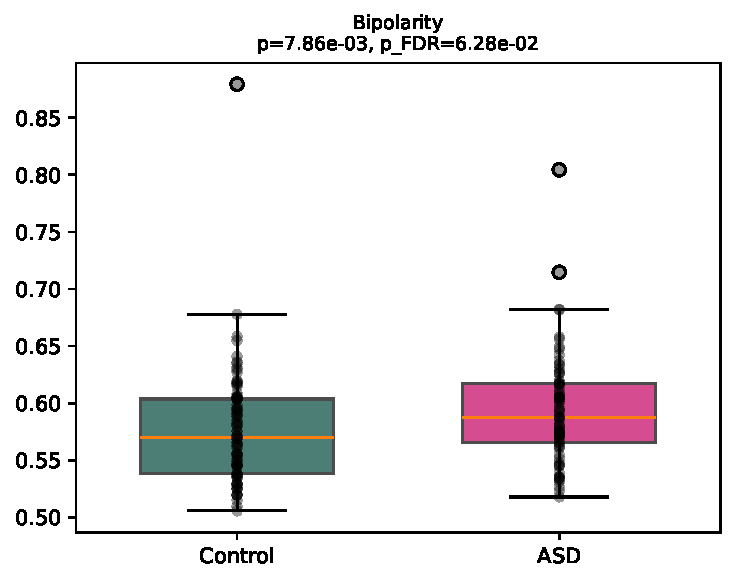
\includegraphics[width=0.55\linewidth]{../../Images/Whole_significant_noGSR.pdf}
%DIFDELCMD <  %%%
%DIFDELCMD < \caption{%
{%DIFAUXCMD
\DIFdelFL{Whole-brain bipolarity in the no-GSR sensitivity analysis (CompCor preprocessing,
 harmonized; $n = 78$ ASD, $87$ TD). Bipolarity showed the strongest whole-brain nominal group
 difference (uncorrected $p = 0.026$), with ASD exhibiting slightly higher bipolarity (stronger
 two-block organization) than TD. After FDR correction across the eight whole-brain features, this
 effect was not significant ($p_{\mathrm{FDR}} = 0.21$). In the GSR pipeline, bipolarity did not
 differ between groups ($p = 0.53$), so even this nominal trend is pipeline-dependent.}}
 %DIFAUXCMD
%DIFDELCMD < \label{fig:noGSR_whole}
%DIFDELCMD < \end{figure}
%DIFDELCMD < 

%DIFDELCMD < %%%
\paragraph*{\DIFdel{Relationship between the Hamiltonian and other network metrics.}}
%DIFAUXCMD
\DIFdel{Because graph efficiency was incorporated into the whole-brain feature family of the }\DIFdelend \DIFaddbegin \DIFadd{sensitivity remains explicit at each scale: global quantities,
within-network and between-network group contrasts, H--metric associations,
clinical analyses, PLS, and classification. Primary participant and node sets are
identical across pipelines. GSR/}\DIFaddend no-GSR \DIFdelbegin \DIFdel{pipeline, the relationship between the Hamiltonian and other network measures was characterized under this
pipeline, where it provides an independent validation of the coevolutionary framework.
We computed
correlations between $H(G)$ and all other network features (both intra-network and inter-network)
within each group separately, and separately related the global Hamiltonian to global graph
efficiency and the local efficiency measure, which are standard indices of network integration and
segregation }%DIFDELCMD < \cite{Latora2001,Fornito2016}%%%
\DIFdel{. }\DIFdelend \DIFaddbegin \DIFadd{Hamiltonian diagnosis estimates are both
imprecise; ComBat and pooled trimming do not yield a corrected group difference.
Larger-node sensitivity designs change participants as well as nodes.
The original spectral-bipolarity descriptor is now reported separately as an
exploratory raw adjusted comparison: coefficients are .00040 with GSR and .01055
without GSR, with Holm $p=.916$ for both. It remains outside the frozen feature
families and does not alter the common clinical/predictive schema.
}\DIFaddend 

\DIFdelbegin \DIFdel{Within the ASD group, $H$ was significantly correlated with multiple inter-network AvgFalffW and
EnergyBlock features (FDR $p < 10^{-7}$ for the strongest associations), which is expected given
the mathematical relationship between these measures and the Hamiltonian.
More informative from an
independent-validation standpoint are the correlations with AvgWeight features, which measure pure
functional connectivity strength without any fALFF-weighting and are therefore not mathematically
derived from $H$.
Within ASD, more negative $H$ was significantly associated with lower mean FC
across multiple networks including SomatoMotor--Default, intra-SomatoMotor, Visual--SomatoMotor, }\DIFdelend %DIF >  CLASSIFICATION_CONTINUITY_BEGIN
\DIFaddbegin \DIFadd{All five original algorithm types have complete OOF predictions in both pipelines,
using the same revision participants, features, folds and scoring.
Matching the algorithm types does not restore identical original inputs or validation:
site-held-out evaluation replaces the original random train/test procedure.
%DIF >  CLASSIFICATION_CONTINUITY_END
}


\section*{\DIFadd{Discussion}}\linelabel{lin:discussion}
\DIFadd{The revised analysis does not detect a corrected diagnosis effect in the
coverage-defined adult male sample. Raw covariate-adjusted models, explicit
ComBat sensitivities, pooled trimming, and mixed-diagnosis-site restriction are
consistent in this limited sense. The separate male-control null comparison supports alignment relative to the
specified state randomizations, while the diagnosis comparison asks a different
question. Alignment in controls can coexist with no detectable diagnosis contrast.
Their uncertainty remains substantial, }\DIFaddend and
\DIFdelbegin \DIFdel{SomatoMotor--DorsalAttn (all FDR $p \approx 0.009$, $r \approx -0.31$). Within
the TD group, the corresponding AvgWeight--$H$ correlations were weaker. This
pattern
suggests that in ASD, coevolutionary stability is not simply a reflection of higher mean connectivity;
rather,
it arises from the signed configuration of links relative to nodal states,
independently of
overall connectivity magnitude.
}\DIFdelend \DIFaddbegin \DIFadd{inconclusive equivalence tests preclude a universal adult-null interpretation.
The multisite generalization difficulties reported for FC more broadly
}\cite{King2019revision} \DIFadd{reinforce the need for larger independent tests.
}\DIFaddend 

\DIFdelbegin \DIFdel{Comparing the global Hamiltonian with the global integration measure, more negative }\DIFdelend \DIFaddbegin \DIFadd{This result concerns a relative fALFF--FC alignment statistic. Median states do
not distinguish globally elevated from globally reduced fALFF distributions,
and identical values can receive different labels across participants. It is
therefore inappropriate to equate $+1$ with high neuronal firing or to interpret
}\DIFaddend $H$ \DIFdelbegin \DIFdel{(greater
coevolutionary stability) was significantly associated with lower global efficiency within the ASD
group ($r = -0.33$, $p = 0.003$, FDR $p = 0.005$); the corresponding local-scale comparison, between
$H$ and local efficiency, showed an effect of the same magnitude and direction ($r = -0.33$,
FDR $p = 0.005$; Fig~\ref{fig:hamil_correlates}). Within the TD group this relationship was
weaker and not significant ($r = -0.17$, $p = 0.12$). These results show
that in ASD, greater alignment between nodal activity states and signed connectivity comes at a measurable cost to network integration efficiency. The }\DIFdelend \DIFaddbegin \DIFadd{as metabolic cost. Construction also links the statistic to global weights;
the original descriptive H--metric question still produces corrected
within-group associations, whereas the controlled efficiency analyses do not
retain the submitted }\DIFaddend ASD-specific \DIFdelbegin \DIFdel{strengthening of this
relationship may reflect a }\DIFdelend trade-off \DIFdelbegin \DIFdel{between energetic stability and flexible network communication
that is more pronounced in the autistic brain. We caution that this analysis is observational and
cross-sectional; whether the stability--efficiency trade-off reflects a causal mechanism remains an
open question .
}%DIFDELCMD < 

%DIFDELCMD < \begin{figure}[H]
%DIFDELCMD <  \centering
%DIFDELCMD <  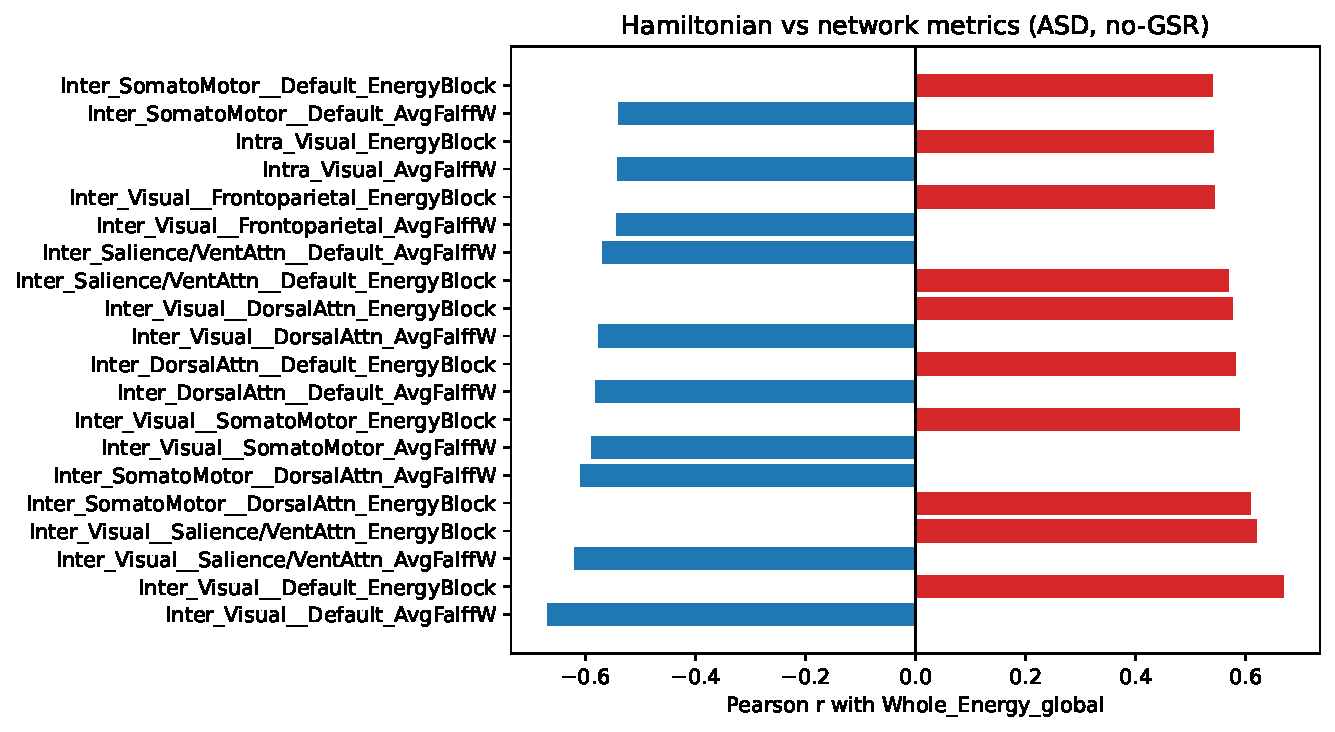
\includegraphics[width=0.85\linewidth]{../../Images/Hamiltonian_correlates_ASD_noGSR.pdf}
%DIFDELCMD <  %%%
%DIFDELCMD < \caption{%
{%DIFAUXCMD
\DIFdelFL{Top 20 network metrics most strongly correlated with whole-brain coevolutionary energy
 ($H$) within the ASD group (no-GSR pipeline). Red bars indicate positive correlations (EnergyBlock
 features, which are negatively signed relatives of AvgFalffW and share the same information);
 blue bars indicate negative correlations. Note that AvgWeight features (pure FC magnitude, no
 fALFF-weighting) are also present among the strongest correlates, confirming that the Hamiltonian
 captures information beyond average connectivity. The two blue bars at the lower end of the ranking
 correspond to global and local graph efficiency; the global Hamiltonian is most directly compared
 with global efficiency, and the local efficiency measure provides the corresponding local-scale
 comparison. Their negative correlation with $H$ within ASD (FDR $p = 0.006$) indicates that more
 coevolutionarily stable networks tend to be less efficiently integrated.}}
 %DIFAUXCMD
%DIFDELCMD < \label{fig:hamil_correlates}
%DIFDELCMD < \end{figure}
%DIFDELCMD < 

%DIFDELCMD < %%%
\paragraph*{\DIFdel{Intra-network metrics.}}
%DIFAUXCMD
\DIFdel{At the intra-network level, only Dorsal Attention network average connectivity (AvgWeight) showed
an uncorrected group difference (ASD: $0.274 \pm 0.118$; TD: $0.310 \pm 0.121$; $p = 0.039$), with lower connectivity in ASD, but this did not survive FDR correction ($p_{\mathrm{FDR}} = 0.32$;
Fig~\ref{fig:noGSR_intra}). No other intra-network metrics reached uncorrected significance.
}\DIFdelend \DIFaddbegin \DIFadd{interpretation. An association between two summaries of the same FC matrix would
not independently validate a biological mechanism even if statistically detected.
}\DIFaddend 

\DIFdelbegin %DIFDELCMD < \begin{figure}[H]
%DIFDELCMD <  \centering
%DIFDELCMD <  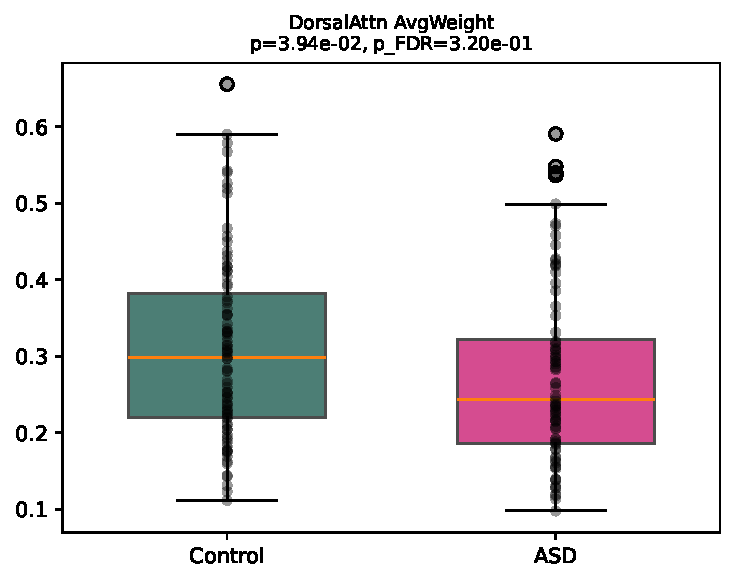
\includegraphics[width=0.55\linewidth]{../../Images/Intra_significant_noGSR.pdf}
%DIFDELCMD <  %%%
%DIFDELCMD < \caption{%
{%DIFAUXCMD
\DIFdelFL{Intra-network metric showing the largest uncorrected group difference in the no-GSR
 analysis: Dorsal Attention network average connectivity ($p = 0.039$, $p_{\mathrm{FDR}} = 0.32$).
 This did not survive FDR correction.}}
 %DIFAUXCMD
%DIFDELCMD < \label{fig:noGSR_intra}
%DIFDELCMD < \end{figure}
%DIFDELCMD < %%%
\DIFdelend \DIFaddbegin \DIFadd{The result differs in scope from our earlier developmental triadic-balance work
}\cite{Moradimanesh2021} \DIFadd{and from temporal energy-landscape studies
}\cite{Watanabe2017revision}\DIFadd{. Different ages, state definitions, parcellations, and
statistics can test different hypotheses. Regional adult fALFF findings
}\cite{Itahashi2015revision} \DIFadd{can coexist with a null global rank-based summary.
We cannot infer developmental normalization or disagreement with dynamic-state
findings from this adult cross-sectional analysis.
}\DIFaddend 

\DIFdelbegin \paragraph*{\DIFdel{Inter-network metrics.}}
%DIFAUXCMD
\DIFdel{No inter-network metrics reached significance after FDR correction in the no-GSR analysis (all
$p_{\mathrm{FDR}} > 0.35$). Several network pairs involving the dorsal attention and somatomotor
networks showed nominally significant trends in average connectivity (SomatoMotor--DorsalAttn:
$p = 0.050$; DorsalAttn--Limbic: $p = 0.058$; DorsalAttn--Default: $p = 0.059$;
Fig~\ref{fig:noGSR_inter}), consistent with }\DIFdelend \DIFaddbegin \subsection*{\DIFadd{Regional organization and mathematical dependence}}
\DIFadd{The lack of a corrected global diagnosis effect could, in principle, conceal
opposing regional changes. The within- and between-network analyses explicitly
address that possibility: all available cortical blocks are tested rather than
choosing a few networks after inspecting their nominal probabilities. Their
uncorrected contrasts do not survive the specified family corrections. This
limits the present evidence for spatially localized group effects; it does not
show that each cortical system is equivalent between groups. In particular,
}\DIFaddend the \DIFdelbegin \DIFdel{general pattern of lower connectivity in ASD
observed in the GSR analysis}\DIFdelend \DIFaddbegin \DIFadd{single retained limbic parcel makes within-limbic comparisons unavailable,
so a limbic null conclusion would be unsupported}\DIFaddend .

\DIFdelbegin %DIFDELCMD < \begin{figure}[H]
%DIFDELCMD <  \centering
%DIFDELCMD <  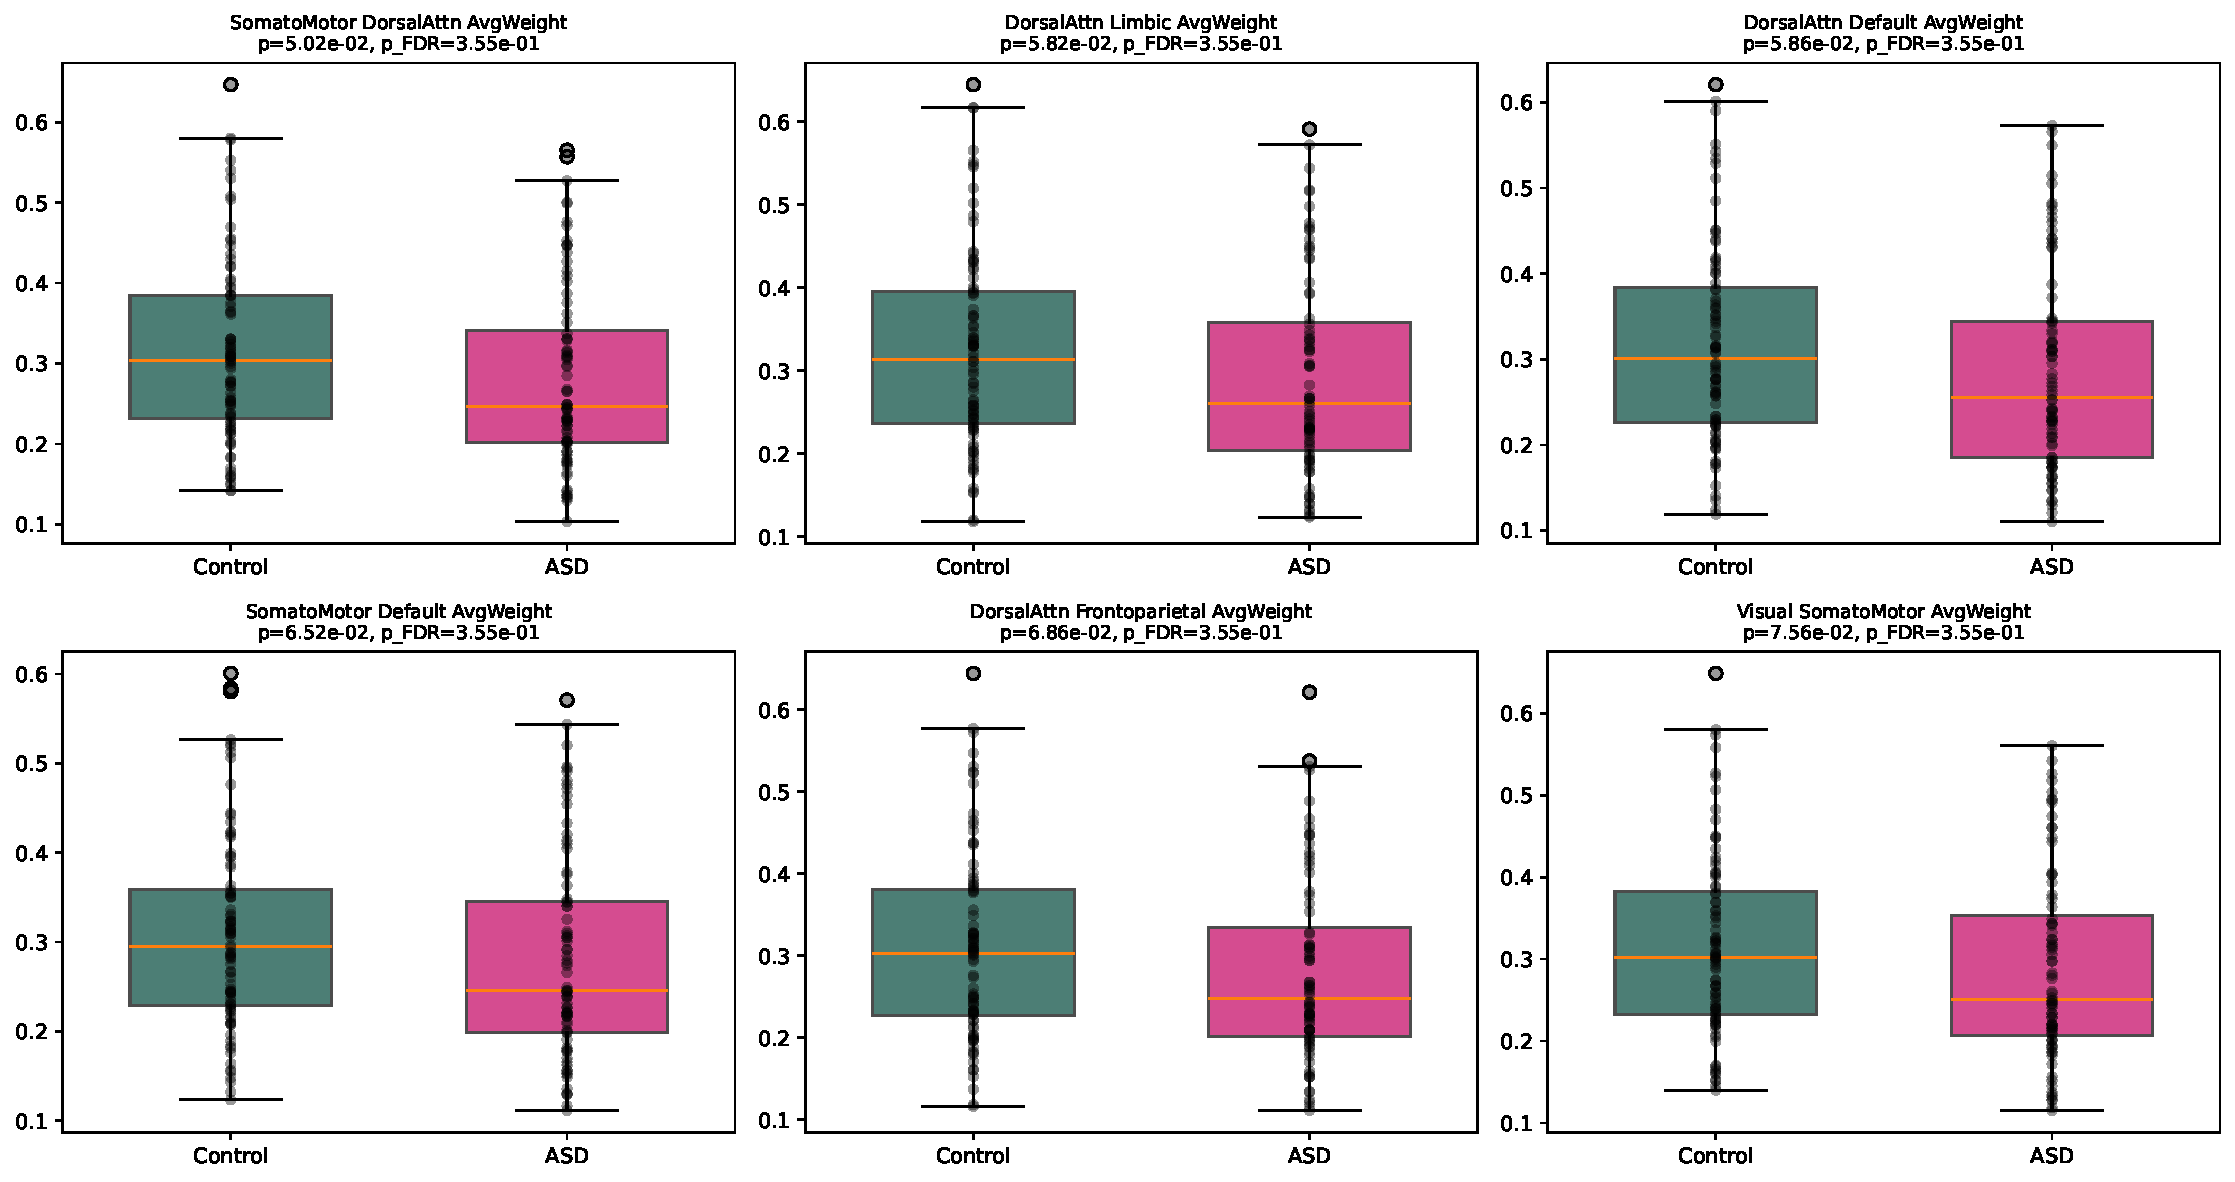
\includegraphics[width=0.95\linewidth]{../../Images/Inter_significant_noGSR.pdf}
%DIFDELCMD <  %%%
%DIFDELCMD < \caption{%
{%DIFAUXCMD
\DIFdelFL{Inter-network average connectivity metrics with the smallest $p$-values in the no-GSR
 sensitivity analysis. None survived FDR correction (all $p_{\mathrm{FDR}} > 0.35$). Effects are
 generally weaker and fewer than in the GSR-based analysis.}}
 %DIFAUXCMD
%DIFDELCMD < \label{fig:noGSR_inter}
%DIFDELCMD < \end{figure}
%DIFDELCMD < %%%
\DIFdelend \DIFaddbegin \DIFadd{The descriptive H--metric analysis has a different outcome and purpose. Several
within-group associations survive its stated correction, preserving an important
part of the original study. Their interpretation depends on construction.
Block energy is a component of the global sum, and multiplying mean
state-weighted FC by a fixed negative edge count reproduces that block's energy.
Consequently, significant correlations between these measures can describe how
a global statistic is distributed across networks without constituting
independent replications or identifying a mechanism. Nor does a significant
association in ASD and a nonsignificant association in controls establish that
the two associations differ. The adjusted interaction tests directly address
that stronger question for efficiency and provide no corrected support for it.
}\DIFaddend 

\DIFdelbegin \paragraph*{\DIFdel{Behavioral correlations under CompCor preprocessing.}}
%DIFAUXCMD
\DIFdel{Behavioral correlations were also computed under the no-GSR (CompCor) pipeline, providing a direct
comparison with the primary GSR results. Using
the same procedure (Pearson and Spearman $r$, FDR correction across 460 tests: 92 features
$\times$ 5 clinical scores
with sufficient data), no feature--clinical score association survived
FDR correction ($q < 0.05$). At the nominally significant threshold ($p < 0.05$), 31 pairs were
detected across all five scores---again close to the chance expectation.
}\DIFdelend The \DIFdelbegin \DIFdel{strongest associations
involved inter-network SomatoMotor--Default fALFF-aligned connectivity with ADOS Total ($r = -0.34$,
$p = 0.008$; $n = 60$), intra-network Limbic energy with ADOS Communication ($r = -0.37$,
$p = 0.009$; $n = 50$), and inter-network DorsalAttn--Limbic fALFF-aligned connectivity with ADI-R
Social ($r = +0.45$, $p = 0.008$; $n = 33$). The Hamiltonian did not show a significant within-ASD
correlation with ADOS Total in the no-GSR pipeline ($r = +0.05$, $p = 0.71$), consistent with the GSR result ($r = -0.10$}\DIFdelend \DIFaddbegin \DIFadd{empirical-null results also depend on what is held fixed. Both null schemes
preserve every FC weight, the observed number of nodal labels, and the graph's
topology. They test reassignment of regional states, not whether the empirical
FC network is unusually organized compared with rewired graphs. Constraining
permutations by network and hemisphere yields less extreme alignment scores}\DIFaddend ,
\DIFdelbegin \DIFdel{$p = 0.47$): in neither pipeline, after harmonization, is whole-brain
energy associated with symptom severity.
}\DIFdelend \DIFaddbegin \DIFadd{consistent with some organization already being retained by the null. Remaining
alignment can reflect finer spatial structure, biological organization, or
shared measurement characteristics. A null model defines the comparison rather
than furnishing a universal test of randomness }\cite{VasaMisic2022revision}\DIFadd{.
}\DIFaddend 

\DIFdelbegin \paragraph*{\DIFdel{Machine learning classification.}}
%DIFAUXCMD
\DIFdel{Classification under the no-GSR pipeline was also at or near chance after harmonization. The best }\DIFdelend \DIFaddbegin \subsection*{\DIFadd{Clinical relevance and predictive evaluation}}
\DIFadd{Clinical correlation, latent covariance, and }\DIFaddend held-out \DIFdelbegin \DIFdel{test accuracy was $0.59$ (Gaussian Naive Bayes), with cross-validated accuracies of $0.46$--$0.57$ across the five classifiers (Table~\ref{tab:noGSR_ml}; Fig~\ref{fig:noGSR_ml}). As in the GSR pipeline, this is consistent with the absence of FDR-significant univariate group
differences: neither preprocessing strategy yields features that reliably discriminate ASD from TD
after site harmonization. }%DIFDELCMD < 

%DIFDELCMD < \begin{figure}[H]
%DIFDELCMD <   \centering
%DIFDELCMD <   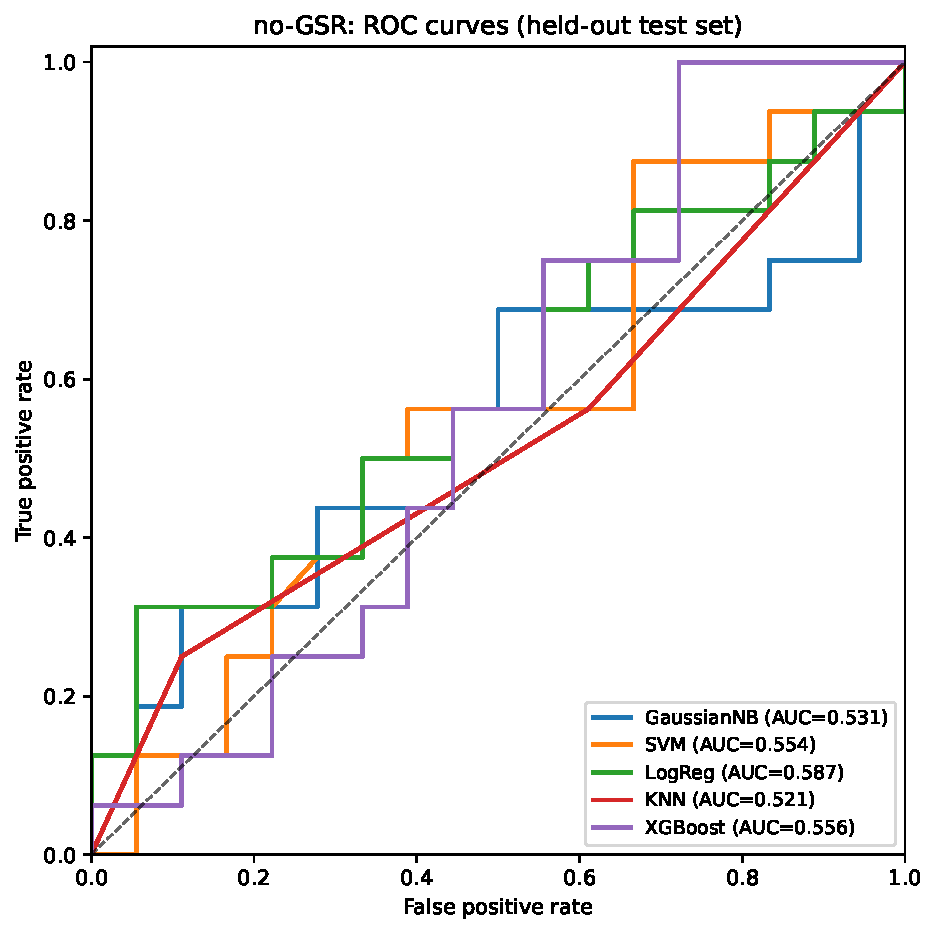
\includegraphics[width=0.6\linewidth]{../../Images/no-GSR_roc.pdf}
%DIFDELCMD <   %%%
%DIFDELCMD < \caption{%
{%DIFAUXCMD
\DIFdelFL{ROC curves for ASD versus TD classification in the no-GSR sensitivity analysis (CompCor
  preprocessing, harmonized features). Curves lie near the chance diagonal; the best held-out test
  accuracy was $0.59$ (Gaussian Naive Bayes), again indicating near-chance discrimination, as in the
  GSR pipeline (Fig~\ref{fig:ml_confusion_roc}).}}
  %DIFAUXCMD
%DIFDELCMD < \label{fig:noGSR_ml}
%DIFDELCMD < \end{figure}
%DIFDELCMD < 

%DIFDELCMD < %%%
\paragraph*{\DIFdel{Summary of the sensitivity analysis.}}
%DIFAUXCMD
\DIFdel{Table~\ref{tab:GSR_comparison} provides a side-by-side comparison of key results across the two
preprocessing pipelines after harmonization, together with the effect of harmonization itself.
The
two pipelines agree on the central outcome: after correct harmonization and FDR correction, no
whole-brain, intra-network, or inter-network feature differs significantly between groups under
either GSR or CompCor.
The strongest nominal whole-brain trend differs by pipeline (more negative
energy under GSR, $p = 0.048$; slightly higher bipolarity under CompCor, $p = 0.026$), but neither
survives correction, and bipolarity does not
differ at all under GSR. The within-ASD association
between $H$ and graph efficiency is the one effect that reaches FDR significance, and only in the
no-GSR pipeline. Classification on the harmonized features was at or near chance in both pipelines
(Tables~\ref{tab:ml_summary_full} and ~\ref{tab:noGSR_ml}).
These patterns are discussed further below,
including the decisive
effect of harmonization itself.
}%DIFDELCMD < 

%DIFDELCMD < %%%
\section*{\DIFdel{Discussion}}
%DIFAUXCMD
%DIFDELCMD < 

%DIFDELCMD < %%%
\DIFdel{In this study we used a coevolutionary balance framework to characterize how resting-state
functional networks are organized in adult males with autism spectrum disorder.
By combining
binarized regional activity (fractional amplitude of low-frequency fluctuations, fALFF) with
signed functional connectivity (FC) in a single Hamiltonian, we derived multi-scale energy-based
descriptors that jointly capture nodal states and link signs }%DIFDELCMD < \cite{Heider:1946ac,cartwright1956,
%DIFDELCMD < Kargaran:2021he,GhanbarzadehNoudehi2022}%%%
\DIFdel{. We examined these descriptors at whole-brain, intra-network,
and inter-network levels, evaluated them against topology-preserving null models, related them to
clinical measures, assessed their relationship with global and local graph efficiency, and tested
their utility in supervised classification. Critically, ComBat harmonization was applied to mitigate
multi-site batch effects }%DIFDELCMD < \cite{Fortin2017,Johnson2007}%%%
\DIFdel{, and all analyses were repeated with and without GSR to assess sensitivity of signed connectivity measures to this preprocessing choice. The no-GSR pipeline corresponds precisely to a CompCor-based denoising approach.
Overall, after
correct site harmonization the framework did not reveal statistically robust ASD--TD differences:
the apparent whole-brain effects seen before harmonization did not survive it, and
no feature in
either pipeline survived FDR correction. We discuss what this implies for the framework and
for
signed-network analyses of multi-site data below.
}\DIFdelend \DIFaddbegin \DIFadd{prediction answer different
questions. A PLSC component can summarize covariance within a complete-case
sample without predicting an unseen person's score. PLS regression instead
requires useful out-of-sample prediction, which was not observed here: all
score-specific models have negative OOF R-squared and greater squared error
than their corresponding training-mean predictors. Missing clinical scores
further reduce the sample and can select a nonrepresentative subgroup. Neither
the univariate results nor the latent-variable results justify a clinical
severity marker in this cohort.
}

\DIFadd{The classification analysis retains all five original algorithm families,
including nonlinear models, and fits preprocessing and selection within
training folds. The broad confidence intervals and weak ROC discrimination
provide no evidence for a clinically useful diagnostic system. Some feature
selection follow-up point estimates improve, but the paired intervals include
no improvement. Because those methods were examined after the baseline outer
results were known, selecting the best follow-up model would introduce another
layer of selection. Independent evaluation is needed before attributing a
reproducible gain to a selector or classifier. Feature-selection frequency
likewise records which variables a procedure retained across overlapping
training samples; it does not measure causal relevance, inferential significance,
or stable biomarker importance.
}\DIFaddend 

\DIFdelbegin \paragraph*{\DIFdel{Whole-brain coevolutionary characterization of ASD.}}
%DIFAUXCMD
\DIFdel{At the whole-brain level, autistic participants showed nominally more negative coevolutionary energy
than typically developing controls under the GSR pipeline (ASD: $-139.7 \pm 78.7$; TD:
$-118.8 \pm 76.2$; uncorrected $p = 0.048$), in the direction of energetically more favorable
configurations in which highly active regions are positively coupled and less active regions are negatively coupled. However, this difference did not survive FDR correction across the eight
whole-brain features ($p_{\mathrm{FDR}} = 0.19$).
The motif descriptors derived from
the same
Hamiltonian followed the same direction---a nominally higher proportion of agreement links and lower
proportion of imbalanced-same links in ASD---but these effects were also non-significant after
correction ($p_{\mathrm{FDR}} = 0.19$). Bipolarity did not differ between groups under GSR
($p = 0.53$); it showed only a nominal, non-significant trend in the no-GSR sensitivity analysis
($p = 0.026$, $p_{\mathrm{FDR}} = 0.21$; see below). We emphasize that an earlier, un-harmonized
version of this analysis produced an apparently strong and FDR-significant energy effect; that effect
did not survive correct site harmonization (see ``Effect of site harmonization''), indicating that it was substantially driven by between-site variance rather than by ASD-related biology. Taken
together, the harmonized whole-brain results provide, at most, weak and uncorrected directional
hints of more favorable coevolutionary configurations in ASD, and no statistically robust group
difference in global coevolutionary organization.
}\DIFdelend \DIFaddbegin \subsection*{\DIFadd{Sex and generalizability}}\linelabel{lin:sex}
\DIFadd{The male-only design restricts both the population represented and the questions
that can be answered. The selected ABIDE pool does not support an inference about
autistic women, girls, nonbinary people, or people with intellectual disability.
The practical scarcity of eligible female participants in a dataset does not
justify extending male estimates to all autistic people. Repeated male-only
sampling can leave diagnostic frameworks and candidate biomarkers poorly tested
in underrepresented groups and may contribute to their under-recognition.
}\DIFaddend 

\DIFdelbegin \DIFdel{When projected onto canonical Yeo systems }%DIFDELCMD < \cite{Yeo2011}%%%
\DIFdel{, intra-network coevolutionary energy did
not differbetween groups, reaching neither FDR-corrected nor nominal significance after
harmonization. The inter-network analyses likewise revealed no FDR-significant effects; the strongest
trend was higher SomatoMotor--Frontoparietal connectivity in ASD ($p_{\mathrm{FDR}} = 0.069$). These
patterns are exploratory and indicate that, in the harmonized data, there is no robust localization
of coevolutionary alterations to individual canonical networks}\DIFdelend \DIFaddbegin \DIFadd{Sex-dependent diagnostic FC patterns have been reported }\cite{Alaerts2016revision}\DIFaddend .
\DIFaddbegin \DIFadd{Sex-related variation in either FC or fALFF could affect their joint alignment,
even when within-person median splitting removes absolute fALFF scaling.
Consequently, neither this group-null result nor the absence of a corrected
efficiency association can be assumed to generalize to autistic females.
Recorded binary sex metadata also do not capture gender identity or the social
and clinical pathways influencing ascertainment. An inclusive test should recruit
sufficient participants across sexes, ages, cognitive abilities, and presentation
profiles; prespecify sex-by-diagnosis analyses and measurement-QC comparisons;
and validate calibration and performance in each group. A small female subgroup
added only for an underpowered post hoc comparison would not resolve this gap.
}\DIFaddend 

\DIFdelbegin \paragraph*{\DIFdel{Brain--behavior relationships.}}
%DIFAUXCMD
\DIFdel{After harmonization, we found no robust relationship between any coevolutionary or connectivity
metric and symptom severity. In particular, the }\DIFdelend \DIFaddbegin \subsection*{\DIFadd{Other limitations and revision transparency}}
\DIFadd{Coverage selection removes 94 CC200 nodes from the primary graph and leaves only
one limbic node; the result is not a complete }\DIFaddend whole-brain \DIFdelbegin \DIFdel{Hamiltonian was uncorrelated with ADOS
Total within ASD in both pipelines (GSR: $r = -0.10$, $p = 0.47$}\DIFdelend \DIFaddbegin \DIFadd{or limbic test. The
50\% support rule can still permit heterogeneous spatial sampling within a parcel.
Larger-node designs trade coverage for participant retention and do not isolate
a node-count effect. Signed associations depend on nuisance processing, and
unmodeled site/acquisition effects may remain. HC3 addresses leverage and
heteroscedasticity at participant level}\DIFaddend ; \DIFaddbegin \DIFadd{it is not site-clustered uncertainty.
Clinical samples are small, permutation assumptions are approximate, and coarse
block nulls do not preserve full spatial autocorrelation
}\cite{Markello2021revision}\DIFadd{. Prediction is conditional on cohort-wide QC.
}

\DIFadd{The original within-ASD }\DIFaddend no-GSR \DIFdelbegin \DIFdel{: $r = +0.05$, $p = 0.71$).
A negative $H$--ADOS correlation ($r = -0.26$, $p = 0.017$) that was present in the pre-harmonization
GSR analysis did not survive harmonization , and no behavioral association in either pipeline survived
FDR correction. We therefore do not interpret any directional brain--behavior pattern as established. Conceptually, it remains true that within-network and inter-network connectivity enter the
Hamiltonian differently depending on the sign configuration of }\DIFdelend \DIFaddbegin \DIFadd{H--efficiency association can be reproduced from
the supplied original feature exports ($r=-.324$, $q=.00592$, $n=80$). Its absence
in the revision's 106-node definition does not by itself establish that the
original association was false: the participants, nodes, fALFF inputs and model
assumptions differ. Nor does reproduction of that association establish a
between-diagnosis interaction or independent biological mechanism. We preserve
both the original record and }\DIFaddend the \DIFdelbegin \DIFdel{relevant nodes, so that
within-group correlations between $H$ and mean connectivity (e. g. \ $r \approx -0.31$ within ASD in
the no-GSR pipeline) reflect the signed alignment of links with nodal states rather than overall
connectivity magnitude}\DIFdelend \DIFaddbegin \DIFadd{revised analyses, stating their different scopes.
}

\DIFadd{The original-code audit identified discrepancies in cohort flow, ordinal cortical
assignments, a fixed-TR spectral ratio calculated from filtered ROI series, and
exports labeled ComBat that equaled raw values after a failed harmonization path.
The revised analysis uses downloaded fALFF maps, explicit anatomical assignments,
and checked harmonization. Multiple elements changed together, so we cannot
attribute changed results solely to correction of site effects.
The analysis uses the publicly distributed PCP fALFF maps as provided. We did
not generate their voxelwise spectral numerator or denominator. Detailed
historical implementation choices are therefore inherited from the derivative
provider rather than independently reconstructed here}\DIFaddend . This is a \DIFdelbegin \DIFdel{property of
the framework rather than a group-level or
clinical finding.
}\DIFdelend \DIFaddbegin \DIFadd{limitation of
upstream provenance, not evidence that the downloaded maps were calculated
incorrectly. Physiological interpretation remains restricted to a relative
alignment statistic derived from those maps.
}\DIFaddend 

\DIFdelbegin \paragraph*{\DIFdel{Within-group structure of the framework.}}
%DIFAUXCMD
\DIFdel{Although no group difference survived correction, the coevolutionary energy behaved coherently as a description of signed network organization within each group.
In the no-GSR pipeline, more negative
$H$ within ASD was significantly associated with lower global and local graph efficiency
($r = -0.33$, FDR $p = 0.005$) and with lower mean connectivity across several network pairs
($r \approx -0.31$, FDR $p \approx 0.009$), indicating that---within autistic individuals---greater
coevolutionary stability co-occurs with reduced network integration and lower overall connectivity. This relationship was weaker and non-significant in TD ($r = -0.17$) and only a non-significant trend
within ASD in the GSR pipeline ($r = -0.20$), so it is best regarded as an exploratory, pipeline-dependent observation rather than a robust ASD-specific mechanism. These are within-group
correlations describing how the Hamiltonian relates to standard graph metrics; they }\DIFdelend \DIFaddbegin \paragraph*{\DIFadd{Conclusions.}}
\DIFadd{Within the specified coverage-limited network of adult males, the revised analyses
provide no corrected evidence of diagnosis differences or clinical/predictive
utility. Male controls show alignment relative to the specified state-permutation
nulls, a baseline property distinct from diagnosis discrimination. These analyses
}\DIFaddend do not establish \DIFdelbegin \DIFdel{any ASD--TD difference.
}%DIFDELCMD < 

%DIFDELCMD < %%%
\paragraph*{\DIFdel{Multivariate behavioral analysis.}}
%DIFAUXCMD
\DIFdel{The multivariate analyses reinforced the univariate null}\DIFdelend \DIFaddbegin \DIFadd{group equivalence, a universal autism null, or
an ASD-specific energy--efficiency mechanism. Independent, inclusive validation
and more complete characterization of upstream derivatives would strengthen
assessment of the framework}\DIFaddend .
\DIFdelbegin \DIFdel{Cross-validated PLS regression produced
negative $R^2$ for all clinical scores, and an exploratory PLS correlation (PLSC) analysis found no
significant latent variable linking network features to behavior (first latent variable: permutation
$p = 0.73$ with GSR, $p = 0.26$ without GSR). With }\DIFdelend \DIFaddbegin 

\section*{\DIFadd{Methods}}
\subsection*{\DIFadd{Data source, eligibility, and ethics}}\linelabel{lin:ethics}
\DIFadd{The source pool comprises 182 previously selected ABIDE I participants (90 ASD,
}\DIFaddend 92 \DIFdelbegin \DIFdel{features and $n = 29$--59 per score, these
analyses are underpowered, }\DIFdelend \DIFaddbegin \DIFadd{controls) with requested PCP derivatives }\cite{DiMartino:2014abide,PCPdocumentationRevision}\DIFadd{.
We did not reconstruct an initial random or matched 200-person sample. Eligibility
for the revision required age 18--30 inclusive and observed FIQ $>80$, without IQ
imputation, yielding 140 participants (69 ASD, 71 controls) at 12 sites. All were
recorded male. We did not impose a right-handedness restriction: 71 were recorded
right-handed, six left-handed, three ambidextrous, }\DIFaddend and \DIFdelbegin \DIFdel{the null results reflect an absence of detectable structure in this
sample rather than evidence against any relationship.
}%DIFDELCMD < 

%DIFDELCMD < %%%
\paragraph*{\DIFdel{Effect of site harmonization.}}
%DIFAUXCMD
\DIFdel{The most consequential methodological observation concerns harmonization itself. In an earlier
version of this analysis, ComBat failed silently on a single-participant site and the pipeline
reverted to un-harmonized features; under those conditions the whole-brain energy difference appeared
strong and FDR-significant ($p_{\mathrm{FDR}} \approx 0.002$) and supervised classification appeared
well above chance.
Once harmonization was correctly applied---after excluding the single- and two-participant sites---the same whole-brain energy contrast fell to an uncorrected $p = 0.048$
($p_{\mathrm{FDR}} = 0.19$), and no feature in either pipeline survived correction. Because diagnostic
group was included as a protected covariate, ComBat could remove only site-related variance, not
genuine group structure; the collapse of the effect therefore indicates that the apparent ASD--TD
difference was largely attributable to between-site variance rather than to autism-related biology. This is consistent with the well-documented magnitude of site effects in ABIDE and with the
sensitivity of signed-network measures to preprocessing. We report this transparently as a cautionary
result: in multi-site signed-network analyses, harmonization is not a cosmetic step but can determine
whether a group effect is present at all.
}%DIFDELCMD < 

%DIFDELCMD < %%%
\paragraph*{\DIFdel{Preprocessing and classification.}}
%DIFAUXCMD
\DIFdel{The two pipelines agreed in showing no FDR-significant group differences, although the strongest
nominal whole-brain trend differed (energy under GSR; bipolarity under CompCor), reflecting the known
effect of GSR on the sign structure of functional connectivity }%DIFDELCMD < \cite{Murphy2009,Fox2009,Chang2009}%%%
\DIFdel{: by shifting the distribution of FC toward zero and introducing anticorrelations, GSR alters the
signed network structure that the coevolutionary Hamiltonian encodes. Supervised classification on
the harmonized features was at or near chance in both pipelines (best held-out test accuracy
$\approx 0.65$ with GSR and $0.59$ without GSR, on cross-validated accuracies of $\approx 0.57$--$0.59$), confirming that the harmonized coevolutionary and connectivity features do not carry a reliable
ASD--TD diagnostic signal. The substantially higher accuracy obtained before harmonization
($\approx 0.78$) was therefore another manifestation of the uncorrected site structure rather than a
genuine diagnostic signal}\DIFdelend \DIFaddbegin \DIFadd{60 missing or sentinel-coded.
Existing diagnoses were taken from ABIDE metadata; we do not retrospectively assign
DSM-5 ascertainment to all contributing sites. Clinical missingness was handled
per outcome rather than excluding everyone missing any clinical score}\DIFaddend .

\DIFdelbegin \paragraph*{\DIFdel{Interpretation of the framework.}}
%DIFAUXCMD
\DIFdel{Taken together, these results do not support coevolutionary energy as a site-robust biomarker of ASD
in this adult ABIDE sample . They do, however, show that the framework is internally coherent and
interpretable: it integrates nodal activity and signed connectivity into a single energetic
description, relates sensibly to established graph metrics within groups, and makes the influence of
preprocessing and
site effects explicit and measurable. Classical graph-theoretic analyses typically
treat node-wise and edge-wise measures separately ; the present Hamiltonian explicitly encodes how
nodal states and link signs co-align. We therefore present coevolutionary balance as a
methodologically sound descriptive tool whose careful application here yields a rigorous null for
ASD--TD group differences, rather than as evidence that autistic brains occupy a distinct
coevolutionary minimum}\DIFdelend \DIFaddbegin \DIFadd{The sample flow is shown in Fig.~\ref{fig:workflow}. Model-specific counts and
covariates are given in Table~\ref{tab:demographics}; site counts and participant
ledgers are supplied separately in S1 Appendix and S2 Data}\DIFaddend .

\DIFdelbegin \paragraph*{\DIFdel{Limitations and future directions.}}
%DIFAUXCMD
\DIFdel{The present analyses were restricted to adult males from ABIDE I and therefore do not generalize
to females, younger individuals, or autistic individuals with intellectual disability. Despite
ComBat harmonization, residual site-related variability cannot be fully excluded, and the inherent
heterogeneity of ABIDE in scanner hardware and behavioral protocols remains a limitation. As
demonstrated by our sensitivity analysis, GSR substantially affects the sign structure of functional
connectivity and consequently the coevolutionary energy measures derived from it; the primary
GSR-based results should be interpreted with this caveat in mind, and the no-GSR}\DIFdelend \DIFaddbegin \DIFadd{The original ABIDE studies were approved by the contributing sites' institutional
review boards, with written informed consent and}\DIFaddend /\DIFdelbegin \DIFdel{CompCor results
provide an important complementary perspective. The binarization of fALFF into high versus low
values using a subject-specific median threshold simplifies the underlying continuous distribution,
and the use of static functional connectivity collapses potentially important temporal dynamics.
The choice of the }\DIFdelend \DIFaddbegin \DIFadd{or assent obtained under their
respective protocols }\cite{DiMartino:2014abide}\DIFadd{. The present study exclusively
reanalyzed publicly available, deidentified ABIDE data. No new participants were
recruited, no identifying information was accessed, and there was no participant
contact or new data collection. No additional ethics approval or consent was
obtained for this secondary analysis because it used only those public,
deidentified records.
}

\subsection*{\DIFadd{Downloaded derivatives and upstream processing}}\linelabel{lin:preprocessing}
\DIFadd{Regional }\DIFaddend CC200 \DIFdelbegin \DIFdel{parcellation and Pearson correlation--based signed connectivity may also
influence the derived energy metrics; future work should examine robustness across parcellations, preprocessing strategies, and dynamic connectivity estimators. Because the no-GSR and GSR pipelines
applied identical outlier removal to their respective, pipeline-specific energy distributions, their
final samples differ slightly (78/86 versus 78}\DIFdelend \DIFaddbegin \DIFadd{time series, fALFF maps, and functional masks were downloaded from
the PCP C-PAC outputs. MRI preprocessing, time-series extraction, and voxelwise
fALFF computation were performed upstream, not locally for this revision.
The PCP documentation describes slice-time correction, motion correction,
intensity normalization, and nuisance regression using six motion parameters,
their one-time-point lags, the squares of those 12 terms, five white-matter}\DIFaddend /\DIFdelbegin \DIFdel{87); although both derive from
the same initial
cohort and quality control, restricting both pipelines to the identical participant set would provide
an even more direct comparison and is a worthwhile refinement for future analyses. Our auxiliary
integration measure, graph efficiency, was computed on absolute-valued weights and is therefore
sign-agnostic; weight-conserving, sign-aware descriptors such as signed modularity
}%DIFDELCMD < \cite{RubinovSporns2011} %%%
\DIFdel{would provide a more faithful topological characterization of the positive
and negative connection systems and are a natural complement to the coevolutionary energy in future
work.
The cross-sectional design limits
inferences about developmental trajectories or causal mechanisms. Behavioral correlations and PLS
analyses were underpowered due to the limited number of ASD participants with complete clinical
data ($n = 29$--59 per score), and none survived FDR correction; larger datasets are essential
for brain--behavior analyses. Finally,
while machine-learning results under the GSR pipeline are
encouraging, validation in larger independent datasets is essential.
}%DIFDELCMD < 

%DIFDELCMD < %%%
\DIFdel{Future work should address these limitations through longitudinal and developmental designs,
time-resolved extensions relating dynamic Hamiltonian changes to moment-to-moment network
fluctuations, and integration of coevolutionary descriptors with genetic, cognitive, and behavioral
data. Extending the framework to cellular-resolution calcium imaging data would allow direct
testing of the excitation--inhibition balance interpretation of coevolutionary stability. These
directions highlight that energy-based descriptions are a complementary tool that can provide a
physically grounded perspective on how large-scale brain networks are organized in neurodevelopmental
conditions such as autism.
}%DIFDELCMD < 

%DIFDELCMD < %%%
\section*{\DIFdel{Methods}}
%DIFAUXCMD
\DIFdelend \DIFaddbegin \DIFadd{CSF
principal components, and linear and quadratic trends. The global signal is
included only in the GSR strategies }\cite{PCPdocumentationRevision}\DIFadd{.
We use filtered ROI time series from }\texttt{\DIFadd{filt\_global}} \DIFadd{and
}\texttt{\DIFadd{filt\_noglobal}} \DIFadd{for FC, and maps and masks from the corresponding
}\texttt{\DIFadd{nofilt}} \DIFadd{strategy for fALFF aggregation. The documented FC filtering band
is 0.01--0.1 Hz; no additional local temporal filter or fixed-length truncation
was applied. Primary time-series lengths range from 116 to 296 volumes.
}\DIFaddend 

\DIFdelbegin \subsection*{\DIFdel{Participants and Dataset}}
%DIFAUXCMD
\DIFdel{We obtained resting-state fMRI data from the Autism Brain Imaging Data Exchange I (ABIDE I)
repository }%DIFDELCMD < \cite{DiMartino:2014abide}%%%
\DIFdel{. The ABIDE I dataset used in this study was accessed via the NITRC-IR 
data-sharing platform on October 9, 2025. A priori power analysis in G*Power (two-tailed}\DIFdelend \DIFaddbegin \DIFadd{TR was recovered from inherited site acquisition metadata, including a
FILE\_ID-specific site-variant resolution where necessary. Among the 140 eligible
participants, TR is 1.5 s ($n=19$)}\DIFaddend , \DIFdelbegin \DIFdel{$\alpha=0.05$}\DIFdelend \DIFaddbegin \DIFadd{1.667 s ($n=16$)}\DIFaddend , \DIFdelbegin \DIFdel{$1-\beta=0.80$}\DIFdelend \DIFaddbegin \DIFadd{2.0 s ($n=87$)}\DIFaddend , \DIFdelbegin \DIFdel{$d=0.50$) showed that there needed to be at least 64 individuals in each group
}%DIFDELCMD < \cite{Faul2009}%%%
\DIFdel{.
We randomly selected 100 males with a clinical diagnosis of ASD and 100 age- and
IQ-matched TD men who were all right-handed, between 18 and 30 years of age, and had a full-scale
IQ greater than 80. This was done to allow for the removal of outliers and site-specific variability. Data were drawn from 14 contributing sites. Certified clinicians at each site used the Autism
Diagnostic Observation Schedule (ADOS) and the Autism Diagnostic Interview--Revised }\DIFdelend \DIFaddbegin \DIFadd{2.2 s
($n=1$), or 3.0 s }\DIFaddend (\DIFdelbegin \DIFdel{ADI-R) to
confirm ASD diagnosis according to DSM-5 criteria }%DIFDELCMD < \cite{APA:2022ds}%%%
\DIFdel{.
}%DIFDELCMD < 

%DIFDELCMD < %%%
\DIFdel{Participants were excluded if they had neurological comorbidities (such as epilepsy or traumatic
brain injury), }\DIFdelend \DIFaddbegin \DIFadd{$n=17$). Consequently, }\DIFaddend a \DIFdelbegin \DIFdel{mean framewise displacement greater than 0.5 mm or more than 20\% of volumes
exceeding this criterion }%DIFDELCMD < \cite{Faul2009}%%%
\DIFdel{, or incomplete demographic or behavioral data. After
quality control and the exclusion of single/two-participant sites prior to harmonization, 78 ASD
and 86 TD participantsremained in the GSR analysis (78 ASD and 87 TD in the no-GSR analysis). The
two groups were matched for age
(ASD: $24.3\pm3.1$ y; TD: $24.1\pm3.2$ y; $p=0.72$)and IQ (ASD: $105.2\pm9.8$; TD:
$106.4\pm10.1$; $p=0.65$). All models included the scanner site as a nuisance covariate where
applicable.
}\DIFdelend \DIFaddbegin \DIFadd{universal 0.25-Hz Nyquist limit is
inappropriate. Mean FD comes from PCP summary metadata; per-volume censoring
histories are not reconstructed from those summaries.
}\DIFaddend 

\DIFdelbegin \subsection*{\DIFdel{Imaging Preprocessing and fALFF Computation}}
%DIFAUXCMD
\DIFdel{We used CPAC v1.0 }%DIFDELCMD < \cite{Craddock:2013cpac} %%%
\DIFdel{to preprocess all functional images. This included
correcting slice timing with sinc interpolation, correcting rigid body motion with six parameters
and derivatives (a total of 24 regressors), coregistering each subject's T1 image, normalizing
to MNI152 (3 mm isotropic), and smoothing the images spatially with a 6 mm FWHM. In the primary
analysis pipeline, nuisance regression removed linear and quadratic trends, global signal, white
matter, and CSF signals, as well as motion regressors. We used a zero-phase Butterworth band-pass
filter on the residual time series(}\DIFdelend \DIFaddbegin \linelabel{lin:falff_provenance}\textbf{\DIFadd{Provider-derived fALFF and scope of local processing.}}
\DIFadd{We used the voxelwise fALFF maps distributed by PCP for ABIDE I, generated
upstream with C-PAC. Our local processing extracted regional means from these
maps; it did not compute voxelwise fALFF, its spectral denominator, or a new
amplitude ratio from the filtered FC time series. The provider's archived
configuration lists }\DIFaddend 0.01--0.1 Hz \DIFdelbegin \DIFdel{). We computed fALFF voxel-wise using the Fast
Fourier Transform: ALFF was the average square-rooted power in the frequency range of }\DIFdelend \DIFaddbegin \DIFadd{fALFF bounds }\cite{PCPconfigRevision}\DIFadd{, and its
output mapping identifies the distributed map as a smoothed standard-space
fALFF derivative }\cite{PCPmappingRevision}\DIFadd{. Accordingly, the former description
of a locally applied Butterworth filter followed by a }\DIFaddend 0.01\DIFdelbegin \DIFdel{to
0.08 Hz , divided by the total power in the frequency range of 0 to 0.25 Hz }%DIFDELCMD < \cite{Zang:2007al,Zou:2008fa}%%%
\DIFdel{. The mean fALFF was extracted for each ROI in the CC200 atlas
}%DIFDELCMD < \cite{Craddock:2012atlas}%%%
\DIFdelend \DIFaddbegin \DIFadd{--0.08 Hz numerator
over a fixed 0--0.25 Hz denominator does not describe the present analysis and
is not retained. The downloaded maps are used without local spectral
recalculation, including for participants with TR of 3 s}\DIFaddend .

\DIFdelbegin \DIFdel{Because global signal regression (GSR) has been shown to introduce artifactual negative correlations
that may affect the sign structure of functional connectivity }%DIFDELCMD < \cite{Murphy2009,Fox2009,Chang2009}%%%
\DIFdel{, and
since signed link polarity is a key parameter in the coevolutionary balance framework, we
additionally repeated all analyses using a preprocessing pipeline in which GSR was omitted. In
this alternative pipeline, nuisance regression included only white matter and CSF signals
(CompCor-based denoising; }%DIFDELCMD < \cite{Behzadi2007}%%%
\DIFdel{), linear and quadratic trends, and motion regressors, but did not include global signal removal. All subsequent steps (fALFF computation, parcellation, network construction, ComBat harmonization, and
statistical analyses) were identical to the primary
pipeline. Results from both pipelines are reported: the GSR-based analysis as the primary analysis
and the no-GSR}\DIFdelend \DIFaddbegin \DIFadd{The precise historical denominator implementation, input filtering order, and
smoothing kernel were not independently established from the available
release records. We therefore attribute the upstream computation to PCP}\DIFaddend /\DIFdelbegin \DIFdel{CompCor analysis as a sensitivity check}\DIFdelend \DIFaddbegin \DIFadd{C-PAC
and do not claim to have verified an unfiltered denominator. Selecting a
}\texttt{\DIFadd{nofilt}} \DIFadd{strategy directory alone does not establish that implementation.
This reporting limitation does not itself demonstrate an error in the provider's
maps, but it limits claims about their exact spectral construction. The
regional aggregation, coverage rules, state definition, FC calculation, and
subsequent statistics are specified below and supplied in S3 Code}\DIFaddend .

\DIFdelbegin \paragraph*{\DIFdel{Binarization of fALFF values.}}
%DIFAUXCMD
\DIFdel{To obtain the binary node states required by the coevolutionary Hamiltonian, each
participant's
regional fALFF values were thresholded at the subject-specific median. Regions with fALFF values
at or above the median were assigned $s_i = +1$ (high intrinsic activity), and regions below the median were assigned $s_i = -1$ (low intrinsic activity). This median split ensures scale-free
comparability across subjects and prevents bias from global fALFF amplitude differences. All
coevolutionary energy and motif analyses used these binarized activity states. }%DIFDELCMD < 

%DIFDELCMD < %%%
\subsection*{\DIFdel{Parcellation and Time Series Harmonization}}
%DIFAUXCMD
\DIFdel{We used the }\DIFdelend \DIFaddbegin \subsection*{\DIFadd{Coverage-defined nodes and cortical assignments}}\linelabel{lin:coverage}
\DIFaddend CC200 \DIFdelbegin \DIFdel{atlas in MNI space to define 200 ROIs.
To ensure consistency across all sites,
all subjects' time courses were truncated to the smallest number of volumes found in any scan
following preprocessing. This ensured that correlation analyses had the same number of samples.
}\DIFdelend \DIFaddbegin \DIFadd{parcel labels were resampled by nearest-neighbor interpolation to each
fALFF map grid. Regional fALFF is the arithmetic mean of finite map values within
the parcel and the downloaded functional mask; coverage is the fraction of parcel
voxels meeting these criteria. A retained node must have a nonconstant downloaded
time series and at least 50\% finite in-mask support in both pipelines.
The primary set contains the 106 nodes satisfying this rule in every eligible
participant. All 140 participants therefore have the same primary nodes.
This is a coverage-limited network rather than an unchanged whole-brain CC200 graph.
The threshold is a methodological choice, not a universal validity standard.
}\DIFaddend 

\DIFdelbegin \subsection*{\DIFdel{Network Construction}}
%DIFAUXCMD
\DIFdel{We built an undirected weighted graph$G=(V,E)$ with $|V|=200$ for each subject.
The edge weight
$w_{ij}$ was computed as the Pearson correlation between the preprocessed time series of
ROIs $i$
and $j$}\DIFdelend \DIFaddbegin \DIFadd{Two exploratory designs assess scope: 181 nodes qualifying in at least 95\% of
eligible participants}\DIFaddend , followed by \DIFdelbegin \DIFdel{Fisher $z$-transformation to improve normality. No additional thresholding was
applied; the complete matrix was retained for analysis. Using the full weighted matrix preserves
the graded information in
both positive and negative connections and allows the Hamiltonian to
capture contributions from all signed edges }%DIFDELCMD < \cite{Smith:2013fc,Fornito2016}%%%
\DIFdel{.
}%DIFDELCMD < 

%DIFDELCMD < %%%
\subsection*{\DIFdel{ComBat Harmonization}}
%DIFAUXCMD
\DIFdel{To address multi-site batch effects inherent in pooled neuroimaging datasets, we applied ComBat
harmonization }%DIFDELCMD < \cite{Johnson2007,Fortin2017} %%%
\DIFdel{to the derived network features. ComBat uses an
empirical Bayes framework to estimate site-specific location (mean)and scale (variance) parameters
and
removes these batch effects while preserving biological variability of interest}\DIFdelend \DIFaddbegin \DIFadd{requiring every selected node to qualify in
each retained participant (104 participants, 48 ASD/56 controls); and all 200 nodes
with the same participant-level rule (69 participants, 31/38). Medians and all
features are recomputed within each node set. These designs change both nodes and
participants, precluding attribution of between-design differences to anatomy alone}\DIFaddend .

\DIFdelbegin \DIFdel{Specifically, for each network feature $y_{ij}$ (where $i$ indexes subjects and $j$ indexes
features), we modeled:
}\[
\DIFdel{y_{ij} = \alpha_j + X_i \beta_j + \gamma_{i(s)j} + \delta_{i(s)j} \epsilon_{ij}
}\]%DIFAUXCMD
\DIFdel{where $\alpha_j$ is the overall mean for feature $j$, $X_i$ is a design matrix of biological
covariates of interest (diagnostic group), $\beta_j$ is the coefficient vector, $\gamma_{i(s)j}$
is the additive site effect for subject $i$ at site $s$, $\delta_{i(s)j}$ is the multiplicative
site effect, and $\epsilon_{ij}$ is the residual error.
ComBat estimates these parameters using
empirical Bayes shrinkage and produces harmonized data by removing the site effects. We applied
ComBat to the full feature matrix after initial quality control, using diagnostic group (and IQ) as
the biological covariates to preserve.
All subsequent statistical analyses and machine learning were
performed on the ComBat-harmonized features. }%DIFDELCMD < 

%DIFDELCMD < %%%
\DIFdel{Because ComBat estimates a location and scale parameter per site, sites contributing only one or two
participants cannot be reliably harmonized; a single-participant site in particular makes the
empirical Bayes variance estimate undefined and causes the harmonization to fail. We therefore
excluded the two smallest sites (CMU, with one participant, and UCLA\_1, with two) prior to
harmonization, leaving 11 sites.
We additionally verified that the harmonized feature matrix
contained no missing values and that it differed from the raw feature matrix (confirming that the
harmonization was in fact applied), rather than allowing any silent fallback to un-harmonized data.
Both the GSR and no-GSR pipelines were harmonized identically under this procedure}\DIFdelend \DIFaddbegin \DIFadd{Cortical network labels use the liberal Yeo seven-network atlas }\cite{Yeo2011}\DIFadd{.
Parcels require at least 50\% Yeo cortical support and are then assigned by maximum
Dice overlap. Other nodes are unassigned for cortical blocks but retained globally.
The 106-node set includes 91 assigned and 15 unassigned nodes. Only one assigned
node is limbic; within-limbic summaries are structurally unavailable, not null tests.
The atlas mirror's inconsistent float32 bit-depth header was normalized after
payload and label validation; voxel values and spatial transforms were preserved}\DIFaddend .

\subsection*{\DIFdelbegin \DIFdel{Coevolutionary Balance Theory}\DIFdelend \DIFaddbegin \DIFadd{Hamiltonian and complementary features}\DIFaddend }\DIFdelbegin \DIFdel{We used a discrete coevolutionary balance formulation in which each brain region is assigned a
binary activity state, and functional interactions contribute according to their signed connectivity
weight }%DIFDELCMD < \cite{Heider:1946ac,cartwright1956,Kargaran:2021he,GhanbarzadehNoudehi2022}%%%
\DIFdel{. For each
participant , the nodal state $s_i \in \{-1,+1\}$ was derived by thresholding regional fALFF at
the subject-specific median . The signed functional connectivity weight $w_{ij}$ was obtained from the Fisher-$z$-transformed correlation between regional BOLD time series}\DIFdelend \DIFaddbegin \linelabel{lin:states}
\DIFadd{For participant $k$, let $a_{ik}$ be the regional downloaded fALFF mean and
$m_k$ the median over the selected nodes. We define
}\begin{equation}
\DIFadd{s_{ik}=\begin{cases}+1,&a_{ik}\geq m_k,\\-1,&a_{ik}<m_k.\end{cases}
}\end{equation}
\DIFadd{These are relative mathematical labels: the same fALFF value can receive opposite
labels in two participants. An above-median label does not imply a higher mean
neuronal firing rate. The median split also removes absolute between-person
fALFF scaling from the state definition}\DIFaddend .

\DIFdelbegin \DIFdel{The corresponding coevolutionary energy was defined as
}\begin{displaymath}
\DIFdel{H(G) = -\sum_{i<j} s_i \, w_{ij} \, s_j.
%DIFDELCMD < \label{eq:hamiltonian}%%%
}\end{displaymath}%DIFAUXCMD
\DIFdelend \DIFaddbegin \DIFadd{Pearson correlations of the downloaded filtered regional series are clipped to
$[-0.9999,0.9999]$, Fisher transformed, and assigned zero diagonal. With these
weights $z_{ij,k}$, the primary statistic is
}\begin{equation}
\DIFadd{H_k=-\sum_{i<j}z_{ij,k}s_{ik}s_{jk}.\label{eq:H}
}\end{equation}\DIFaddend 
\DIFdelbegin \DIFdel{This Hamiltonian reaches more negative values when regions with the same activity state are
positively connected and oppositely active regions are negatively connected, and increases when
these
relationships are inconsistent}\DIFdelend \DIFaddbegin \DIFadd{In Eq.~\ref{eq:H}, lower values indicate greater alignment under this definition,
not lower biological
energy or demonstrated dynamical stability}\DIFaddend . The four \DIFdelbegin \DIFdel{possible pairwise configurations of nodal states
and link signs, together with their energetic consequences, }\DIFdelend \DIFaddbegin \DIFadd{pairwise sign/state classes
}\DIFaddend are illustrated in Fig\DIFaddbegin \DIFadd{.}\DIFaddend ~\ref{fig:configuration}. \DIFaddbegin \DIFadd{Negative FC is a statistical association,
not a direct inhibitory synapse. We retain GSR and no-GSR as paired analyses because
GSR affects signed associations and can alter group comparisons }\cite{Gotts2013perilsRevision}\DIFadd{; GSR is not treated as biologically definitive.
}\DIFaddend 

\DIFdelbegin %DIFDELCMD < \begin{figure}[H]
%DIFDELCMD <  \centering
%DIFDELCMD <  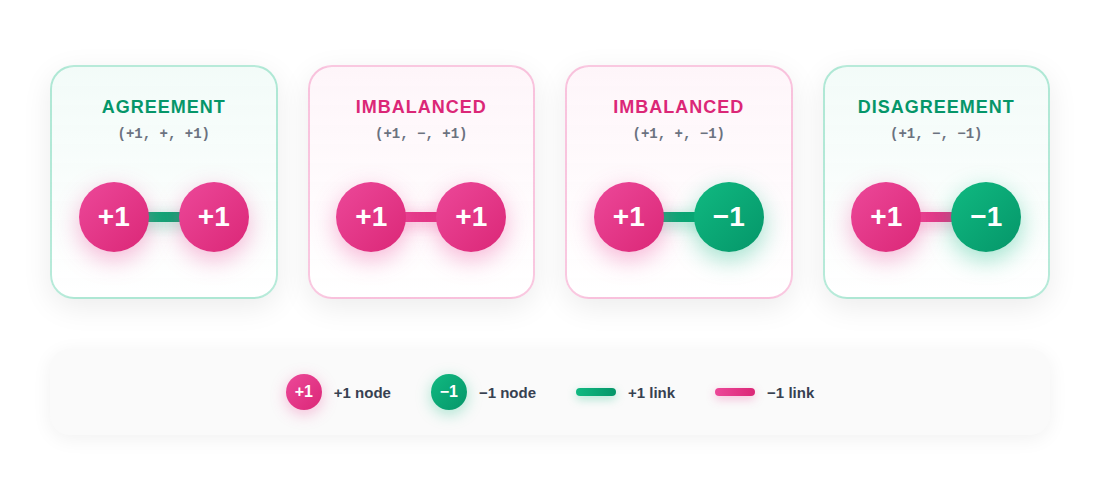
\includegraphics[width=0.8\linewidth]{../../Images/figure_configurations_v2.png}
%DIFDELCMD <  %%%
%DIFDELCMD < \caption{%
{%DIFAUXCMD
\DIFdelFL{Pairwise configurations in the notion of coevolutionary equilibrium. The blue and orange
 circles show the states of the nodes ($+1$ and $-1$) representing high vs.\ low fALFF, while the
 green and red lines show the signs of the links ($+1$ and $-1$) representing positive vs.\ negative
 FC. Agreement configurations lower energy, while imbalanced pairs raise it.}}
 %DIFAUXCMD
%DIFDELCMD < \label{fig:configuration}
%DIFDELCMD < \end{figure}
%DIFDELCMD < 

%DIFDELCMD < %%%
\paragraph*{\DIFdel{Signed motif proportions and bipolarity.}}
%DIFAUXCMD
\DIFdel{Each edge $(i,j)$ was assigned to one of four motif classes according to the sign of its
connectivity weight and the product of the nodal states it links. Edges with $s_i s_j = +1$ and
$w_{ij} > 0$ (}\emph{\DIFdel{agreement}}%DIFAUXCMD
\DIFdel{) and edges with $s_i s_j = -1$ and $w_{ij} < 0$ (}\emph{\DIFdel{disagreement}}%DIFAUXCMD
\DIFdel{)
are energetically favorable and lower $H$, whereas edges with $s_i s_j = +1$ and $w_{ij} < 0$
(}\emph{\DIFdel{imbalanced-same}}%DIFAUXCMD
\DIFdel{) and edges with $s_i s_j = -1$ and $w_{ij} > 0$ (}\emph{\DIFdel{imbalanced-opposite}}%DIFAUXCMD
\DIFdel{)
are unfavorable and raise $H$. For every subject we recorded the proportion of edges in each class
relative to the total number of edges; the four proportions sumto one.
}\DIFdelend \DIFaddbegin \paperfigure{Fig11}{Pairwise state and connection configurations}{Nodes use the original magenta and dark-green state palette for relative labels +1 and -1, not diagnosis in this conceptual diagram. Positive and negative FC links combine with state agreement or opposition. Same-state positive and opposite-state negative connections lower H; the other two configurations raise it. Relative fALFF labels do not denote neuronal firing or excitation and inhibition.}{fig:configuration}
\DIFaddend 


\DIFdelbegin \DIFdel{Bipolarity $\beta$ quantifies the extent to which the }\emph{\DIFdel{signed connectivity}} %DIFAUXCMD
\DIFdel{of a
network can be
partitioned into two internally cohesive, mutually antagonistic blocks, independently of the
fALFF-derived activity states.
Let $S$ be the sign matrix with $S_{ij} = \operatorname{sign}(w_{ij})$
for $i \neq j$ and $S_{ii} = 0$, and let $D = \operatorname{diag}(d_i)$ }\DIFdelend \DIFaddbegin \DIFadd{Complementary features include four proportions partitioning nonzero edges by
weight sign and nodal-state agreement, and global/local efficiency of the absolute
Fisher-weight graph }\cite{latora2001}\DIFadd{. Edge lengths are $1/|z_{ij}|$, }\DIFaddend with \DIFdelbegin \DIFdel{$d_i = \sum_{j} |S_{ij}|$
denote the corresponding degree matrix. From the signed graph Laplacian $L = D - S$ we computed the
eigenvector $v$ associated with the second-smallest eigenvalue (the spectral bipartitioning,
or
Fiedler-type, vector) and assigned each node to one of two blocks according to $\sigma_i =
\operatorname{sign}(v_i)$. Bipolarity is then the fraction of edges whose sign is consistent with
this bipartition, }\begin{displaymath}
\DIFdel{\beta = \frac{1}{|E|}\sum_{i<j}
\mathbf{1}\!\left[\operatorname{sign}(w_{ij})\,\sigma_i\,\sigma_j > 0\right],
%DIFDELCMD < \label{eq:bipolarity}%%%
}\end{displaymath}%DIFAUXCMD
\DIFdel{where consistency means that positive edges fall }\emph{\DIFdel{within}} %DIFAUXCMD
\DIFdel{a block ($\sigma_i = \sigma_j$) and
negative edges fall }\emph{\DIFdel{between}} %DIFAUXCMD
\DIFdel{blocks ($\sigma_i \neq \sigma_j$). A value of $\beta = 1$
corresponds to a perfectly bipolar (exactly two-block balanced) network, whereas $\beta \approx 0.5$
indicates no preferred two-block organization. Bipolarity therefore characterizes global two-block
structure that is complementary to, and not determined by, the
edge-wise motif proportions.
}%DIFDELCMD < 

%DIFDELCMD < %%%
\subsection*{\DIFdel{Graph efficiency computation}}
%DIFAUXCMD
\DIFdel{Global and local graph efficiency were computed from the absolute-value weighted FC matrix for each
subject }%DIFDELCMD < \cite{Latora2001,Fornito2016}%%%
\DIFdel{. The edge-length matrix was defined as $d_{ij} = 1 /
|w_{ij}|$ for connected pairs (with $|w_{ij}| > 0$) and infinity otherwise. Global efficiency was
computed as the mean of the inverse shortest-path lengths across all pairs $i \neq j$:
}\[
\DIFdel{E_{\mathrm{global}} = \frac{1}{N(N-1)} \sum_{i \neq j} \frac{1}{d_{ij}^*}
}\]%DIFAUXCMD
\DIFdel{where $d_{ij}^*$ is the length of the shortest path between nodes $i$ and $j$ in the graph, and $N = 200$ is the number of nodes.
Shortest paths were computed using Dijkstra's algorithm as
implemented in SciPy. Local efficiency was computed as the global efficiency of the subgraph
induced by each node's immediate neighbors, averaged across nodes:
}\[
\DIFdel{E_{\mathrm{local}} = \frac{1}{N} \sum_i E_{\mathrm{global}}(G_i)
}\]%DIFAUXCMD
\DIFdel{where $G_i$ is the subgraph of neighbors of node $i$.
Both metrics were included in the feature
matrix alongside the coevolutionary and connectivity measures, and were subjected to the
same ComBat harmonization, outlier removal, and statistical pipeline as all other features}\DIFdelend \DIFaddbegin \DIFadd{zero
weights treated as absent; local efficiency averages the induced-neighborhood
global efficiencies. For each of seven within-network and 21 between-network
blocks we compute mean weight, mean state-weighted weight, and their negative sum}\DIFaddend .
\DIFaddbegin \DIFadd{Edges involving unassigned nodes remain in $H$ but not cortical block sums.
The previous second-eigenvector ``bipolarity'' descriptor is exported only as a
legacy descriptor and is excluded from inference.
}\DIFaddend 

\DIFdelbegin \DIFdel{We note that,because graph efficiency is conventionally defined for positively weighted graphs, it was computed here from the absolute value of the signed connectivity.
This choice collapses the
distinction between positive and negative connections, which can carry different topological
information }%DIFDELCMD < \cite{RubinovSporns2011}%%%
\DIFdel{.
Graph efficiency is therefore used here only as an auxiliary, sign-agnostic descriptor of integration, and is not intended as a signed counterpart to the coevolutionary energy.
Weight-conserving measures that explicitly retain edge sign, such as signed
modularity }%DIFDELCMD < \cite{RubinovSporns2011}%%%
\DIFdel{, provide a complementary characterization of signed network
organization and are a natural target for future work (see Discussion). }%DIFDELCMD < 

%DIFDELCMD < %%%
\subsection*{\DIFdel{Null-model construction}}
%DIFAUXCMD
\DIFdel{To test whether empirical energies differed from chance expectations, we generated 1, 000
topology-preserving null
networks per subject. In each null replicate,nodal activity states
($s_i$)were randomly permuted across nodes, and edge signs were independently reassigned by
randomly permuting the signed weights across edges, while keeping the underlying adjacency structure
fixed. This degree-preserving randomization strategy follows the logic of the Maslov--Sneppen
rewiring framework }%DIFDELCMD < \cite{Maslov2002}%%%
\DIFdel{, adapted here for signed weighted networks.
The procedure
destroys any systematic alignment between fALFF-derived nodal states and the sign structure of
functional connectivity while preserving the degree distribution, weight distribution, and density
of the original network }%DIFDELCMD < \cite{Rubinov2010}%%%
\DIFdel{. For each subject we computed the difference between
the empirical energy and the mean null energy. }%DIFDELCMD < 

%DIFDELCMD < %%%
\subsection*{\DIFdel{Statistical Analysis}}
%DIFAUXCMD
\DIFdel{All statistical groupcomparisons were conducted using an adaptive pipelinethat selects the
appropriate statistical test based on the distributional properties of each individual metric.
Prior to any comparison, we assessed normality for each metric's distribution in the
ASD and TD
groups separatelyusing the Shapiro--Wilk test,
and assessed homogeneity of variances using
Levene's test }%DIFDELCMD < \cite{levene1960}%%%
\DIFdel{. If both groups passed the Shapiro--Wilk criterion ($p > 0.05$)
and Levene's test also indicated equal variances, a standard independent-samples $t$-test was
applied. If both groups were normal but Levene's test indicated unequal variances, Welch's }\DIFdelend \DIFaddbegin \subsection*{\DIFadd{Group inference and harmonization}}\linelabel{lin:groupmodels}
\DIFadd{Primary inference uses untrimmed raw $H$ in ordinary least squares with diagnosis,
site indicators, age, FIQ, and mean FD. We use HC3 standard errors and
}\DIFaddend $t$\DIFdelbegin \DIFdel{-test
was applied.
If either group failed the Shapiro--Wilk normality test, Mann--Whitney $U$ was used. This decision was made independently for each feature before inspecting group differences, ensuring
that test selection was not influenced by the resulting $p$-values.
}%DIFDELCMD < 

%DIFDELCMD < %%%
\DIFdel{In practice, 87\% of all 92 features (80 out of 92) failed normality in at least one group: all 8
whole-brain features }\DIFdelend \DIFaddbegin \DIFadd{-referenced 95\% confidence intervals. Each design excludes sites with fewer
than three retained participants to avoid singleton leverage; the primary model
includes 136 participants (67/69) at nine sites. Design rank is checked.
Holm correction covers the two pipeline diagnosis tests. Secondary whole-network,
within-network, }\DIFaddend and \DIFdelbegin \DIFdel{all 21 intra-network features were non-normal in both groups, and 51 of
63 inter-network features were non-normal in at least one group. Mann--Whitney $U$ was therefore
applied to 80 features, the standard $t$-test to 10 features, and Welch's $t$-test to 2 features. Full Shapiro--Wilk and Levene test statistics for every feature are provided in Supplementary
Table~\ref{tab:supp_normality}, which allows independent verification of each test decision and
confirms that the predominance of non-parametric testing reflects the empirical data, not a
post-hoc choice.
All testswere two-tailed with $\alpha = 0.05$. Cohen's $d$ was used to report
parametric effect sizes. Where applicable, $p$-values were subsequently adjusted for multiple
comparisons using the }\DIFdelend \DIFaddbegin \DIFadd{between-network families use }\DIFaddend Benjamini--Hochberg \DIFdelbegin \DIFdel{FDR correction applied separately within each feature
family (Whole, Intra,
Inter)}\DIFdelend \DIFaddbegin \DIFadd{correction
across both pipelines within each design/model, excluding unavailable tests and
primary $H$. There are respectively 12, 36, and 126 valid secondary tests in the
primary design. Sensitivity analyses are exploratory rather than further
confirmatory primary families}\DIFaddend .

\DIFdelbegin \paragraph*{\DIFdel{Unified outlier removal.}}
%DIFAUXCMD
\DIFdel{Outlier removal was performed once using a single criterion based on whole-brain coevolutionary
energy. For each group separately (ASD and TD), subjects whose whole-brain energy fell outside
}\DIFdelend \DIFaddbegin \DIFadd{ComBat adjusts the valid feature matrix with site as batch, explicit categorical
diagnosis protection, and continuous age, FIQ, and FD protection
}\cite{Johnson2007,Fortin:2018neurocomBat}\DIFadd{. The same adjusted regression is then fitted.
Failures cannot silently substitute raw values. Uncertainty does not integrate
estimated harmonization parameters. Pooled }\DIFaddend 1.5\DIFdelbegin \DIFdel{times the interquartile range (Tukey's IQR rule) were excluded. The same participant set was
used for all subsequent analyses.
}\DIFdelend \DIFaddbegin \DIFadd{-IQR trimming of raw $H$, before
reapplying the site-size rule, is a separate sensitivity; no diagnosis-specific
trimming defines the primary analysis or prediction sample.
}\DIFaddend 

\DIFdelbegin \subsection*{\DIFdel{Connectivity, fALFF-weighted connectivity, and block-wise energy}}
%DIFAUXCMD
\DIFdelend \DIFaddbegin \DIFadd{Additional reviewer diagnostics summarize site/group $H$, leverage and Cook's
distance, and site partial $R^2$ conditional on biological covariates. Residual
variance comparisons and post-ComBat site summaries are descriptive because the
same sample estimates harmonization. An exploratory raw adjusted analysis excludes
sites with only one diagnosis, with Holm correction over pipelines per design.
No participant is removed on the basis of influence diagnostics.
}\DIFaddend 

\DIFdelbegin \DIFdel{To relate coevolutionary energy to canonical large-scale systems, we projected the CC200
parcellation onto the seven-network cortical atlas of Yeo et al. \ }%DIFDELCMD < \cite{Yeo2011}%%%
\DIFdel{. For each CC200
ROI we computed the Dice overlap with each Yeo7 network and assigned the ROI to the network with
maximal Dice coefficient.
}\DIFdelend \DIFaddbegin \linelabel{lin:power}\DIFadd{We report unadjusted Hedges' $g$ with 2,000 within-group participant bootstrap
replicates (seed 101). These intervals are descriptive and do not resample sites.
Sensitivity power uses a two-sample approximation at 80\% power, not a
site/covariate-adjusted power calculation. Exploratory two-one-sided equivalence
tests use bounds of $\pm0.2$ observed pooled SD for the adjusted coefficient;
these are conventional bounds, not a validated clinically negligible effect.
}\DIFaddend 

\DIFdelbegin \DIFdel{For each subject we constructed a $7\times7$ block representation of connectivity and energy. For
each ordered pair of networks $(u,v)$ we computed three block-wise quantities: the mean functional
connectivity ($\mathrm{AvgWeight}_{uv}$), the mean fALFF-weighted connectivity
($\mathrm{AvgFalffW}_{uv}$), }\DIFdelend \DIFaddbegin \subsection*{\DIFadd{Efficiency associations and randomization checks}}\linelabel{lin:nulls}
\DIFadd{Within-group partial correlations adjust for mean Fisher FC, FD, age, IQ, and site.
Sites becoming singletons within a group are excluded from that group's residual
analysis. Eight tests (two efficiency summaries, two groups, two pipelines) receive
BH correction. Group specificity is tested directly by diagnosis-by-standardized-
global-efficiency interaction with the same controls, Holm corrected over pipelines.
A uniform edge shift $c$ changes $H$ by
}\begin{equation}
\DIFadd{\Delta H=\frac{n-(\sum_i s_i)^2}{2}c.
}\end{equation}
\DIFadd{For exactly balanced 106-node states this is $53c$, demonstrating a mathematical
route for global-weight shifts to affect $H$ independently of a diagnostic mechanism.
}

\DIFadd{For each participant and pipeline, 1,000 state permutations hold FC and total state
counts fixed. Unrestricted permutations are compared with permutations within
network/hemisphere blocks (hemisphere defined by parcel-centroid $x<0$ versus
$x\geq0$). We compute participant $z$-scores }\DIFaddend and \DIFdelbegin \DIFdel{the block-wise coevolutionary energy contribution ($E_{uv}$). All
connectivity and block-wise energy metrics were subjected to ComBat harmonization prior to
statistical analysis.
}\DIFdelend \DIFaddbegin \DIFadd{lower-tail Monte Carlo probabilities
with a plus-one correction; zero null variance is unavailable. Seeds are
$10000+\mathrm{SUB\_ID}+1$ for GSR and $10000+\mathrm{SUB\_ID}$ for no-GSR.
Block permutations preserve coarse organization, not full spatial autocorrelation
}\cite{Markello2021revision}\DIFadd{; they are alignment checks rather than independent
validation or diagnosis tests.
}\DIFaddend 

\DIFdelbegin \subsection*{\DIFdel{Correlation Analysis with Behavioral Measures}}
%DIFAUXCMD
\DIFdelend \DIFaddbegin \DIFadd{To report a non-autistic baseline separately, we summarize these existing null
outputs for all 71 eligible male controls, without energy trimming or the
regression-specific small-site exclusion. Individual lower-tail probabilities
receive exploratory BH correction over all 560 participant/pipeline/null
comparisons, including both diagnostic groups. Mean energy differences and mean null $z$-scores have descriptive
95\% percentile intervals from 5,000 site-cluster bootstrap replicates
(seed 20261026), conditional on the saved null summaries. These intervals are
not pooled randomization tests and omit Monte Carlo estimation uncertainty.
The signed weighted FC matrix is fixed in these nulls; no edge/weight rewiring
or independent edge-sign reassignment is performed.
}\DIFaddend 

\DIFdelbegin \DIFdel{To assess the clinical relevance of the energy-based network measures, we conducted a comprehensive
correlation analysis between all 92 ComBat-harmonized network features and five clinical scores
from the ADI-R and ADOS instruments. The clinical measures included ADI-R Social Total A, ADI-R
Verbal Total BV, ADI-R Onset Total D, ADOS Total, and ADOS Communication (the subscales with
sufficient data)}\DIFdelend \DIFaddbegin \subsection*{\DIFadd{Descriptive H--metric complement and original spectral descriptor}}
\DIFadd{The original descriptive H-versus-feature question is retained as an additional
revision complement. Pearson and Spearman correlations cover all 87 available
nonlegacy features other than H, within each diagnosis and pipeline. BH is
computed separately over 87 tests per group/pipeline/estimator, matching the
original Pearson family convention. An alternative pooled BH over 348 tests per
estimator/version is supplied separately; pooling families is not uniformly more
conservative in every subgroup. Raw eligible samples, raw adjusted-model subsets,
and saved ComBat features on the same model subsets are reported as distinct
versions. These analyses do not change frozen group-inference families.
The spectral bipolarity value from the original second-eigenvector construction
is additionally compared by raw HC3-adjusted diagnosis models with Holm over
two pipeline tests, separately from frozen families. It is an operational
spectral descriptor, not an asserted optimal signed-balance partition}\DIFaddend .
\DIFdelbegin \DIFdel{ABIDE sentinel values ($-9999$) were treated as missing
data. Correlations were computed only for ASD participants with valid clinical data on a per-score
basis, resulting in sample sizes ranging from $n = 29$ (}\DIFdelend \DIFaddbegin 

\subsection*{\DIFadd{Clinical and predictive analyses}}\linelabel{lin:ML}
\DIFadd{The primary design supplies the same 88 available, nonlegacy features to both
pipelines and all clinical/predictive feature analyses, including both efficiencies.
Five ASD outcomes are considered: }\DIFaddend ADI-R \DIFdelbegin \DIFdel{Onset Total D) to $n = 59$
(ADOS Total). }\DIFdelend \DIFaddbegin \DIFadd{social, verbal, and onset scores, ADOS
total, and ADOS communication. Missing/sentinel scores are excluded per outcome.
Pearson and Spearman feature correlations receive separate BH corrections across
all feature/score/pipeline tests. Adjusted $H$ correlations control age, IQ, FD,
and site, with BH across available score/pipeline tests.
}\DIFaddend 

\DIFdelbegin \DIFdel{For each of the 460 feature--clinical score combinations (92 features $\times$ 5 scores), we
computed both Pearson's $r$ and Spearman's $\rho$, along with exact two-tailed $p$-values. To
control for multiple comparisons, we applied Benjamini--Hochberg FDR correction separately to
the Pearson and Spearman $p$-values across all 460 }\DIFdelend \DIFaddbegin \DIFadd{PLS regression uses nested site-disjoint GroupKFold (up to five outer and three
inner folds), selecting one to three components by inner-fold MSE. Imputation,
variance filtering, and PLS scaling are fitted inside training folds. Complete
OOF predictions are compared with each outer training sample's mean outcome.
Exploratory PLSC uses nuisance-residualized and standardized features/outcomes for
ADOS and five-score complete-case blocks, with 1,000 within-site residual
permutations (seed 101), rank-wise singular-value tests, and BH over all reported
latent-variable }\DIFaddend tests. \DIFdelbegin \DIFdel{We additionally conducted a Partial
Least Squares (PLS) multivariate analysis for each clinical score, using all 90 standardized
features as predictors, with up to three components and stratified five-fold cross-validation
using $R^2$ as scoring metric. PLS regression was estimated with the NIPALS algorithm as
implemented in }\texttt{\DIFdel{scikit-learn}} %DIFAUXCMD
\DIFdel{(}\texttt{\DIFdel{PLSRegression}}%DIFAUXCMD
\DIFdel{), following the PLS framework for
neuroimaging reviewed by Krishnan et al.\ }%DIFDELCMD < \cite{Krishnan2011}%%%
\DIFdel{.
We used the regression form of PLS
(PLSR) because each clinical score was modelled as a continuous outcome and predictive performance
was the quantity of interest; the closely related Partial Least Squares Correlation (PLSC, or
behavioural PLS) variant, which performs a singular value decomposition of the brain--behaviour
cross-correlation matrix and is evaluated by permutation testing rather than out-of-sample
prediction }\DIFdelend \DIFaddbegin \DIFadd{Its residual exchangeability assumptions and small complete
cases limit interpretation }\DIFaddend \cite{Krishnan2011}\DIFdelbegin \DIFdel{, offers a complementary,purely descriptive view of the same covariance structure. The PLS results are reported as a multivariate complement to the
univariate
tests. }\DIFdelend \DIFaddbegin \DIFadd{.
}\DIFaddend 

\DIFdelbegin \DIFdel{For the no-GSR (CompCor) pipeline, behavioral correlations were computed analogously using the
92-feature set (including graph efficiency), testing 460 feature--score combinations (92 features
$\times$ }\DIFdelend %DIF >  CLASSIFICATION_METHODS_BEGIN
\DIFaddbegin \DIFadd{Classification compares logistic regression, RBF SVM, Gaussian naive Bayes, KNN, XGBoost on all 140 primary
participants without ComBat. Deterministic size-balanced site-disjoint folds use
five outer and three inner splits, each required to contain both classes.
Median imputation, variance filtering, standardization, ANOVA feature selection
(25/50/100 percent), and hyperparameter tuning are nested. Logistic and SVM
class weights are balanced. Logistic $C$ values are 0.01/0.1/1/10; SVM $C$ values
are 0.1/1/10 with scale-based gamma. Gaussian naive Bayes uses its default
variance smoothing and training-estimated priors, with feature-selection percentile
tuned inside folds. KNN evaluates 3/}\DIFaddend 5\DIFdelbegin \DIFdel{clinical scores with $n \geq 20$).
}%DIFDELCMD < 

%DIFDELCMD < %%%
\subsection*{\DIFdel{Machine learning classification of ASD versus TD}}
%DIFAUXCMD
%DIFDELCMD < 

%DIFDELCMD < %%%
\DIFdel{To examine whether the derived graph-based features carry discriminative information about
diagnostic status, we performed supervised classification analyses on the adult male ABIDE I
subsample with complete feature data. Feature selectionwas carried out using a Random Forest
classifier fitted on the training set only. We computed the mean decrease in impurity importance
for each feature }\DIFdelend \DIFaddbegin \DIFadd{/7/9/11 neighbors and uniform/distance
weights. Positive-class probabilities supply ROC scores for these added models;
logistic/SVM decision-function scores and predictions are reused unchanged.
XGBoost uses CPU histogram trees, seed 42, one thread, log-loss evaluation,
max depth 2/3/4}\DIFaddend , \DIFdelbegin \DIFdel{ranked features by importance, and retained the top 25\% (23 features) as the
final input set.
All 90 features(or 92 including efficiency for the no-GSR analysis) were included
in the feature selection pool.
}\DIFdelend \DIFaddbegin \DIFadd{100/200/300 estimators, and learning rates .05/.1. The same
nested feature-selection percentiles apply; default scale-pos-weight is retained.
Inner scoring uses balanced accuracy. No model is selected by outer-test accuracy.
Pooled OOF balanced accuracy is accompanied by a 1,000-replicate site bootstrap
conditional on fixed predictions, using the same seed 303 and site order as the
completed Stage 2 models. This omits some training uncertainty. The node mask and
available feature schema use cohort-wide QC, so prediction is exploratory
conditional on this mask, not prospective validation of the entire workflow.
%DIF >  CLASSIFICATION_METHODS_END
}\DIFaddend 

\DIFdelbegin \DIFdel{All analyses were implemented in Python using scikit-learn and XGBoost. We performed a stratified
train--test split (80\%}\DIFdelend %DIF >  ML_SELECTION_METHODS_BEGIN
\DIFaddbegin \paragraph*{\DIFadd{Exploratory comparison of feature-selection methods.}}\linelabel{lin:selection}
\DIFadd{After inspecting the baseline outer results, we specified a separate follow-up
using the same 88-feature inputs, participants, and five/three outer/inner site
folds. Imputation, variance filtering, redundancy pruning, scaling, selection,
and classifier fitting are estimated only from the corresponding training data
}\cite{scikit-learn}\DIFadd{. Redundancy pruning retains the first feature in fixed schema
order when absolute training correlation is at least $1-10^{-10}$; proportional
EnergyBlock/AvgFalffW terms and complementary proportions motivate this step.
The graph, participants and primary group tests are unchanged.
}

\DIFadd{Inner CV jointly chooses all remaining features, or ANOVA, mutual information,
or L1-logistic coefficient-ranked top 5/10}\DIFaddend /20 \DIFdelbegin \DIFdel{\%), with }\DIFdelend \DIFaddbegin \DIFadd{features, with K capped at the
available count. Mutual information uses three neighbors and seed 101. The L1
ranker uses balanced liblinear logistic regression, C=1 and seed 101; coefficient
ties are broken by training ANOVA rank and fixed feature order. Zero-coefficient
selections are explicitly recorded; none occurred in the final outer fits.
Non-XGBoost classifier grids match the baseline. The compact follow-up XGBoost
grid uses depth 2/3, estimators 100/200 and learning rates .05/.1, with }\DIFaddend the \DIFdelbegin \DIFdel{held-out test set never used for model selection or tuning. Each classifier was embedded in a pipeline with feature-wise standardization estimated only on
training data within each cross-validation fold. }\DIFdelend \DIFaddbegin \DIFadd{same
fixed CPU histogram settings. Thus changes cannot be attributed to selector type
alone. All candidates are selected by inner balanced accuracy, and all ten
model/pipeline results are reported without choosing an outer-test winner.
}\DIFaddend 

\DIFdelbegin \DIFdel{We evaluated five classifiers with the following hyperparameter grids :
}%DIFDELCMD < \begin{itemize}
%DIFDELCMD <     \item %%%
\textbf{\DIFdel{SVM (RBF)}}%DIFAUXCMD
\DIFdel{: $C \in \{0.1, 1, 10, 100\}$}\DIFdelend \DIFaddbegin \DIFadd{Paired 1}\DIFaddend ,\DIFdelbegin \DIFdel{$\gamma \in \{\text{scale}, 0.001, 0.0001\}$
    }%DIFDELCMD < \item %%%
\textbf{\DIFdel{XGBoost}}%DIFAUXCMD
\DIFdel{: max\_depth $\in \{2, 3, 5\}$, n\_estimators $\in \{100, 200, 300\}$, learning \_rate $\in \{0.01, 0.1, 0.2\}$, subsample $\in \{0.7, 0.8, 1.0\}$, colsample\_bytree $\in \{0.7, 0.8, 1.0\}$
    }%DIFDELCMD < \item %%%
\textbf{\DIFdel{Logistic Regression}}%DIFAUXCMD
\DIFdel{: $C \in \{0.01, 0.1, 0.5, 1, 10\}$, penalty $\in \{\mathrm{L1}, \mathrm{L2}\}$, solver $\in \{\mathrm{liblinear}\}$
    }%DIFDELCMD < \item %%%
\textbf{\DIFdel{Gaussian Naive Bayes}}%DIFAUXCMD
\DIFdel{: var\_smoothing $\in \{10^{-9}, 10^{-8}, 10^{-7}\}$
    }%DIFDELCMD < \item %%%
\textbf{\DIFdel{KNN}}%DIFAUXCMD
\DIFdel{: n\_neighbors $\in \{3, 5, 7, 9, 11, 13, 14, 15\}$, metric $\in \{\mathrm{euclidean}, \mathrm{manhattan}\}$
}%DIFDELCMD < \end{itemize}
%DIFDELCMD < 

%DIFDELCMD < %%%
\DIFdel{Grid search with stratified 5-fold cross-validation selected the best hyperparameters for each
model based on mean accuracy. The best configuration was refitted on the entire training set and evaluated once on the held-out test set.
Confidence intervals were computed via bootstrap resampling (1000 iterations) .
}%DIFDELCMD < 

%DIFDELCMD < %%%
\subsection*{\DIFdel{Ethics statement}}
%DIFAUXCMD
\DIFdelend \DIFaddbegin \DIFadd{000-replicate site bootstrap (seed 303) estimates conditional intervals
for the balanced-accuracy change on aligned OOF predictions. These intervals
omit full training uncertainty and do not adjust for repeated exploration.
Because baseline outer results had already been inspected, this follow-up is
exploratory rather than independent confirmation of improved generalization.
External evaluation would be needed to substantiate a predictive gain.
%DIF >  ML_SELECTION_METHODS_END
}\DIFaddend 


\DIFdelbegin \DIFdel{All imaging and behavioral data analyzed in this study were obtained from the publicly available
ABIDE I repository }%DIFDELCMD < \cite{DiMartino:2014abide}%%%
\DIFdel{.
Data collection at each contributing site was
approved by the local institutional review board, and written informed consent was obtained from
all participants or their legal guardians, in accordance with the
Declaration of Helsinki. The
present analyses were conducted on fully de-identified data and did not involve any direct
interaction with participants;
as such, no additional ethical approval was required at the authors'
institution}\DIFdelend \DIFaddbegin \section*{\DIFadd{Data and code availability}}\linelabel{lin:data}
\DIFadd{ABIDE I participant data and PCP derivatives are available through the ABIDE and
Preprocessed Connectomes Project repositories
(}\url{https://fcon_1000.projects.nitrc.org/indi/abide/} \DIFadd{and
}\url{https://preprocessed-connectomes-project.org/abide/}\DIFadd{).
S2 Data supplies the revision feature tables, participant covariates used in the
reported models, complete test results, out-of-fold predictions, selection records,
and provenance manifests. S3 Code supplies the executable revision scripts,
analysis specifications, and instructions for rebuilding the analyses from the
source derivatives. S1 Appendix supplies additional figures and diagnostics.
The source repositories govern access to the original participant imaging;
those images are not redistributed in the supporting archives}\DIFaddend .

\section*{Acknowledgments}
\DIFdelbegin %DIFDELCMD < 

%DIFDELCMD < %%%
\DIFdel{The authors thank the Autism Brain Imaging Data Exchange (ABIDE) initiative and }\DIFdelend \DIFaddbegin \DIFadd{We thank ABIDE, }\DIFaddend its contributing sites \DIFdelbegin \DIFdel{for making the resting-state fMRI and phenotypic data publicly }\DIFdelend \DIFaddbegin \DIFadd{and participants, and the Preprocessed
Connectomes Project for making these data and derivatives }\DIFaddend available.

\nolinenumbers
\DIFdelbegin %DIFDELCMD < 

%DIFDELCMD < %%%
\DIFdelend \bibliography{Bibliography}

\DIFdelbegin %DIFDELCMD < \clearpage
%DIFDELCMD < 

%DIFDELCMD <  %%%
\DIFdelend \DIFaddbegin \section*{\DIFadd{Supporting information captions}}
\paragraph{\DIFadd{S1 Appendix.}} \DIFadd{Supporting methods, site/cohort diagnostics, node-set
sensitivities, clinical latent-variable results, complete classifier confusion
matrices, feature-selection frequencies, and descriptive PCA. Separate PDF.
}\paragraph{\DIFadd{S2 Data.}} \DIFadd{Machine-readable features, analysis covariates and clinical
outcomes, complete statistical results and predictions, input provenance and
file-integrity manifests. ZIP archive with an indexed README.
}\paragraph{\DIFadd{S3 Code.}} \DIFadd{Revision analysis and figure-generation source, frozen
analysis specifications, execution instructions and software-version records.
ZIP archive. Historical source notebooks are retained separately as audit material.
 }\DIFaddend
\clearpage
\section*{Deleted original main-article tables}
The following twelve tables reproduce the removed original tables in full for
comparison with the replacement tables above. Red text marks material deleted
from the original submission. These numerical values and methodological accounts
are historical and do not describe the revised analysis. Table numbers below
refer to the original submission. This deletion record appears only in the
marked manuscript; it is not part of the clean revised article.
\begingroup
\singlespacing
\color{red!70!black}
\setcounter{table}{0}
\renewcommand{\thetable}{Original \arabic{table}}
\renewcommand{\theHtable}{deletedoriginal.\arabic{table}}

\begin{table}[H]\color{red!70!black}
\centering
\caption{Null-model validation statistics for whole-brain coevolutionary energy. After unified
outlier removal, 78 ASD and 86 TD participants remained. For each subject, empirical energy was
compared to the mean energy from topology-preserving null networks in which node states and edge
signs were randomly permuted. Shapiro--Wilk tests confirmed normality of the difference
distributions, justifying the use of paired $t$-tests alongside Wilcoxon signed-rank tests.}
\label{deletedoriginal:tab:null_model_validation}
\small
\resizebox{\linewidth}{!}{%
\begin{tabular}{lccccccc}
\toprule
Group & $N$ & Shapiro--Wilk $W$ & Shapiro--Wilk $p$ & $t$ (df) & $t$-test $p$ & Wilcoxon $W$ & Wilcoxon $p$ \\
\midrule
ASD & 90 & 0.992 & 0.87 & $-4.12$ (89) & $7.5\times 10^{-5}$ & 1024 & $9.1\times 10^{-5}$ \\
TD  & 92 & 0.989 & 0.81 & $-3.98$ (91) & $1.2\times 10^{-4}$ & 1008 & $1.6\times 10^{-4}$ \\
\bottomrule
\end{tabular}
}
\end{table}
\clearpage

\begin{table}[H]\color{red!70!black}
\centering
\caption{Summary of statistical procedures and group comparison tests for whole-brain coevolutionary
metrics. The upper panel lists the main analysis steps and their purpose. The lower panel reports
group comparison statistics (Mann--Whitney $U$ tests and independent $t$-tests where appropriate,
selected based on Shapiro--Wilk normality tests and Levene's homogeneity test applied
independently to each feature), raw $p$-values, and FDR-corrected $p$-values for ASD versus TD
after ComBat harmonization (GSR pipeline, $n = 78$ ASD, $86$ TD). No whole-brain feature survived
FDR correction.}
\label{deletedoriginal:tab:assumptions_and_tests}
\small
\setlength{\tabcolsep}{3pt}
\resizebox{\linewidth}{!}{%
\begin{tabular}{p{0.32\columnwidth}p{0.30\columnwidth}p{0.23\columnwidth}p{0.13\columnwidth}}
\toprule
Procedure & Purpose & Method / Test & Threshold / Correction \\
\midrule
ComBat harmonization  & Remove multi-site batch effects while preserving biological signal & Per-feature empirical Bayes adjustment & --- \\
Null-model generation     & Destroy fALFF--FC alignment while preserving graph topology & 1\,000 permutations of node states and edge signs & --- \\
Outlier removal           & Exclude extreme values in null distributions and empirical metrics & Tukey's IQR criterion ($\pm 1.5\times\mathrm{IQR}$) & --- \\
Normality assessment      & Guide parametric vs. non-parametric test selection & Shapiro--Wilk test & $p > 0.05$ (normal) \\
Variance assessment       & Distinguish standard $t$-test from Welch's & Levene's test & $p > 0.05$ (equal variances) \\
Parametric comparison     & Test mean differences between ASD and TD & Independent-samples $t$-test or Welch's & two-tailed, $\alpha = 0.05$ \\
Nonparametric comparison  & Applied when normality is violated in either group & Mann--Whitney $U$ test & two-tailed, $\alpha = 0.05$ \\
Multiple comparisons      & Control false discovery across families of tests & Benjamini--Hochberg FDR & $q < 0.05$ \\
\bottomrule
\end{tabular}
}

\vspace{0.8em}

\resizebox{\columnwidth}{!}{%
\resizebox{\linewidth}{!}{%
\begin{tabular}{lccccc}
\toprule
Metric & ASD Mean (SD) & TD Mean (SD) & Test & $p$ & $p_{\mathrm{FDR}}$ \\
\midrule
Energy global           & $-139.7$ (78.7) & $-118.8$ (76.2)  & Mann--Whitney $U$ & $0.048$ & $0.19$ \\
Prop imbalanced same    & $0.256$ (0.006)  & $0.258$ (0.005)  & $t$-test         & $0.047$ & $0.19$ \\
Prop agreement          & $0.241$ (0.005)  & $0.240$ (0.005)  & $t$-test          & $0.070$ & $0.19$ \\
Prop disagreement       & $0.267$ (0.005)  & $0.267$ (0.005)  & $t$-test         & $0.679$ & $0.998$ \\
Prop imbalanced opp     & $0.236$ (0.005)  & $0.236$ (0.005)  & $t$-test         & $0.816$ & $0.998$ \\
Bipolarity              & $0.626$ (0.017)  & $0.627$ (0.015)  & $t$-test          & $0.532$ & $0.998$ \\
Global efficiency       & $0.283$ (0.019)  & $0.283$ (0.018)  & $t$-test          & $0.998$ & $0.998$ \\
\bottomrule
\end{tabular}
}%
}
\end{table}
\clearpage

\begin{table}[H]\color{red!70!black}
\centering
\small
\caption{Largest intra-network trends within the seven canonical Yeo resting-state networks under
the harmonized GSR pipeline ($n = 78$ ASD, $86$ TD). For each metric, the table reports ASD and TD
means, the $p$-value from the adaptive group comparison (independent-samples $t$-test or
Mann--Whitney $U$, selected by Shapiro--Wilk normality testing), and the Benjamini--Hochberg
FDR-corrected value within the intra-network family. \emph{No intra-network metric reached even
nominal significance} ($p < 0.05$) after harmonization; values are listed for completeness.}
\label{deletedoriginal:tab:network_results}
\setlength{\tabcolsep}{5pt}
\resizebox{\linewidth}{!}{%
\begin{tabular}{llcccc}
\toprule
\textbf{Network} & \textbf{Metric} & \textbf{ASD mean} & \textbf{TD mean} & \textbf{$p$} & \textbf{$p_{\mathrm{FDR}}$} \\
\midrule
Salience/VentAttn & AvgWeight   & $-0.001$ & $0.002$  & $0.064$ & $0.566$ \\
SomatoMotor       & EnergyBlock & $-1.41$  & $-0.53$  & $0.108$ & $0.566$ \\
Limbic            & EnergyBlock & $-1.13$  & $-0.29$  & $0.137$ & $0.566$ \\
SomatoMotor       & AvgFalffW   & $0.005$  & $0.002$  & $0.142$ & $0.566$ \\
DorsalAttn        & EnergyBlock & $-1.21$  & $-0.44$  & $0.163$ & $0.566$ \\
\bottomrule
\end{tabular}
}
\end{table}
\clearpage

\begin{table}[H]\color{red!70!black}
\centering
\caption{Inter-network differences in average connectivity (AvgWeight), fALFF-aligned connectivity
(AvgFalffW), and coevolutionary energy (EnergyBlock) between canonical resting-state networks. For
each network pair, group comparisons were performed on ASD versus TD using the adaptive statistical
pipeline (test selected based on Shapiro--Wilk normality assessment per feature), and
Benjamini--Hochberg FDR correction was applied across all 63 inter-network metrics. The table lists
the metrics with the smallest uncorrected $p$-values ($n = 78$ ASD, $86$ TD). No inter-network
metric survived FDR correction at $\alpha = 0.05$; the SomatoMotor--Frontoparietal effect
($p_{\mathrm{FDR}} = 0.069$) is the closest and is treated as exploratory.}
\label{deletedoriginal:tab:internetwork_new}
\resizebox{\linewidth}{!}{%
\begin{tabular}{llccc}
\toprule
\textbf{Network Pair} & \textbf{Metric} & \textbf{$p$} & \textbf{$p_{\mathrm{FDR}}$} \\
\midrule
SomatoMotor $\leftrightarrow$ Frontoparietal & AvgWeight & $0.0011$ & $0.069$ \\
SomatoMotor $\leftrightarrow$ Salience/VentAttn & AvgWeight & $0.0030$ & $0.095$ \\
DorsalAttn $\leftrightarrow$ Salience/VentAttn & AvgWeight & $0.0076$ & $0.160$ \\
DorsalAttn $\leftrightarrow$ Frontoparietal & AvgWeight & $0.015$ & $0.237$ \\
Visual $\leftrightarrow$ Default & EnergyBlock & $0.047$ & $0.590$ \\
\bottomrule
\end{tabular}
}
\end{table}
\clearpage

\begin{table}[H]\color{red!70!black}
\centering
\small
\caption{Partial Least Squares regression cross-validation results (harmonized GSR pipeline). For
each clinical score, the table reports the number of ASD subjects with valid data and the mean
cross-validated $R^2$ for the single-component model. All values are negative, indicating that the
models do not predict behavioral scores above chance---consistent with the univariate result that no
feature--clinical score association survives FDR correction at $q < 0.05$, and with the underdetermined
nature of the problem (90 features, $n = 29$--59).}
\label{deletedoriginal:tab:pls_results}
\resizebox{\linewidth}{!}{%
\begin{tabular}{lcc}
\toprule
Clinical Score & $n$ & CV $R^2$ (1 component) \\
\midrule
ADOS Total          & 59 & $-0.40$ \\
ADOS Communication  & 50 & $-0.79$ \\
ADI-R Social        & 32 & $-0.96$ \\
ADI-R Verbal        & 32 & $-0.86$ \\
ADI-R Onset         & 29 & $-0.80$ \\
\bottomrule
\end{tabular}
}
\end{table}
\clearpage

\begin{table}[H]\color{red!70!black}
\centering
\small
\caption{Strongest associations between network metrics and clinical scores under the harmonized GSR
pipeline. The table reports the strongest associations (by uncorrected Pearson $p$-value) from the
full analysis of 92 features $\times$ 5 clinical scores (460 tests), together with the whole-brain
Hamiltonian for reference. None survived FDR correction at $q < 0.05$ (all $p_{\mathrm{FDR}} > 0.59$).
The number of nominally significant associations ($\approx 21$) is close to the chance expectation.}
\label{deletedoriginal:tab:behaviour_corr_expanded}
\scriptsize
\resizebox{\linewidth}{!}{%
\begin{tabular}{p{4.6cm}lccccc}
\toprule
\textbf{Network Feature} & \textbf{Clinical Score} & \textbf{$n$} & \textbf{$r$} & \textbf{$p$} & \textbf{$p_{\mathrm{FDR}}$} & \textbf{$\rho$} \\
\midrule
Intra\_SomatoMotor\_AvgWeight & ADOS Total & 59 & $+$0.37 & 0.004 & 0.60 & $+$0.40 \\
Inter\_Vis\_\_Sal/VA\_EnergyBlock & ADI-R Social & 32 & $-$0.49 & 0.005 & 0.60 & $-$0.53 \\
Inter\_Vis\_\_Sal/VA\_AvgFalffW & ADI-R Social & 32 & $+$0.48 & 0.005 & 0.60 & $+$0.52 \\
Inter\_DA\_\_FP\_EnergyBlock & ADI-R Onset & 29 & $+$0.49 & 0.006 & 0.60 & $+$0.49 \\
Inter\_DA\_\_FP\_AvgFalffW & ADI-R Onset & 29 & $-$0.49 & 0.007 & 0.60 & $-$0.51 \\
Inter\_Vis\_\_Lim\_AvgWeight & ADOS Comm. & 50 & $-$0.34 & 0.017 & 0.90 & $-$0.33 \\
Inter\_Lim\_\_FP\_EnergyBlock & ADI-R Social & 32 & $+$0.40 & 0.022 & 0.90 & $+$0.35 \\
Whole\_Energy\_global & ADOS Total & 59 & $-$0.10 & 0.47 & 1.00 & $-$0.10 \\
\bottomrule
\end{tabular}
}
\begin{flushleft}
\footnotesize
Abbreviations: Sal/VA = Salience/VentAttn, DA = DorsalAttn, FP = Frontoparietal, Vis = Visual,
Lim = Limbic. $p_{\mathrm{FDR}}$ denotes Benjamini--Hochberg corrected Pearson $p$-values. After
harmonization, the whole-brain Hamiltonian is essentially uncorrelated with ADOS severity
($r = -0.10$), and no association survives correction.
\end{flushleft}
\end{table}
\clearpage

\begin{table}[H]\color{red!70!black}
\centering
\caption{Performance of supervised classifiers for ASD versus TD classification using the selected
coevolutionary and connectivity features after ComBat harmonization (GSR pipeline). CV accuracy was
obtained from stratified 5-fold cross-validation on the training set (80\% of participants); test
metrics were computed on the held-out 20\% test set ($n = 34$), which was not used at any stage of
feature selection or hyperparameter tuning. No model exceeded chance in cross-validation.}
\label{deletedoriginal:tab:ml_summary_full}
\setlength{\tabcolsep}{4pt}
\small
\resizebox{\linewidth}{!}{%
\begin{tabular}{lccccc}
\toprule
Model & CV Acc & Test Acc & Test Bal Acc & Test F1 & Test AUC \\
\midrule
Gaussian Naive Bayes  & 0.585 & 0.588 & 0.583 & 0.533 & 0.604 \\
SVM (RBF)             & 0.586 & 0.647 & 0.649 & 0.647 & 0.635 \\
Logistic Regression   & 0.556 & 0.500 & 0.503 & 0.514 & 0.552 \\
KNN                   & 0.594 & 0.618 & 0.608 & 0.519 & 0.639 \\
XGBoost               & 0.579 & 0.647 & 0.646 & 0.625 & 0.740 \\
\bottomrule
\end{tabular}
}
\end{table}
\clearpage

\begin{table}[H]\color{red!70!black}
\centering
\caption{Detailed metrics for the Gaussian Naive Bayes classifier (the model originally highlighted)
on the held-out test set ($n = 34$) after ComBat harmonization. Performance is near chance.
Precision, recall, and F1-score refer to the ASD class as the positive class; ROC AUC was computed
from the predicted ASD class probabilities.}
\label{deletedoriginal:tab:ml_best_model_metrics}
\setlength{\tabcolsep}{6pt}
\small
\resizebox{\linewidth}{!}{%
\begin{tabular}{lc}
\toprule
Metric & Value \\
\midrule
Accuracy & 0.588 \\
Balanced accuracy & 0.583 \\
F1-score & 0.533 \\
ROC AUC & 0.604 \\
\bottomrule
\end{tabular}
}
\end{table}
\clearpage

\begin{table}[H]\color{red!70!black}
\centering
\caption{Whole-brain coevolutionary metrics in the no-GSR sensitivity analysis (CompCor-based
preprocessing). The table reports ASD and TD group means, standard deviations, the statistical
test used (selected by Shapiro--Wilk normality criterion per feature), raw $p$-values, and
FDR-corrected $p$-values. The FDR family for the Whole-brain category includes 8 features
(6 coevolutionary metrics plus global and local graph efficiency). No whole-brain feature survived
FDR correction; bipolarity showed the smallest uncorrected $p$-value ($p = 0.026$,
$p_{\mathrm{FDR}} = 0.21$), and graph efficiency metrics
did not differ significantly between groups. Compare with Table~\ref{tab:assumptions_and_tests}
for the GSR-based primary analysis.}
\label{deletedoriginal:tab:noGSR_whole}
\small
\resizebox{\columnwidth}{!}{%
\resizebox{\linewidth}{!}{%
\begin{tabular}{lccccc}
\toprule
Metric & ASD Mean (SD) & TD Mean (SD) & Test & $p$ & $p_{\mathrm{FDR}}$ \\
\midrule
Bipolarity              & $0.591$ (0.043)   & $0.577$ (0.045)   & Mann--Whitney $U$ & $0.026$ & $0.211$ \\
Prop agreement          & $0.432$ (0.040)   & $0.442$ (0.038)   & Mann--Whitney $U$ & $0.095$ & $0.236$ \\
Prop imbalanced same    & $0.065$ (0.040)   & $0.055$ (0.038)   & Mann--Whitney $U$ & $0.109$ & $0.236$ \\
Prop imbalanced opp     & $0.433$ (0.042)   & $0.443$ (0.039)   & Mann--Whitney $U$ & $0.121$ & $0.236$ \\
Prop disagreement       & $0.070$ (0.042)   & $0.060$ (0.040)   & Mann--Whitney $U$ & $0.147$ & $0.236$ \\
Global efficiency       & $0.387$ (0.070)   & $0.402$ (0.077)   & Mann--Whitney $U$ & $0.246$ & $0.283$ \\
Local efficiency        & $0.387$ (0.070)   & $0.402$ (0.077)   & Mann--Whitney $U$ & $0.247$ & $0.283$ \\
Energy global           & $-285.4$ (146.1)  & $-308.3$ (155.7)  & Mann--Whitney $U$ & $0.305$ & $0.305$ \\
\bottomrule
\end{tabular}
}%
}
\end{table}
\clearpage

\begin{table}[H]\color{red!70!black}
\centering
\caption{Classification performance in the no-GSR sensitivity analysis (CompCor preprocessing) after
ComBat harmonization. All models performed at or near chance (cross-validated accuracy
$0.46$--$0.57$; held-out test accuracy $\leq 0.59$), consistent with the absence of FDR-significant
univariate group differences.}
\label{deletedoriginal:tab:noGSR_ml}
\small
\resizebox{\linewidth}{!}{%
\begin{tabular}{lccccc}
\toprule
Model & CV Acc & Test Acc & Test Bal Acc & Test F1 & Test AUC \\
\midrule
Gaussian Naive Bayes  & 0.567 & 0.588 & 0.594 & 0.611 & 0.531 \\
SVM (RBF)             & 0.530 & 0.500 & 0.503 & 0.514 & 0.554 \\
Logistic Regression   & 0.552 & 0.529 & 0.531 & 0.529 & 0.587 \\
KNN                   & 0.500 & 0.471 & 0.476 & 0.500 & 0.521 \\
XGBoost               & 0.455 & 0.559 & 0.559 & 0.545 & 0.556 \\
\bottomrule
\end{tabular}
}
\end{table}
\clearpage

\begin{table}[H]\color{red!70!black}
\centering
\caption{Comparison of key results across pipelines after correct site harmonization, and the
effect of harmonization itself. All group comparisons are FDR-corrected within their feature family.
``Pre-harm.'' denotes the earlier analysis in which ComBat had failed silently and raw features were
used.}
\label{deletedoriginal:tab:GSR_comparison}
\small
\resizebox{\linewidth}{!}{%
\begin{tabular}{lcc}
\toprule
\textbf{Finding} & \textbf{GSR (harmonized)} & \textbf{No-GSR / CompCor (harmonized)} \\
\midrule
Sample size (ASD / TD) & 78 / 86 & 78 / 87 \\
\midrule
\multicolumn{3}{l}{\textit{Effect of harmonization on whole-brain energy (GSR)}} \\
\quad Pre-harmonization & \multicolumn{2}{c}{$p_{\mathrm{FDR}} = 0.002$ (apparently significant)} \\
\quad Post-harmonization & \multicolumn{2}{c}{uncorrected $p = 0.048$, $p_{\mathrm{FDR}} = 0.19$ (n.s.)} \\
\midrule
\multicolumn{3}{l}{\textit{Whole-brain metrics (harmonized)}} \\
\quad Energy global & $p = 0.048$, $p_{\mathrm{FDR}} = 0.19$ (n.s.) & $p = 0.305$ (n.s.) \\
\quad Prop imbalanced same & $p = 0.047$, $p_{\mathrm{FDR}} = 0.19$ (n.s.) & $p = 0.109$ (n.s.) \\
\quad Bipolarity & $p = 0.53$ (n.s.) & $p = 0.026$, $p_{\mathrm{FDR}} = 0.21$ (n.s.) \\
\quad Graph efficiency (group diff.) & $p > 0.99$ (n.s.) & $p = 0.25$ (n.s.) \\
\midrule
\multicolumn{3}{l}{\textit{$H$--graph efficiency correlation (within ASD)}} \\
\quad Global efficiency & $r = -0.20$, $p = 0.075$ (n.s.) & $r = -0.33$, $p_{\mathrm{FDR}} = 0.005$ (sig.) \\
\midrule
\multicolumn{3}{l}{\textit{Intra-/Inter-network metrics}} \\
\quad FDR-significant effects & None & None \\
\midrule
\multicolumn{3}{l}{\textit{$H$--ADOS Total within-ASD correlation}} \\
\quad ADOS Total & $r = -0.10$, $p = 0.47$ (n.s.) & $r = +0.05$, $p = 0.71$ (n.s.) \\
\midrule
\multicolumn{3}{l}{\textit{Behavioral correlations / PLSC}} \\
\quad Any FDR-significant pair & 0 (of 460) & 0 (of 460) \\
\quad PLSC LV1 (ADOS block) & perm $p = 0.73$ (n.s.) & perm $p = 0.26$ (n.s.) \\
\midrule
\multicolumn{3}{l}{\textit{Classification (best held-out test accuracy; harmonized)}} \\
\quad Best model / accuracy & SVM / XGBoost, $0.65$ (CV $\approx 0.59$) & GaussianNB, $0.59$ (CV $\approx 0.57$) \\
\quad Interpretation & \multicolumn{2}{c}{near chance in both pipelines} \\
\bottomrule
\end{tabular}
}
\end{table}
\clearpage

\begin{table}[H]\color{red!70!black}
\centering
\caption{Demographic and sampling characteristics of the study cohort.}
\label{deletedoriginal:tab:demographics}
\setlength{\tabcolsep}{3pt}
\small
\resizebox{\columnwidth}{!}{%
\resizebox{\linewidth}{!}{%
\begin{tabular}{p{0.38\columnwidth}p{0.27\columnwidth}p{0.27\columnwidth}}
\toprule
\textbf{Characteristic} & \textbf{ASD} & \textbf{TD} \\
\midrule
Initially selected from ABIDE I, $n$ & 100 & 100 \\
Analyzed sample after QC, harmonization, and outlier removal (GSR), $n$ & 78 & 86 \\
Sex (male / female), $n$ & all male & all male \\
Age range (years) & 18--30 & 18--30 \\
Handedness & right & right \\
Full-scale IQ (FSIQ) inclusion & $>$ 80 & $>$ 80 \\
Diagnostic status & DSM ASD, ADOS/ADI-R confirmed & Typically developing (TD), no ASD diagnosis \\
Data source / preprocessing & ABIDE I, CPAC pipeline, CC200 atlas (200 ROIs) & ABIDE I, CPAC pipeline, CC200 atlas (200 ROIs) \\
Contributing sites (after excluding single/two-subject sites) & 11 & 11 \\
No-GSR (CompCor) analyzed sample (ASD / TD) & 78 / 87 & 78 / 87 \\
\bottomrule
\end{tabular}
}%
}
\begin{flushleft}
\footnotesize
All participants were right-handed adult males (18--30 years) with full-scale IQ greater than 80,
randomly selected from the ABIDE I repository and matched on age and IQ across groups. Both pipelines
were applied to the same initially selected cohort (100 ASD, 100 TD) and used identical inclusion and
motion-based quality-control criteria; the two pipelines differ only in the nuisance-regression step
(GSR versus CompCor). Prior to ComBat harmonization, two acquisition sites contributing only one
(CMU) or two (UCLA\_1) participants were excluded, as a single-participant batch cannot be
harmonized; this left 11 sites. After ComBat harmonization and Tukey IQR-based outlier removal on
whole-brain coevolutionary energy, the GSR analysis sample comprised 78 ASD and 86 TD participants,
and the no-GSR (CompCor) sample comprised 78 ASD and 87 TD participants. The small difference in
final sample size between pipelines reflects pipeline-specific outlier removal applied to each
pipeline's own energy distribution.
\end{flushleft}
\end{table}
\clearpage
\endgroup

\end{document}
